% -----------------------------------------------------------------
% => PROPOSED METHOD 
% -----------------------------------------------------------------

% \chapter{Verificações Simplificadas e Demonstração de Erros em Código C} \label{Chap:prosedMethod}
\chapter{Método Proposto} \label{Chap:prosedMethod}

Este capítulo descreve a arquitetura e as ferramentas propostas por este trabalho para a criação de um ambiente de educação apoiada por tecnologia que permita a inserção e o uso de objetos tangíveis de aprendizagem, além de métricas para acompanhamento e avaliação da aprendizagem que auxiliem o professor e os estudantes ao longo do processo de ensino-aprendizagem.

\cite{Zilse:2016} afirmam que o processo de educação em sala de aula tem duas fases principais: (1) Composição da aula e (2) Execução da aula. Na fase de execução, há a possibilidade de avaliação da aula a partir de \textit{feedbacks} que o professor obtém através de comentários, comportamentos ou mesmo dos questionários que ele aplicou aos estudantes. Assim, o Modelo apresentado nesta Tese, consiste em uma arquitetura composta por quatro módulos que interagem entre si: (1) \textit{Compositor}, (2) \textit{Servidor}, (3)  \textit{Player} e (4) \textit{Analytics}.

\begin{figure}[htb]
\centering
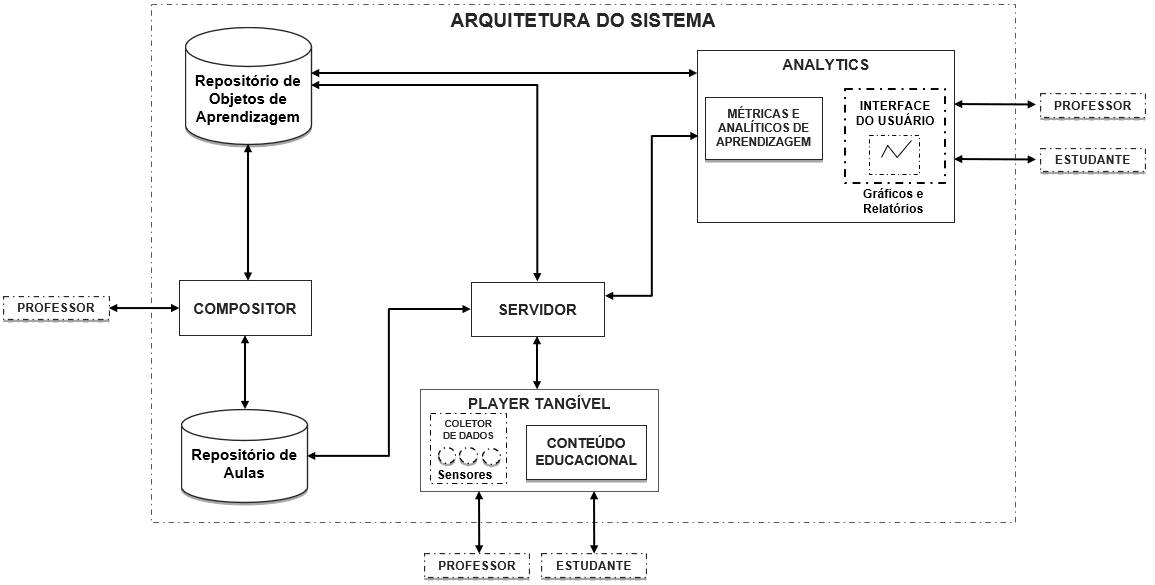
\includegraphics[width=1\linewidth]{chapters/proposedMethod/arquitetura_v4_1.png}
\caption{Arquitetura da Plataforma proposta}
\label{fig:arquitetura}
\end{figure}

De acordo com o Modelo apresentado na Figura~\ref{fig:arquitetura}, pode-se perceber que o professor interage e atua no ambiente educacional durante todo o processo, isto é, da composição e execução da aula até a visualização dos gráficos ou analíticos de aprendizagem gerados pelas interações dos estudantes com o conteúdo educacional, que acontecem apenas durante a aula e, sempre, mediadas pelo \textit{Player}.

Este capítulo é dividido em 4 seções. A primeira descreve o Compositor, os tipos de objetos de aprendizagem que são aceitos para a elaboração de uma aula, além da proposta de inclusão de objetos tangíveis de aprendizagem. A segunda seção apresenta o Servidor, que é responsável por agregar e armazenar os dados da interação dos estudantes com os dispositivos. Após isso, é apresentada a arquitetura do Player, que é responsável pela execução da aula, propriamente dita, e pela coleta dos dados de interação. Além de uma proposta de adição de objetos tangíveis de aprendizagem que permita interação entre suas partes física e digital. Por fim, a quarta seção aborda as métricas e analíticos de aprendizagem, ou seja, a parte do sistema responsável pelas análises dos dados e pela construção de gráficos para ajudar em tomadas de decisão que mais ajudem os estudantes nos processos de ensino-aprendizagem. %E, finalmente, a quinta seção apresenta um novo componente que serve de interface entre os módulos \textit{Servidor} e \textit{Analytics} e que aciona agentes que deem notificações ou façam recomendações adaptadas às percepções de contexto do estudante e às suas necessidades pedagógicas.
% , onde tais percepções e necessidades serão recebidas do componente analíticos.


\section{Compositor}\label{section:composer}
Essencialmente, este módulo atua como ferramenta e repositório de aulas e objetos de aprendizagem, de modo que é o responsável pela composição das aulas a partir de objetos de aprendizagem criados e/ou inseridos pelo professor, podendo também receber objetos provenientes de outros repositórios. É importante salientar que, em especial, o compositor permite a geração de objetos de aprendizagem como questionários avaliativos de múltipla-escolha e tangíveis. Outros objetos como slides, vídeos e imagens podem ser inseridos/trocados e utilizados na composição de uma aula, mas não podem ser editados pela ferramenta.

Para organização do sistema, foi criada uma hierarquia em que o maior nível é o da `Disciplina', dentro dele são cadastradas várias `Aulas', onde cada aula pode conter objetos de aprendizagem de diversos tipos. Além disso, estes objetos também estão ligados às disciplinas e a um professor que pode exercer o papel de autor desse objeto.

% %A Figura~\ref{fig:composerhierarquia} mostra a parte do Diagrama Entidade Relacionamento (Diagrama ER), que descreve a relação entre as entidades do banco de dados do Compositor. No extrato em questão, pode-se visualizar as entidades: \textit{user},\textit{Disciplina}, \textit{Aula} e \textit{Capitulo}.

% %\begin{figure}[h]
% %	\centering
% %	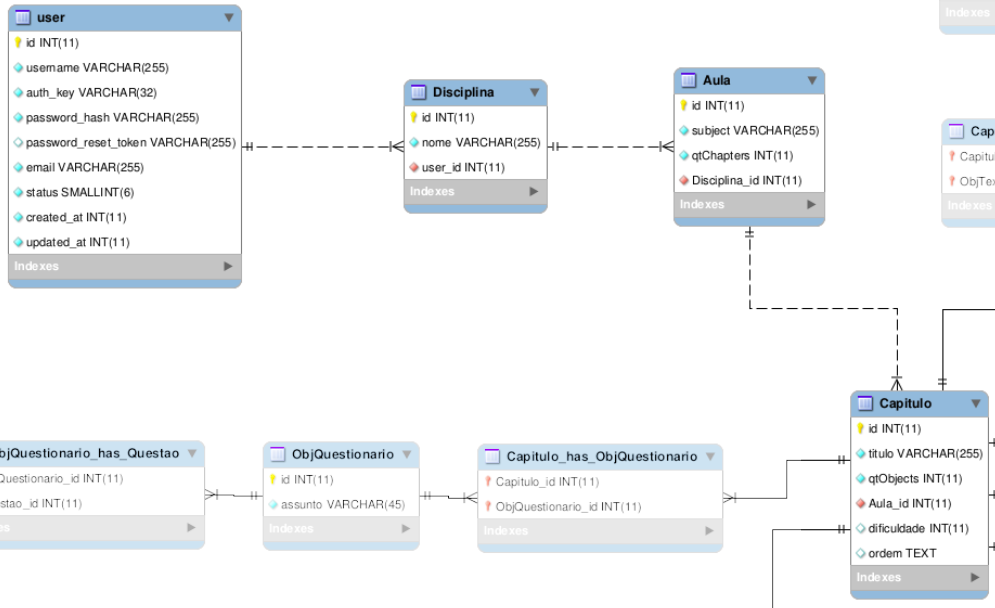
\includegraphics[width=1\linewidth]{imgs/ERComposer_hierarquiav2}
% %	\caption{Composer: entidades base}
% %	\label{fig:composerhierarquia}
% %\end{figure}

A Figura~\ref{fig:arquitetura_compositor} apresenta os principais componentes do Compositor, divididos em duas partes: (i) `Repositório de Aulas', onde é possível visualizar as entidades \textit{Disciplina}, \textit{Aula} e \textit{Objetos de Aprendizagem}, e (ii) `Repositório de Objetos de Aprendizagem', onde os objetos incluídos em uma aula podem ser acessados diretamente do banco de dados, especialmente, quando há reutilização de um objeto já armazenado. Além disso, há um destaque para a integração de objetos tangíveis de aprendizagem na plataforma.

\begin{figure}[htb]
	\centering
	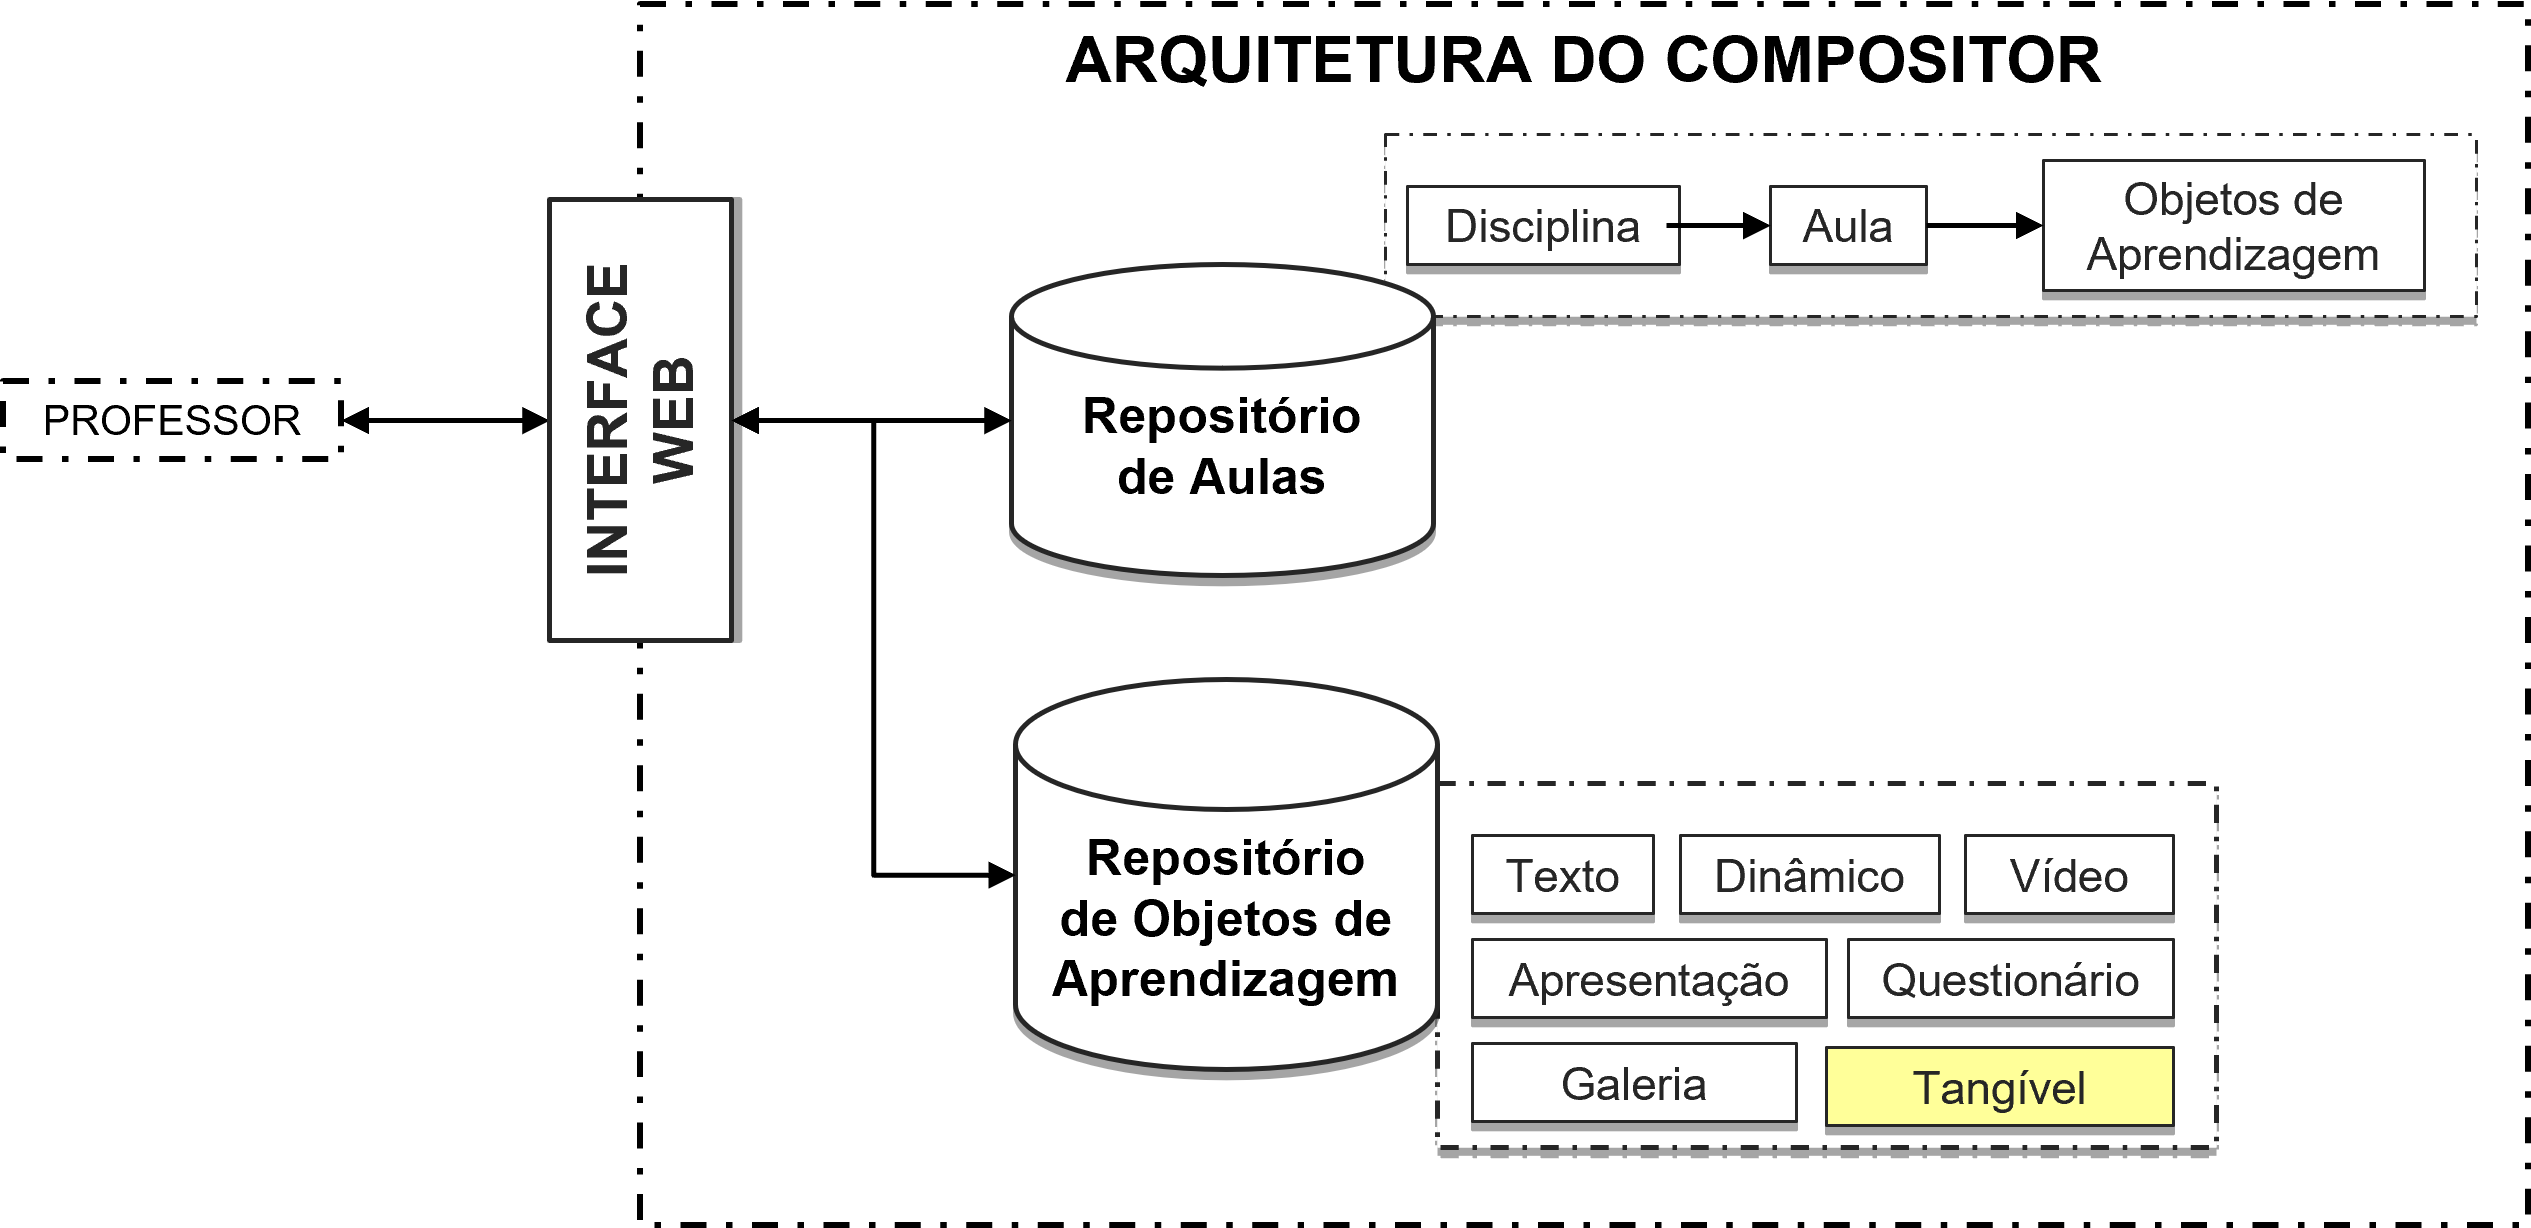
\includegraphics[width=0.9\linewidth]{chapters/proposedMethod/arquitetura_compositor.png}
	\caption{Compositor: arquitetura básica}
	\label{fig:arquitetura_compositor}
\end{figure}

Nesta abordagem, o banco de dados foi modelado para descrever os objetos de aprendizagem de tal modo que os seus metadados sejam compatíveis com os padrões IEEE-LOM e OBAA, tendo sido acrescentadas informações além do padrão relacionadas às métricas de aprendizagem e ao uso dos objetos tangíveis.

Com relação às métricas de aprendizagem (ver Seção~\ref{section:analytics}), considerando inicialmente objetos de aprendizagem do tipo questão de múltipla-escolha, foram acrescentadas informações relativas aos pesos das alternativas a serem escolhidas pelos alunos, além do tempo estimado pelo professor para que os alunos respondam a questão. Além disso, as informações relativas ao nível de dificuldade, previstas pelo IEEE-LOM e que são utilizadas na métrica de Nível de Compreensão, apresentada na Seção~\ref{section:analytics}, foram adaptadas com base no trabalho de~\cite{Biswas:2007}, onde são considerados apenas os níveis `Fácil`, `Normal' e `Difícil'.

% Nesta abordagem, cada Capítulo possui três níveis de dificuldade (`Fácil', `Normal' e `Difícil') previamente definidos pelo professor, quando da criação do mesmo. Além de ter relação com um ou mais capítulos, um objeto de aprendizagem possui um atributo `Conceito' que é o assunto específico tratado pelo objeto. Este atributo tem seu nível de dificuldade baseado nos mesmos três níveis dos Capítulos. Assim, tomando como exemplo, a disciplina de Física do currículo do Ensino Médio, tem-se o \textit{Capítulo} sobre `Oscilações, ondas, óptica e radiação' que tem nível de dificuldade `Difícil', onde é abordado o \textit{Conceito} de `Reflexão e Refração' que tem nível de dificuldade `Normal'.

% Essa classificação dos níveis do \textit{Capítulo} e do \textit{Conceito}, indicada pelo professor, será um elemento a ser levado em consideração nas métricas e análises de aprendizagem propostas neste trabalho. Entretanto, 
Para elaboração de uma aula completa, conceitualmente, o módulo Compositor aceita sete tipos de objetos de aprendizagem: (i) Galeria; (ii) Texto; (iii) Vídeo; (iv) Dinâmico; (v) Apresentação; (vi) Questionário; e, (vii) Tangível (Figura~\ref{fig:arquitetura_compositor}). Dos quais, os seis primeiros foram apresentados na dissertação de mestrado deste proponente~\citep{leitao:2017}.

% %\begin{figure}[h]
% %	\centering
% %	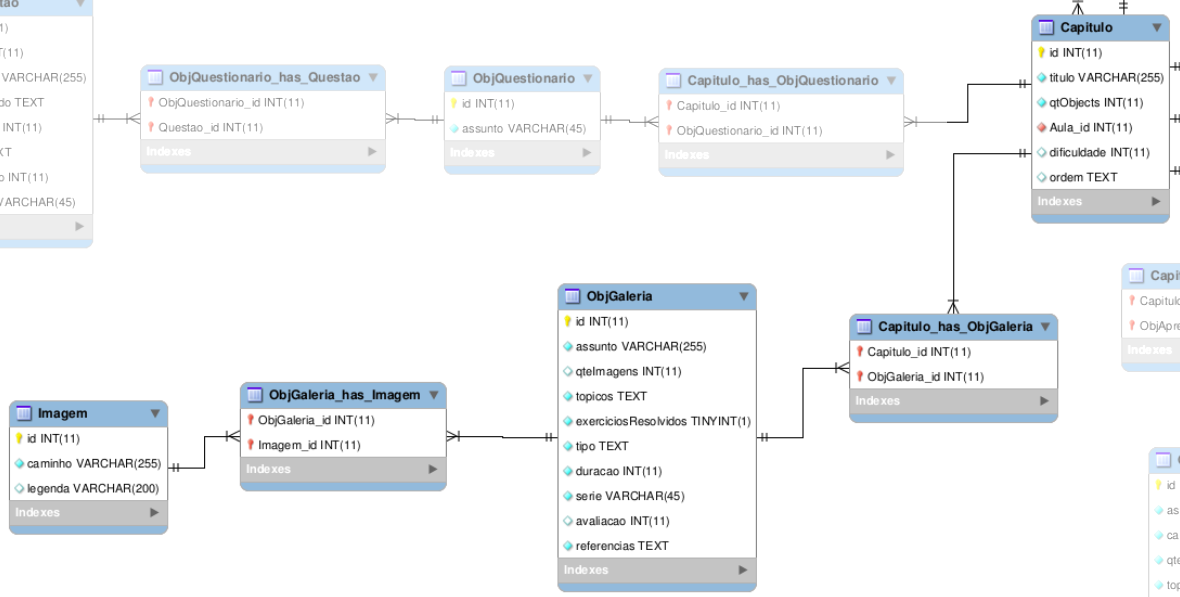
\includegraphics[width=1\linewidth]{imgs/ERComposer_galeriav2}
% %	\caption{Compositor: objetos `Galeria' e `Questionário'}
% %	\label{fig:composergaleria}
% %\end{figure}


Desse modo, o objeto `Galeria' corresponde a uma coleção de imagens, onde cada imagem é um objeto único no banco de dados e pode ser utilizada em diferentes galerias. O objeto `Texto' armazena conteúdos textuais da aula, podendo ser usado para descrição de atividades a serem feitas pela turma ou ainda para simples adição de conteúdos de texto sobre o tema a ser estudado.

O objeto `Vídeo' guarda informações relativas aos vídeos que serão exibidos durante uma aula, enquanto um objeto `Dinâmico' prevê a inserção de objetos com algum nível de interação, tais como \textit{applets} provenientes do Geogebra\footnote{Aplicativo de matemática que combina dinamicamente conceitos de geometria e álgebra em uma única interface do usuário.}. O objeto `Apresentação' corresponde aos \textit{slides} provenientes de ferramentas de escritório, sendo que o compositor converte todos os \textit{slides} em imagens, de modo a possibilitar a obtenção de informações mais precisas sobre a navegação do estudante neste tipo de objeto.

% %\begin{figure}[h]
% %	\centering
% %	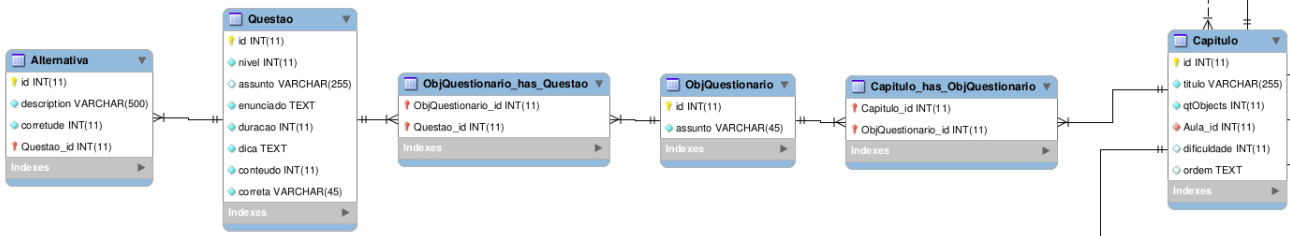
\includegraphics[width=1\linewidth]{imgs/ERComposer_questao}
% %	\caption{Compositor: 'Questionário'}
% %	\label{fig:composerquestionario}
% %\end{figure}

% \begin{figure}[ht]
% 	\centering
% 	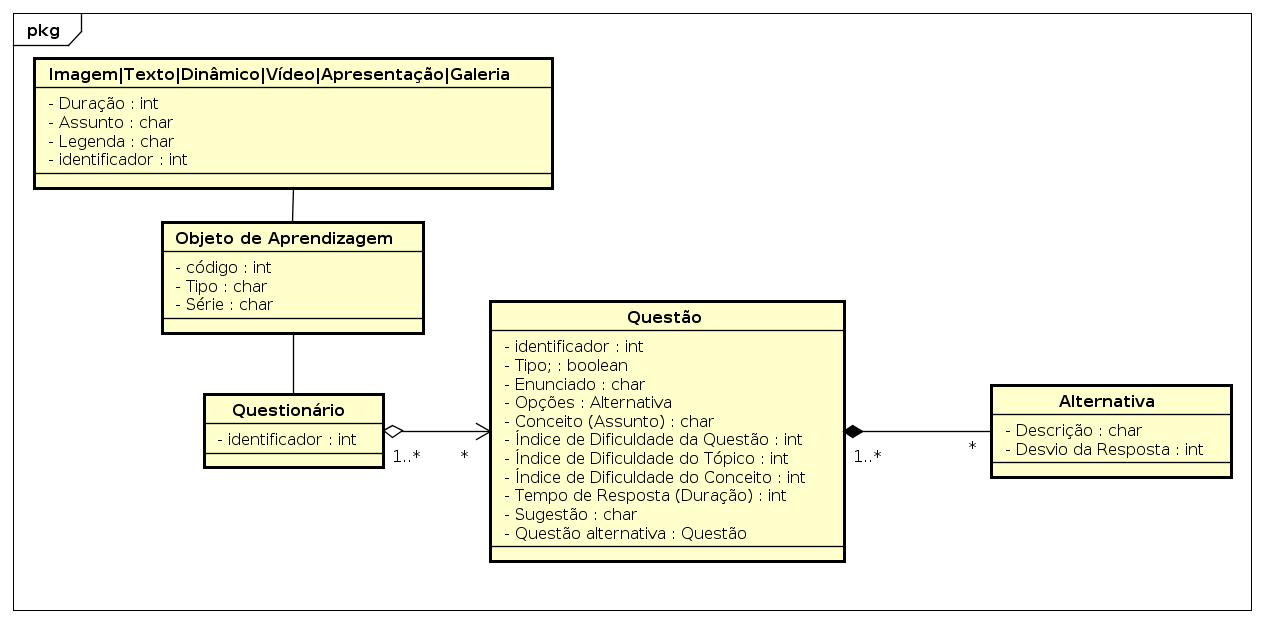
\includegraphics[width=1\linewidth]{imgs/Objetos_de_Aprendizagem}
% 	\caption{Compositor: Modelo dos Objetos de Aprendizagem}
% 	\label{fig:composerquestionario}
% \end{figure}

\textbf{OA Questionário}

O objeto de aprendizagem `Questionário' é uma coleção de questões para verificação do aprendizado do aluno de acordo com as métricas apresentadas na Seção~\ref{section:analytics}. Assim, como o objeto Galeria, cada questão cadastrada é um único objeto de aprendizagem que pode ser reutilizado em outros questionários.
% (Figura~\ref{fig:composerquestionario}). 

Ao criar uma questão, o autor do objeto deve inserir informações relativas ao `Índice de Dificuldade da Questão (IDQ)', `Índice de Dificuldade do Conteúdo (IDC)', `Tempo de Resposta do estudante', que é o tempo máximo esperado que o estudante responda a questão, e ao `Peso' de cada alternativa de resposta da Questão, que tem relação com a proximidade que uma alternativa está da resposta correta, isto é, quanto mais perto da resposta correta, maior o peso. 
%Essa proximidade é medida em cinco níveis, sendo melhor detalhada na Seção~\ref{sec:compreensao-questao}. 
A Figura~\ref{fig:compositor_questao} apresenta uma pré-visualização de um questionário no Compositor, onde é possível conferir esses elementos nos itens adicionados a um questionário.

\begin{figure}[htb]
	\centering
	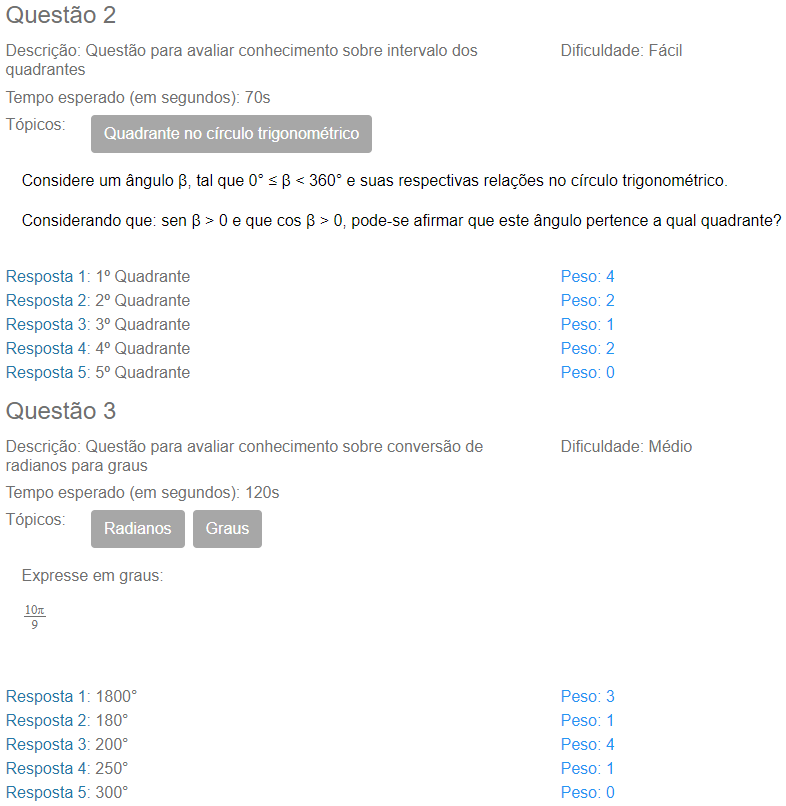
\includegraphics[width=0.9\linewidth]{chapters/proposedMethod/compositor_questoes.png}
	\caption{Compositor: Pré-visualização do Questionário}
	\label{fig:compositor_questao}
\end{figure}

% Além das informações já mencionadas, vale ressaltar que o questionário está inserido no contexto de uma proposta de ajuda sob demanda. Assim, a visualização e os recursos disponíveis, durante a resolução de uma questão, podem ser modificados de acordo com a percepção do sistema da dificuldade do estudante em dar uma resposta ao problema proposto.

% Como parte do mecanismo de modificação na aparência das questões, no momento da criação da questão, o professor precisará introduzir outros três elementos: (i) `Sugestão', que é uma frase ou parágrafo relacionado ao conteúdo que ajude a iluminar o problema; (ii) `Conceito', isto é, o assunto específico da questão, o que possibilitará uma consulta mais rápida e focada ao material didático fornecido; e (iii) `Questão Alternativa' que é uma questão sobre o mesmo assunto e com nível de dificuldade menor ou igual ao da questão principal. Assim, com a \textit{Sugestão} e o \textit{Conceito}, a questão alternativa também servirá como iluminação da resposta da questão principal.

% Na Figura~\ref{fig:composerquestao}, que representa uma questão com os atributos inseridos através do Compositor, pode-se observar tanto dados relacionados às métricas de aprendizagem quanto às opções de ajuda sob demanda.

% \begin{figure}[ht]
% 	\centering
% 	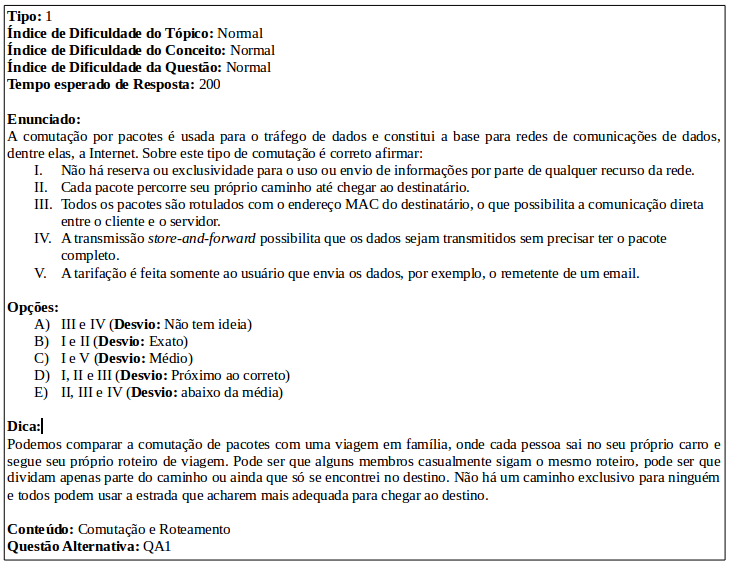
\includegraphics[width=1\linewidth]{imgs/exemplo_questao}
% 	\caption{Compositor: Exemplo de Atributos de uma Questão}
% 	\label{fig:composerquestao}
% \end{figure}

% %\begin{figure}[h]
% %	\centering
% %	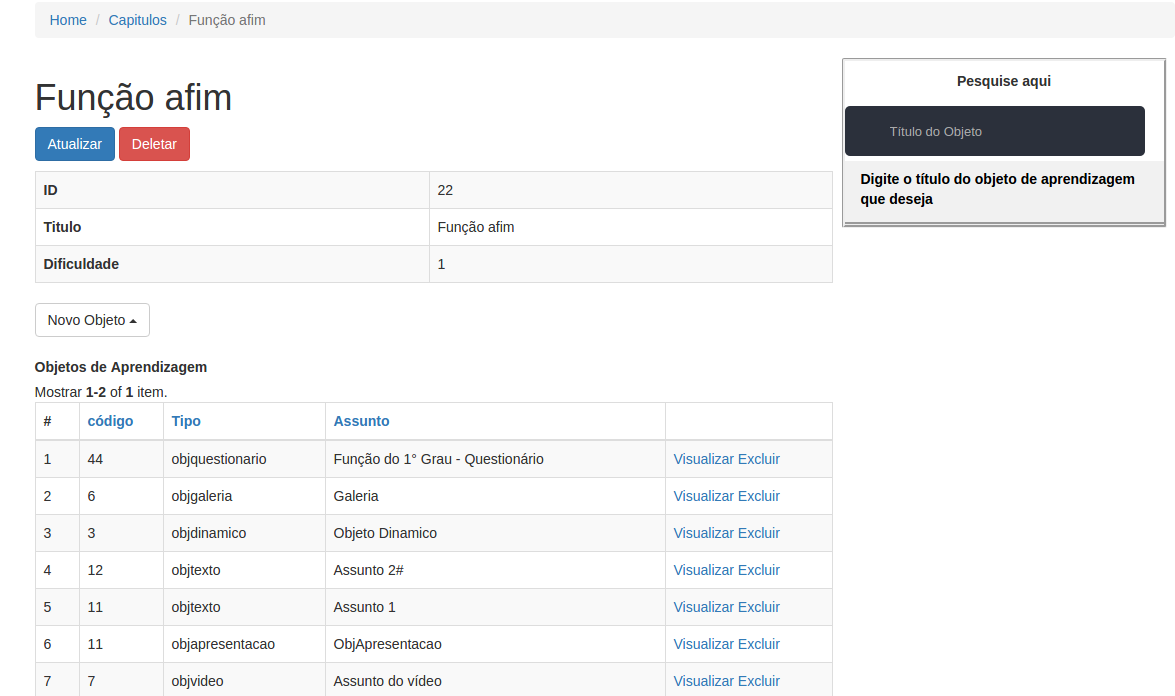
\includegraphics[width=1\linewidth]{imgs/composer}
% %	\caption{Exemplo de Tela do Composer}
% %	\label{fig:composer}
% %\end{figure}

% %A Figura~\ref{fig:composer} exibe uma tela com objetos de aprendizagem cadastrados no banco e associados a uma aula de Matemática. Tais objetos serão utilizados para compor o Player e serão utilizados durante a execução da aula presencial.

\textbf{OA Tangível}\label{section:OA_fisicovirtual}

Objetos Tangíveis de Aprendizagem (OTA) são manipulativos que contém, ao mesmo tempo, uma parte física e uma parte digital integradas entre si de modo que, ao ser criado no Compositor, cada OTA precisa ter componentes de ambas as partes devidamente instanciados e suas relações descritas.

Desse modo, será utilizado o conceito de objeto inteligente, apresentado na Seção~\ref{section:iot} e definido por \cite{serbanati:2011}, onde um objeto inteligente tem uma entidade digital e uma entidade física associadas através de um \textit{proxy} digital (vide p.~\pageref{fig:modeloiot}), de modo que o proxy digital atue como uma representação da entidade física no mundo digital. Além disso,~\cite{pires:2015} afirmam que um modelo de entidade virtual precisa ter um identificador unívoco e 
% um tipo (\textit{entityType}), 
atributos com informações sobre a entidade virtual e associação com os serviços que permitem o acesso aos recursos dos dispositivos por parte da entidade.

\begin{figure}[ht]
	\centering
	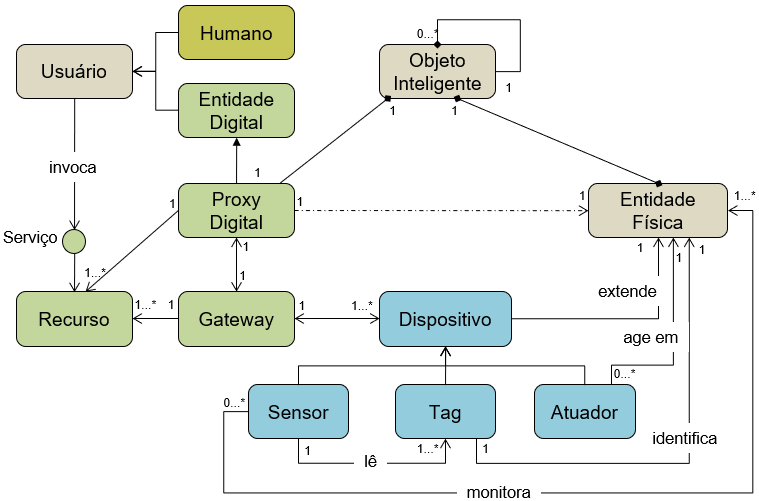
\includegraphics[width=0.8\linewidth]{chapters/proposedMethod/modelo_OTA.png}
	\caption{Modelo de Objeto Tangível de Aprendizagem proposto neste trabalho}
	\label{fig:modelo_ota}
\end{figure}

%Em vista disso, o modelo referencial de IoT apresentado na Figura~\ref{fig:modeloiot}, onde é definido um objeto inteligente com seus atributos e relações, foi adaptado para o modelo formal de objeto tangível de aprendizagem utilizado neste trabalho, de modo que um OTA contém quatro componentes principais: Dispositivos, \textit{Gateway}, Recursos e Serviços. Assim, Dispositivos são componentes de \textit{hardware} que funcionam como atuadores, TAGs e sensores e são utilizados na instrumentação do objeto, de modo que no contexto deste trabalho a descrição dos recursos é feita através de um código-fonte . Recursos são componentes digitais que fazem referência às propriedades físicas e digitais do objeto, de modo que as informações de ambas as partes possam ser recuperadas ou modificadas, assim, nesta proposta, a descrição dos Recursos corresponde a definição das variáveis de entrada e saída físicas e virtuais.
Em vista disso, o modelo referencial de IoT apresentado por \cite{serbanati:2011} que define um objeto inteligente, seus atributos e relações foi adaptado conforme apresentado na Figura~\ref{fig:modelo_ota}, e servirá de modelo para o objeto tangível de aprendizagem utilizado neste trabalho, de modo que um objeto tangível de aprendizagem proposto nestes termos contém quatro componentes principais: Dispositivos, \textit{Gateway}, Recursos e Serviços. 

Assim, Dispositivos são os componentes de \textit{hardware} que funcionam como atuadores, TAGs e sensores e são utilizados na instrumentação do objeto de aprendizagem. O Gateway é um componente que garante o acesso aos Dispositivos e deve ser executado em um microcontrolador com capacidade de transmissão e recepção de pacotes de mensagens, de modo que a comunicação entre as entidades física e a virtual do objeto seja estabelecida através de um protocolo de troca de mensagens.

Recursos são componentes digitais que fazem referência às propriedades físicas e digitais do objeto, de modo que as informações de ambas as partes possam ser recuperadas ou modificadas. Assim, nesta proposta, a descrição dos Recursos corresponde a definição das variáveis de entrada e saída físicas e virtuais.

\begin{figure}[htb]
	\centering
	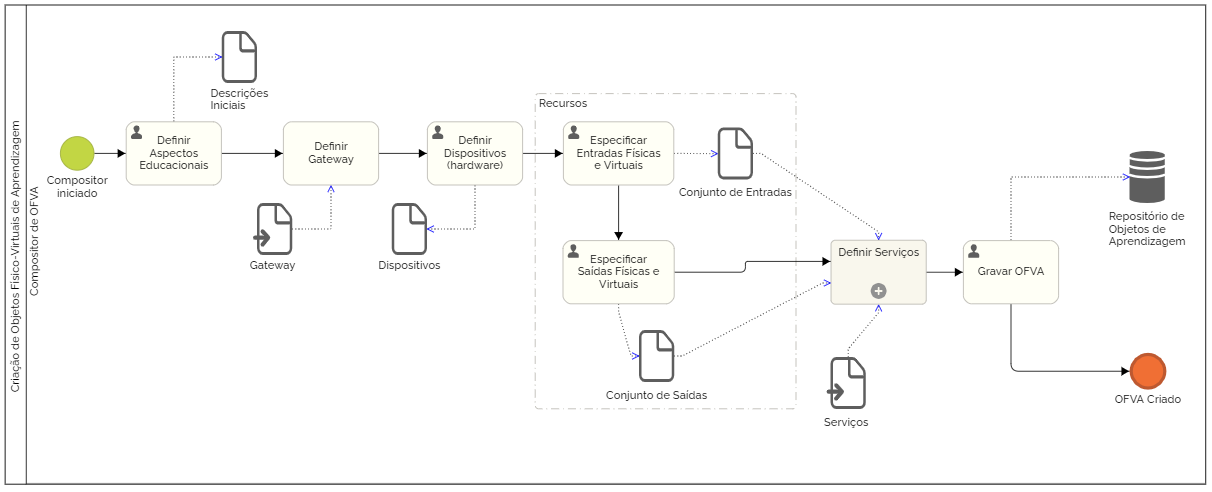
\includegraphics[width=1\linewidth]{chapters/proposedMethod/bpmn_ofva.png}
	\caption{Modelo BPMN para Criação de OTAs vinculados a uma plataforma educacional}
	\label{fig:bpmn_ofva}
\end{figure}

Além disso, é preciso que o compositor de objetos de aprendizagem seja capaz de integrar um manipulativo físico, instrumentado com sensores diversos, a um conjunto de páginas web que implementam um manipulativo virtual, com entradas e saídas equivalentes ao físico, de modo que o produto do processo seja um objeto com ambos os manipulativos físico e virtual integrados como um único objeto físico/digital de aprendizagem. Assim, o componente Serviços descreve e implementa as ações que estarão disponíveis ao usuário no Player (ver Seção~\ref{section:player}) e que garantem ao estudante o acesso aos Recursos do OTA, de modo que são especificados tanto os componentes necessários a execução da entidade digital associada ao objeto físico (páginas web, componentes javascript) quanto quais entradas e saídas físicas e digitais serão utilizadas em cada caso de teste com suas respectivas regras de avaliação da aprendizagem e \textit{feedback}, conforme o necessário (Figura~\ref{fig:bpmn_ofva_casos}).

\begin{figure}[htb]
	\centering
	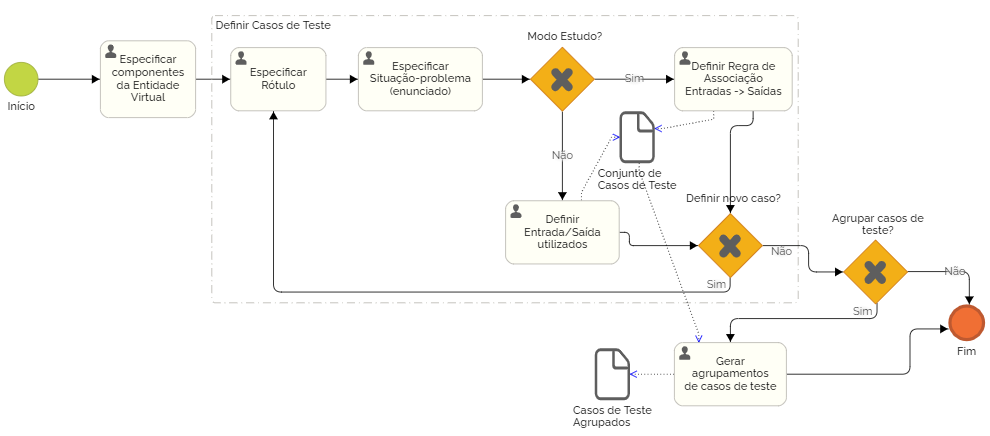
\includegraphics[width=0.9\linewidth]{chapters/proposedMethod/bpmn_servicos.png}
	\caption{Subprocesso `Definir Serviços'}
	\label{fig:bpmn_ofva_casos}
\end{figure}

É importante salientar que, no contexto deste trabalho, um caso de teste equivale uma situação-problema que pode ser instrumentada com parâmetros (regras) que permitam ao Player auxiliar o estudante no caminho de construção do conhecimento, de modo que ele possa corrigir as suas respostas até que descubra a resposta correta ao utilizar o objeto tangível no \textbf{modo estudo}. Além disso, para que o objeto tangível seja utilizado para o acompanhamento/avaliação da aprendizagem, um caso de teste também precisa estar associado aos parâmetros das diversas métricas propostas neste trabalho (Seção~\ref{section:analytics}).

%Além disso, para que o fluxo desse processo aconteça conforme o necessário, é preciso que o compositor de objetos de aprendizagem seja capaz de integrar um manipulativo físico instrumentado com sensores diversos a um conjunto de páginas web que implementam um manipulativo virtual com entradas e saídas equivalentes ao físico, de modo que o produto do processo seja um objeto com ambos os manipulativos físico e virtual integrados como um único objeto físico-virtual de aprendizagem.

A fim de formalizar esta proposta, diagramas de processos BPMN (\textit{Business Process Model and Notation}) foram definidos de modo a orientar os passos para composição de um OTA. Assim, as Figuras \ref{fig:bpmn_ofva} e \ref{fig:bpmn_ofva_casos} apresentam o modelo, onde o autor dos objetos de aprendizagem precisa definir: (i) aspectos educacionais do OTA; (ii) gateway; (iii) dispositivos (hardware); (iv) recursos (entradas e saídas físicas e virtuais) e (v) serviços (componentes digitais e casos de teste). A Tabela~\ref{tabela:OFV} detalha os atributos necessários para a construção de um objeto tangível de aprendizagem conforme o modelo proposto.

% Entretanto, para a formalização da instanciação dos elementos dos OFV e facilitar a comunicação entre os componentes da plataforma deverá ser definida uma linguagem de marcação que consiga descrever os atributos e dados coletados de cada objeto físico-virtual de aprendizagem. Dentre as opções de linguagens estão a OWL e a EEML que são muito utilizadas para essa finalidade, estando presentes em quase todas os \textit{middleware} IoT apresentados por~\cite{pires:2015}. Em vista das limitações inerentes a estas linguagens, deverá ser feita uma extensão dos seus elementos para que possibilitem uma descrição mais adequada dos dados coletados provenientes dos diversos sensores ou atuadores.


\begin{table}[htb]
\caption{Atributos de um Objeto Tangível de Aprendizagem}
\centering

\begin{tabularx}{\textwidth}{|c|X|}
\hline
\textbf{Atributo} & \textbf{Descrição} \\ \hline
\textbf{ID} & Identificador unívoco do OTA \\ \hline
\textbf{Título} & Nome do OTA \\ \hline
\textbf{Descrição Geral} & Descrição textual acerca do conteúdo do OTA \\ \hline
\textbf{Descrição Educacional} & Descrição acerca de como o OTA deve ser usado \\ \hline
\textbf{Tópicos} & Conceitos abordados pelo OTA \\ \hline
\textbf{Modo} & -\textbf{Estudo}: modo com \textit{feedbacks} em tempo de interação do aluno com dicas sobre o tópico estudado e a posteriori das métricas de aprendizagem;

	-\textbf{Avaliação}: modo apenas com \textit{feedback} a posteriori das métricas de aprendizagem\\ \hline
\textbf{Gateway} & Código-fonte a ser executado em um microcontrolador\\ \hline
\textbf{Dispositivos} & Sensores, tags ou atuadores que compõem o OTA\\ \hline
\textbf{Recursos} & Conjuntos de Entradas e Saídas Físicas e Digitais com rótulos, tipos de dado e valores\\ \hline
\textbf{Serviços} &  -\textbf{Componentes Digitais} da Entidade Virtual (páginas web, javascripts,...); 

-\textbf{Casos de Teste}: Situações-problema a serem resolvidas pelos estudantes com fins de acompanhamento/verificação da aprendizagem. É necessário indicar os parâmetros das métricas de avaliação propostas neste trabalho (níveis de dificuldade, pesos, tempo...). \\ \hline
\end{tabularx}
\label{tabela:OFV}
\end{table}

Adicionalmente, o Compositor de OTA utiliza uma linguagem de programação em blocos baseada na biblioteca Blockly~\citep{Blockly:2022} para definição das Entradas e Saídas e das regras dos Casos de Teste (Figura~\ref{fig:blockly_exemplo}). Tais elementos serão utilizados pela plataforma para comunicação e respostas do servidor às ações dos estudantes na parte virtual, inclusive com relação às respostas esperadas para as situações-problema definidas pelo autor do objeto de aprendizagem, uma vez que Blockly permite a tradução da lógica dos blocos para outras linguagens de programação como JavaScript (Figura~\ref{fig:blockly_exemplo}), PHP e Python.

\begin{figure}[ht]
	\centering
	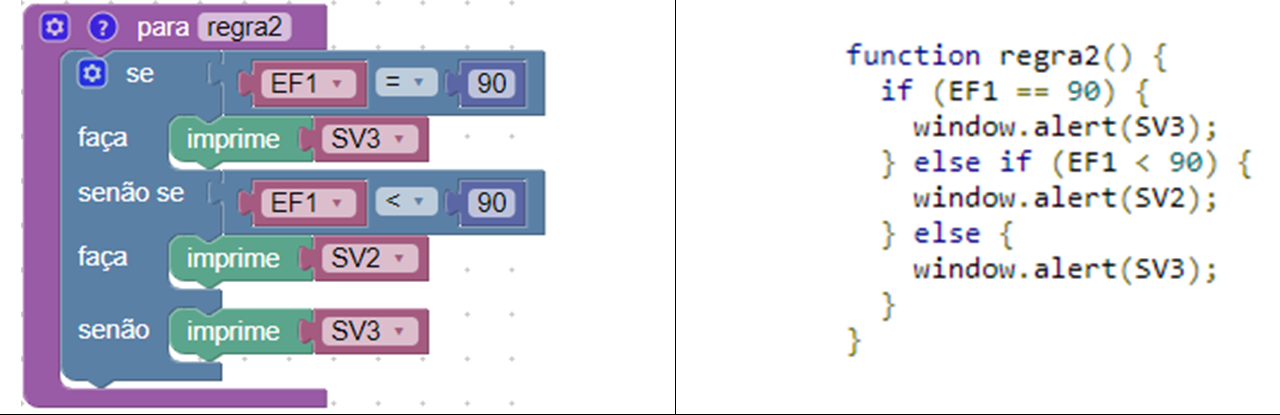
\includegraphics[width=1\linewidth]{chapters/proposedMethod/Blockly.png}
	\caption{Exemplo de definição de regra para caso de teste e sua tradução para linguagem JavaScript}
	\label{fig:blockly_exemplo}
\end{figure}


Além disso, é importante ressaltar que, ao desafio de modelar e padronizar os objetos tangíveis de aprendizagem, acrescentam-se: (i) a demanda por uma descrição adequada dos seus metadados de modo a facilitar não apenas a criação de repositórios, mas, a recomendação e o reuso desses tipos de objetos; e, (ii) a necessidade de estabelecer critérios de avaliação e verificação do aprendizado de maneira automática.

\textbf{Padrão de Metadados}

Com relação a descrição dos metadados, após estudar alguns dos padrões existentes como Dublin Core, IEEE-LOM e OBAA, optou-se pelo último, que é derivado do padrão IEEE-LOM. Essa opção foi feita pelo fato do OBAA ser um padrão brasileiro presente implementado em importantes repositórios de objetos de aprendizagem nacionais, além de oferecer suporte a mídias de diferentes plataformas, dentre elas, TV Digital, Web e Móveis, ter descritores educacionais com uma base epistemológica interacionista e descritores de acessibilidade~\citep{vicari:2009}.

Assim, inicialmente, foi escolhido o perfil compatível ideal com o OBAA denominado ``PM-OBAA-FULL''. Entretanto, para melhor descrição dos objetos de aprendizagem que estamos usando, alguns dos descritores fora do perfil ideal padrão foram utilizados. A tabela do Apêndice~\ref{Chap:AppendixA} apresenta os descritores atualmente utilizados. 

%\textbf{ATUALIZAR TEXTO A SEGUIR: Além disso, nos próximos passos, a pesquisa será aprofundada com vistas a propor uma extensão do padrão OBAA que descreva adequadamente objetos físico-virtuais de aprendizagem.}

\section{Servidor}\label{section:service}
É o módulo que cria uma sala de aula virtual, gerencia as trocas de mensagens entre os dispositivos dos estudantes e do professor, além de consolidar os dados para análise de acordo com as métricas de aprendizagem propostas. Com a adição dos objetos tangíveis de aprendizagem, o Servidor também tratará os dados provenientes da interação dos estudantes com ambas as partes física e digital do objeto, além de disponibilizar acesso aos recursos virtuais do OTA.

% além de realizar modificações na apresentação das questões, segundo uma abordagem de percepção da dificuldade dos estudantes.

\begin{figure}[htbp]
	\centering
	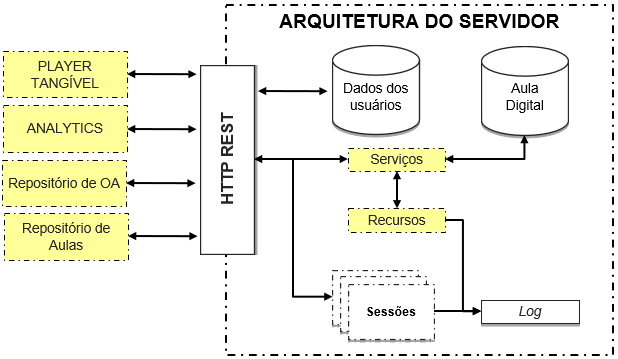
\includegraphics[width=0.8\linewidth]{chapters/proposedMethod/arquitetura_servidor.png}
	\caption{Arquitetura do Servidor}
	\label{fig:servidor}
\end{figure}

Inicialmente, o professor disponibiliza através do Servidor a aula a ser ministrada juntamente com as informações da turma que terá aula (por exemplo: nome, matrícula, senha,...). Esse carregamento é necessário pois, por decisão de projeto, a plataforma foi implementada de modo a levar em consideração que o acesso a internet em escolas periféricas brasileiras pode ser restrito ou inexistente e, no caso amazônico, essas escolas também podem estar situadas em municípios interioranos ou comunidades ribeirinhas. Dessa forma, o protótipo de servidor que gerencia a aula contendo o objeto tangível implementado neste trabalho provê a condução da aula sem uma conexão com a internet.

Após o carregamento da aula e das turmas relacionadas, uma sessão é criada para cada aluno que se conecta ao Servidor e, além disso, o conteúdo da aula é disponibilizado via \textit{streaming} para cada dispositivo conectado de acordo com as requisições HTTP Rest executadas. Desse modo, o Servidor terá uma tripla finalidade: (i) gerenciar as conexões dos alunos com a finalidade de coletar dados e armazenar \textit{logs} de interação dos estudantes com o material didático; (ii) prover acesso às possíveis notificações e recomendações pedagógicas; e, (iii) prover acesso aos recursos dos objetos de aprendizagem.
% e, de acordo com as dificuldades apresentadas pelos alunos na hora de responder um questionário avaliativo, apresentar recursos adicionais de ajuda. 

A Figura~\ref{fig:servidor} destaca em amarelo as modificações feitas na estrutura do servidor em relação ao proposto originalmente por~\cite{leitao:2017}, em especial os acréscimos necessários para que o mesmo trabalhe com objetos tangíveis de aprendizagem. Desse modo, podemos observar um novo componente correspondente aos  ``Recursos'', que é responsável por referenciar as entradas e saídas físicas e digitais do objeto com o objetivo de armazenar essas interações no log. O segundo componente adicionado corresponde aos ``Serviços'' disponibilizados pelo Player e que estão armazenados no banco de dados, tais serviços correspondem ao conteúdo dos objetos (ie: páginas web, códigos em javascript que proveem o \textit{feedback} do modo estudo).

Por fim, pode-se notar que a comunicação com os módulos Analytics, o novo Player Tangível e os repositórios de objetos de aprendizagem e de aulas acontece via HTTP Rest.

\section{Player Tangível}\label{section:player}
% %É um conjunto de páginas web contendo todo o material didático de uma aula a ser ministrada (Figura~\ref{fig:aulaplayer}). Tais páginas são executadas em um navegador de internet, onde acontece a interação do estudante com o material didático.

% %\begin{figure}[h]
% %\centering
% %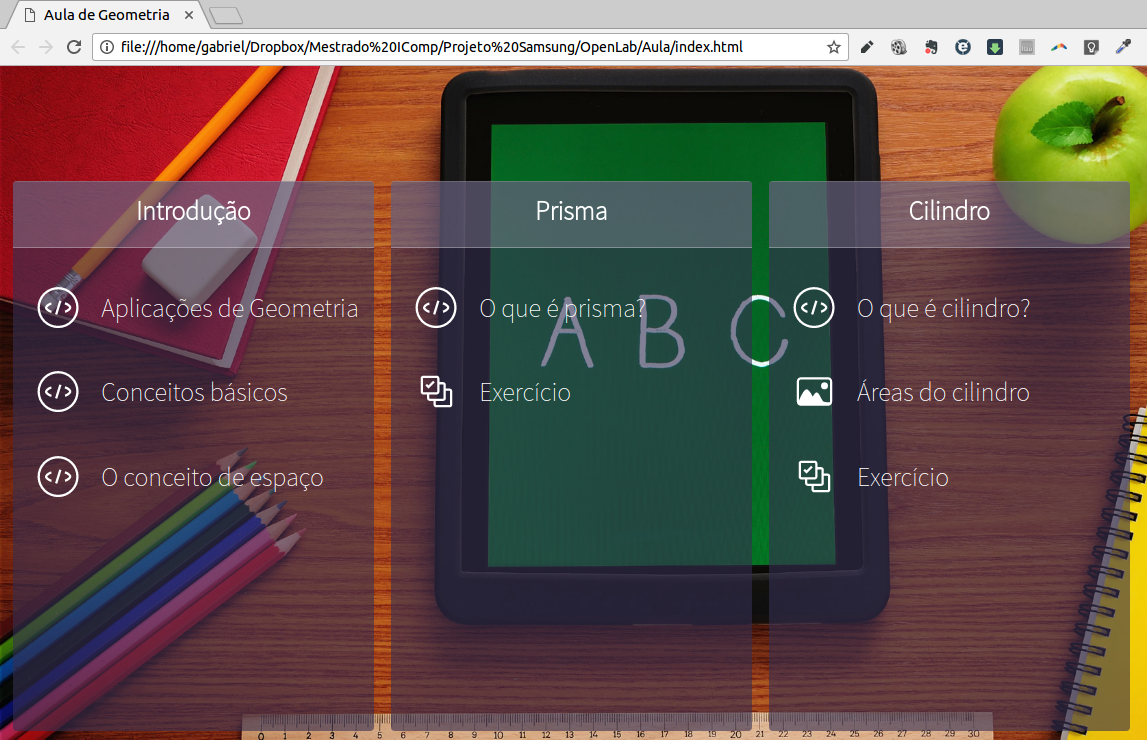
\includegraphics[width=0.75\linewidth]{imgs/player_aulageometria}
% %\caption{Exemplo de aula sendo executada no Player}
% %\label{fig:aulaplayer}
% %\end{figure}

O Player apresentado por~\cite{leitao:2017}, é definido como um conjunto de páginas web contendo todo o material didático de uma aula a ser ministrada, de modo que tais páginas são executadas em um navegador de internet, através do qual acontece a interação do estudante com o conteúdo educacional. O Player Tangível expande esse conceito de modo que o novo \textit{player} conta com uma interface física (manipulativo físico instrumentado com sensores) cuja interação do aluno reflete na sua respectiva interface digital.

Assim, enquanto o Player tradicional possui duas partes principais (Figura~\ref{fig:arquiteturaplayer}): (i) Aula Digital; (ii) Coletor de Dados; onde, a `Aula Digital' é o material didático baseado em web e o `Coletor de Dados' é um rastreador que coleta os cliques dos alunos. O conceito de Player Tangível acrescenta uma terceira parte relacionada a `entidade física' que é integrada a sua respectiva contraparte `entidade digital' através do \textit{Gateway}. 

Assim, o que para \cite{leitao:2017} corresponde a aula digital provendo os diversos objetos de aprendizagem tradicionais (questionários, slides, vídeos,...), neste trabalho, o mesmo componente provê também a entidade digital do objeto tangível, correspondendo assim ao \textit{proxy digital} do objeto físico/digital. Ademais, na entidade física, pode-se notar a presença dos componentes `Dispositivos', `Gateway' e `Recursos' definidos no modelo proposto de um objeto tangível (Figura~\ref{fig:modelo_ota}) conforme a proposta deste trabalho. O componente `Serviços' serve de ponte para ambas as interfaces física e digital de modo que as entradas físicas e digitais correspondentes e o conteúdo educacional sejam acessados pelos estudantes.

%de `controle de objeto' atrelada aos `atributos' deste objeto (entradas físicas e virtuais e regras dos casos de teste) de modo a proporcionar a comunicação em tempo real entre as partes física e virtual, de modo que toda manipulação física do aluno é refletida automaticamente na sua parte virtual.

% É essa interação do Coletor com o Servidor que viabilizará os três níveis de ajuda sob demanda apresentados nas Seções~\ref{section:composer} e \ref{section:service}.

\begin{figure}[htb]
	\centering
	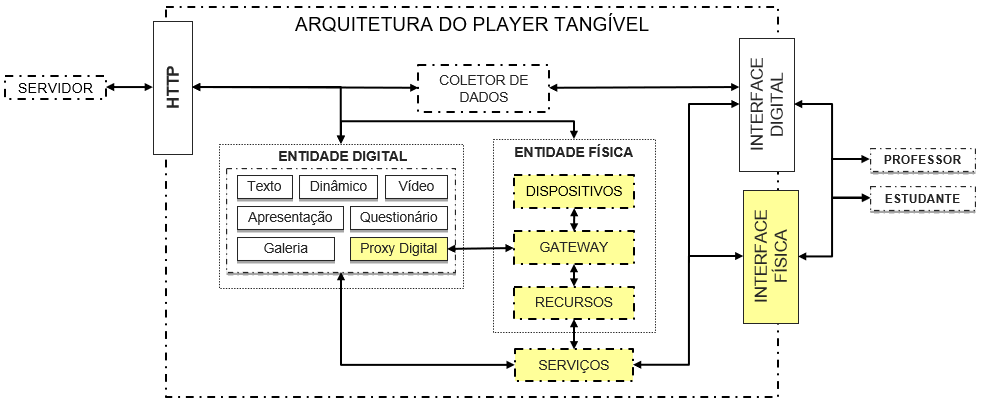
\includegraphics[width=1\linewidth]{chapters/proposedMethod/arquitetura_player.png}
	\caption{Arquitetura do Player Tangível}
	\label{fig:arquiteturaplayer}
\end{figure}

Assim, a proposta de Player Tangível apresentada neste trabalho conta com duas interfaces de comunicação com o usuário (professores ou estudantes), uma baseada em web e outra baseada em manipulativo físico. A interface digital permite a entrega do conteúdo educacional digital em praticamente qualquer dispositivo e plataforma sem necessidade de instalação de \textit{softwares} adicionais. Essa característica possibilita grande portabilidade dessa parte do sistema e, por conseguinte, baixo custo de implantação, visto que cada aluno pode, por exemplo, usar seu próprio dispositivo móvel durante a aula. Essa abordagem visa não apenas inserir definitivamente as novas tecnologias em sala de aula, mas, tirar proveito dos recursos que os estudantes trazem consigo, além de tentar aumentar o nível de engajamento do estudante em uma aula.

Por fim, é importante notar que a interface física está atrelada ao manipulativo físico utilizado, o qual deve possuir um conjunto de dados que o descrevam, incluindo informações acerca dos sensores utilizados, dos formatos de dados e das ações executadas como resposta às interações dos estudantes (conforme especificado nas regras dos casos de teste). Assim como os outros objetos de aprendizagem, os OTA também tem seus dados de interação coletados pelo sistema com a finalidade de viabilizar uma análise inteligente da aprendizagem que permita extrair conhecimentos sobre o comportamento e o desempenho dos estudantes para, no futuro, propor recursos ou estratégias educacionais que colaborem efetivamente na melhoria da aprendizagem.

%Dentre os dados a serem descritos, além dos necessários ao funcionamento do OTA que devem ser descritos em alguma linguagem que permita a associação com sensores tais como OWL ou EEML, é importante ressaltar a necessidade de se estender algum padrão de metadados de modo a descrever adequadamente estes objetos.

\subsection{Processo de conexão entre as entidades física e digital}\label{sub:JSON}

Em termos de ferramenta, propomos a utilização do protocolo \textit{Websocket} de modo a tornar a comunicação em tempo real mais eficiente, onde o \textit{Gateway} apresentado no Modelo de Referência (Figura~\ref{fig:modelo_ota}) como elemento de integração entre as entidades física e digital foi implementado, nesta proposta de Tese, como um servidor \textit{Websocket} (ver Subseção~\ref{subsec:tools_player}). 

Além disso, como parte da formalização desta proposta, para o processo de troca de mensagens com o Gateway, foi escolhido o formato \textit{JSON} de modo a garantir que maior compatibilidade entre as partes física e digital, de modo que a Tabela~\ref{tabela:JSON} apresenta uma descrição inicial dos principais campos utilizados no formato definido, que serão detalhados no decorrer desta seção.

% Please add the following required packages to your document preamble:
% \usepackage[table,xcdraw]{xcolor}
% If you use beamer only pass "xcolor=table" option, i.e. \documentclass[xcolor=table]{beamer}
\begin{table}[htb]
	\caption{Campos para troca de mensagens entre as entidades do Player Tangível}
	\centering
	\begin{tabular}{|c|c|c|c|}
		\hline
		\rowcolor[HTML]{C0C0C0} 
		\textbf{Campo} & \textbf{Tipo} & \textbf{Descrição} & \textbf{Observação} \\ \hline
		type & string & Tipo da mensagem & Obrigatório \\ \hline
		action & string & Ação a ser realizada & Obrigatório \\ \hline
		data & object & Informação específica de cada mensagem & Opcional \\ \hline
		error & object & Detalhes do erro & Opcional \\ \hline
	\end{tabular}
	\label{tabela:JSON}
\end{table}

A Listagem~\ref{JSON_exemplo} apresenta um exemplo inicial de modelo para o formato JSON a ser utilizado nas mensagens trocadas, note-se que alguns dos campos possuem subcampos que especificam mais informações.

\begin{listing}[htb]
	\begin{minted}[frame=lines,framesep=2mm,fontsize=\footnotesize,linenos]{json}
		{
			"type": "connection",
			"action": "connect",
			"data": {
				"connected": false,
			},
			"error": {
				"code": 1,
				"message": "Já existe um usuário conectado"
			}
		}
	\end{minted}
	\caption{Exemplo de mensagem JSON}
	\label{JSON_exemplo}
\end{listing}

\textbf{Conexão via \textit{Websocket} e preparação para pareamento}

O passo inicial para o pareamento entre as entidades física e virtual é o estabelecimento de uma conexão via \textit{websocket}, por onde todas as mensagens no formato JSON serão trocadas. Assim, a Figura~\ref{fig:diagrama-websockets} apresenta o diagrama de sequência que ilustra esse processo, onde pode-se notar que, após o estudante inserir o número identificador único da entidade física (URI) na parte virtual do Player Tangível, as mensagens seguintes estabelecem primeiro um canal \textit{websocket} e, em seguida, é feita uma primeira troca de mensagens para verificação da possibilidade de pareamento entre as entidades.

\begin{figure}[htb]
	\centering
	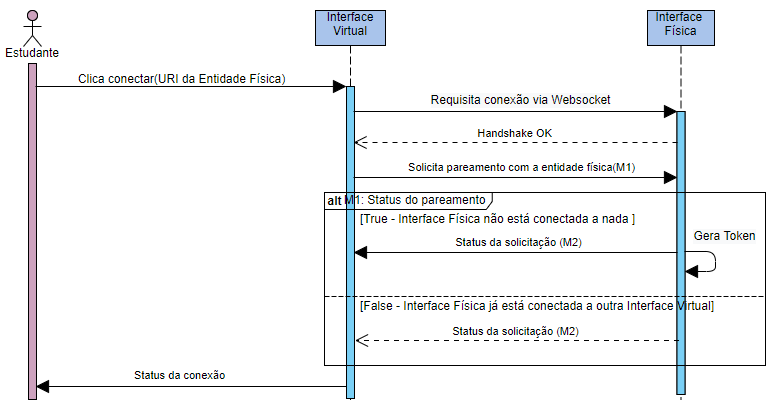
\includegraphics[width=0.9\linewidth]{chapters/proposedMethod/msg_websocket.png}
	\caption{Diagrama de Sequência - Conexão Websocket}
	\label{fig:diagrama-websockets}
\end{figure}

%A Tabela~\ref{tab:websocket} detalha a mensagens que devem ser trocadas durante esta etapa prévia ao pareamento. 
É importante notar que após a confirmação do \textit{handshake}, a interface virtual envia automaticamente a mensagem $M1$ de solicitação de pareamento (Tabela~\ref{tab:websocket}), obtendo como resposta a mensagem $M2$, que pode ser tanto de confirmação quanto de recusa da solicitação. 

\begin{table}[htb]
	\centering
	\caption{Mensagem de solicitação de pareamento}
	\begin{tabular}{|c|ccc|}
		\hline
		\rowcolor[HTML]{C0C0C0} 
		\textbf{Mensagem} & \multicolumn{3}{c|}{\cellcolor[HTML]{C0C0C0}\textbf{Descrição}} \\ \hline
		M1 & \multicolumn{3}{c|}{Solicitar pareamento} \\ \hline
		\rowcolor[HTML]{C0C0C0} 
		\textbf{Campo} & \multicolumn{1}{c|}{\cellcolor[HTML]{C0C0C0}\textbf{Tipo}} & \multicolumn{1}{c|}{\cellcolor[HTML]{C0C0C0}\textbf{Valor}} & \textbf{Observação} \\ \hline
		\textit{type} & \multicolumn{1}{c|}{\textit{string}} & \multicolumn{1}{c|}{\textit{connection}} & \multicolumn{1}{l|}{} \\ \hline
		\textit{action} & \multicolumn{1}{c|}{\textit{string}} & \multicolumn{1}{c|}{\textit{connect}} & \multicolumn{1}{l|}{} \\ \hline
	\end{tabular}
	\label{tab:websocket}
\end{table}

Uma mensagem de confirmação permite o prosseguimento do processo de pareamento, de modo que a interface física gera um número de \textit{token} que deve ser informado em até 30 segundos através da interface virtual.

\begin{table}[htb]
	\centering
	\caption{Mensagens de solicitação e de status da solicitação de pareamento}
\begin{tabular}{|c|ccc|}
	\hline
	\rowcolor[HTML]{C0C0C0} 
	\textbf{Mensagem} & \multicolumn{3}{c|}{\cellcolor[HTML]{C0C0C0}\textbf{Descrição}} \\ \hline
	M2 & \multicolumn{3}{c|}{Status da solicitação} \\ \hline
	\rowcolor[HTML]{C0C0C0} 
	\textbf{Campo} & \multicolumn{1}{c|}{\cellcolor[HTML]{C0C0C0}\textbf{Tipo}} & \multicolumn{1}{c|}{\cellcolor[HTML]{C0C0C0}\textbf{Valor}} & \textbf{Observação} \\ \hline
	\textit{type} & \multicolumn{1}{c|}{\textit{string}} & \multicolumn{1}{c|}{\textit{connection}} &  \\ \hline
	\textit{action} & \multicolumn{1}{c|}{\textit{string}} & \multicolumn{1}{c|}{\textit{connect}} &  \\ \hline
	\textit{data.connected} & \multicolumn{1}{c|}{\textit{boolean}} & \multicolumn{1}{c|}{\textit{true | false}} & \begin{tabular}[c]{@{}c@{}}Solicitação recebida com\\ sucesso | Erro no \\pareamento\end{tabular} \\ \hline
	\textit{data.expires\_in} & \multicolumn{1}{c|}{\textit{integer}} & \multicolumn{1}{c|}{30} & \begin{tabular}[c]{@{}c@{}}Tempo de espera para \\ recebimento do Token\end{tabular} \\ \hline
	\textit{error.code} & \multicolumn{1}{c|}{\textit{integer}} & \multicolumn{1}{c|}{1} &  \\ \hline
	\textit{error.message} & \multicolumn{1}{c|}{string} & \multicolumn{1}{c|}{Já existe um usuário conectado} & \begin{tabular}[c]{@{}c@{}}Só é permitida uma conexão \\ por dispositivo físico\end{tabular} \\ \hline
\end{tabular}
	\label{tab:websocketstatus}
\end{table}

Já uma mensagem de recusa de pareamento por parte da entidade física encerra o processo com o código de erro `1' e a mensagem `Já existe um usuário conectado', uma vez que uma entidade física só pode se conectar a uma única entidade virtual.

\textbf{Mensagens relativas ao pareamento}

Quando a interface virtual recebe um \textit{status} de confirmação da solicitação ($M2$ é verdadeiro), então, o usuário tem trinta segundos para inserir na interface virtual e enviar o \textit{token} aleatório que aparece na tela da interface física. Assim, a validação do \textit{token} é solicitada através da mensagem $M3$, que é enviada pela interface virtual para a parte física (vide Figura~\ref{fig:diagrama-token} e Tabela~\ref{tab:tokenM3}).

\begin{figure}[htb]
	\centering
	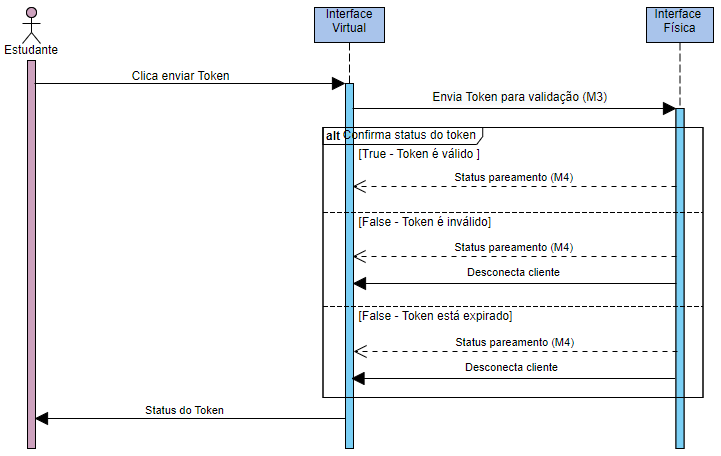
\includegraphics[width=0.9\linewidth]{chapters/proposedMethod/msg_token.png}
	\caption{Diagrama de Sequência para Pareamento}
	\label{fig:diagrama-token}
\end{figure}

A mensagem $M4$ ocorre quando a entidade física retorna o status do pareamento para a entidade virtual. Essa mensagem pode ser de confirmação (\textit{true}) ou de recusa de pareamento (\textit{false}), conforme ilustrado na Figura~\ref{fig:diagrama-token}. Em caso de confirmação, o status do token para o usuário é dado pela atualização da interface virtual de modo que a entidade virtual se torna visível e passa a exibir a mesma aparência e posição dos elementos da entidade física.

\begin{table}[htb]
	\centering
	\caption{Solicitação de validação do \textit{token}}
	\begin{tabular}{|c|ccc|}
		\hline
		\rowcolor[HTML]{C0C0C0} 
		\textbf{Mensagem} & \multicolumn{3}{c|}{\cellcolor[HTML]{C0C0C0}\textbf{Descrição}} \\ \hline
		M3 & \multicolumn{3}{c|}{Envia Token para validação} \\ \hline
		\rowcolor[HTML]{C0C0C0} 
		\textbf{Campo} & \multicolumn{1}{c|}{\cellcolor[HTML]{C0C0C0}\textbf{Tipo}} & \multicolumn{1}{c|}{\cellcolor[HTML]{C0C0C0}\textbf{Valor}} & \textbf{Observação} \\ \hline
		\textit{type} & \multicolumn{1}{c|}{\textit{string}} & \multicolumn{1}{c|}{\textit{connection}} &  \\ \hline
		\textit{action} & \multicolumn{1}{c|}{\textit{string}} & \multicolumn{1}{c|}{\textit{token}} &  \\ \hline
		data.token & \multicolumn{1}{c|}{string} & \multicolumn{1}{c|}{Token informado pelo usuário} &  \\ \hline
	\end{tabular}
	\label{tab:tokenM3}	
\end{table}

Caso ocorra recusa no pareamento por parte da entidade física, a mensagem $M4$ retorna um dos erros especificados na Tabela~\ref{tab:tokenM4}. De modo que, o erro `2' corresponde a mensagem de que o token informado é inválido por não ser igual ao token mostrado na tela da entidade física e, o erro `3' é relativo ao fato de que o tempo de validade do token expirou. Para o segundo caso, é gerado um novo token com um novo tempo de validade.

\begin{table}[htb]
	\centering
	\caption{Mensagem para validação do \textit{token}}
	\begin{tabular}{|c|ccc|}
		\hline
		\rowcolor[HTML]{C0C0C0} 
		\textbf{Mensagem} & \multicolumn{1}{c|}{\cellcolor[HTML]{C0C0C0}\textbf{Descrição}} & \multicolumn{1}{c|}{\cellcolor[HTML]{C0C0C0}\textbf{}} & \textbf{} \\ \hline
		M4 & \multicolumn{3}{c|}{Status do pareamento} \\ \hline
		\rowcolor[HTML]{C0C0C0} 
		\textbf{Campo} & \multicolumn{1}{c|}{\cellcolor[HTML]{C0C0C0}\textbf{Tipo}} & \multicolumn{1}{c|}{\cellcolor[HTML]{C0C0C0}\textbf{Valor}} & \textbf{Observação} \\ \hline
		\textit{type} & \multicolumn{1}{c|}{\textit{string}} & \multicolumn{1}{c|}{\textit{connection}} & \multicolumn{1}{l|}{} \\ \hline
		\textit{action} & \multicolumn{1}{c|}{\textit{string}} & \multicolumn{1}{c|}{\textit{token}} & \multicolumn{1}{l|}{} \\ \hline
		\textit{data.is\_valid\_token} & \multicolumn{1}{c|}{\textit{boolean}} & \multicolumn{1}{c|}{\textit{true | false}} & \multicolumn{1}{l|}{\begin{tabular}[c]{@{}l@{}}True: Token é válido. \\ False: Token informado é \\ inválido ou o tempo de \\ validação expirou (erro é\\ detalhado)\end{tabular}} \\ \hline
		\textit{error.code} & \multicolumn{1}{c|}{\textit{integer}} & \multicolumn{1}{c|}{2 | 3} & \multicolumn{1}{l|}{\begin{tabular}[c]{@{}l@{}}2: Token inválido\\ 3: Token expirado\end{tabular}} \\ \hline
		\textit{error.message} & \multicolumn{1}{c|}{string} & \multicolumn{1}{c|}{\begin{tabular}[c]{@{}c@{}}2:Token inválido\\ 3: Token expirado\end{tabular}} & \multicolumn{1}{l|}{\begin{tabular}[c]{@{}l@{}}2: O token enviado pelo \\ virtual não coincide com \\ o gerado pelo físico.\\ 3: O tempo para validação\\ do token expirou. É \\ necessário gerar um novo.\end{tabular}} \\ \hline
	\end{tabular}
	\label{tab:tokenM4}	
\end{table}


\textbf{Envio de Dados}

Com o estabelecimento da conexão entre as entidades física e virtual, qualquer manipulação captada pelos sensores presentes no artefato físico deve refletir na sua respectiva contraparte virtual, de modo que, a partir deste momento, todas as mensagens enviadas da parte física para a virtual são relativas a atualização das posições do manipulativo físico e correspondem às entradas físicas definidas no projeto do objeto tangível, de modo que a mensagem $M5$ é encarregada de transmitir estas informações utilizando os campos constantes na Tabela~\ref{tab:dadosEF}.

\begin{table}[htb]
	\centering
	\caption{Mensagem para envio de dados da entrada física}
	\begin{tabular}{|c|ccc|}
		\hline
		\rowcolor[HTML]{C0C0C0} 
		\textbf{Mensagem} & \multicolumn{3}{c|}{\cellcolor[HTML]{C0C0C0}\textbf{Descrição}} \\ \hline
		M5 & \multicolumn{3}{c|}{Envia dados} \\ \hline
		\rowcolor[HTML]{C0C0C0} 
		\textbf{Campo} & \multicolumn{1}{c|}{\cellcolor[HTML]{C0C0C0}\textbf{Tipo}} & \multicolumn{1}{c|}{\cellcolor[HTML]{C0C0C0}\textbf{Valor}} & \textbf{Observação} \\ \hline
		\textit{type} & \multicolumn{1}{c|}{\textit{string}} & \multicolumn{1}{c|}{\textit{physical}} &  \\ \hline
		\textit{action} & \multicolumn{1}{c|}{\textit{string}} & \multicolumn{1}{c|}{\textit{message}} &  \\ \hline
		data.input & \multicolumn{1}{c|}{string} & \multicolumn{1}{c|}{Nome da entrada física} &  \\ \hline
		\textit{data.value} & \multicolumn{1}{c|}{\textit{integer | float}} & \multicolumn{1}{c|}{Dado enviado} & \multicolumn{1}{l|}{\begin{tabular}[c]{@{}l@{}}Este campo pode assumir \\ diversos tipos de acordo \\ com a necessidade\end{tabular}} \\ \hline
	\end{tabular}
	\label{tab:dadosEF}	
\end{table}

Do mesmo modo, eventuais manipulações na entidade virtual também devem ser refletidas na sua contraparte física (através de atuadores), se essas manipulações virtuais estiverem previstas na concepção do objeto tangível. A Tabela~\ref{tab:dadosSF} apresenta os campos que devem constar na mensagem $M6$, responsável por essa troca de informações.

\begin{table}[htb]
	\centering
	\caption{Mensagem para envio de dados para a saída física}
	\begin{tabular}{|c|ccc|}
		\hline
		\rowcolor[HTML]{C0C0C0} 
		\textbf{Mensagem} & \multicolumn{3}{c|}{\cellcolor[HTML]{C0C0C0}\textbf{Descrição}} \\ \hline
		M6 & \multicolumn{3}{c|}{Envia dados} \\ \hline
		\rowcolor[HTML]{C0C0C0} 
		\textbf{Campo} & \multicolumn{1}{c|}{\cellcolor[HTML]{C0C0C0}\textbf{Tipo}} & \multicolumn{1}{c|}{\cellcolor[HTML]{C0C0C0}\textbf{Valor}} & \textbf{Observação} \\ \hline
		\textit{type} & \multicolumn{1}{c|}{\textit{string}} & \multicolumn{1}{c|}{\textit{physical}} &  \\ \hline
		\textit{action} & \multicolumn{1}{c|}{\textit{string}} & \multicolumn{1}{c|}{\textit{message}} &  \\ \hline
		data.output & \multicolumn{1}{c|}{string} & \multicolumn{1}{c|}{Nome da saída física} &  \\ \hline
		\textit{data.value} & \multicolumn{1}{c|}{\textit{integer | float}} & \multicolumn{1}{c|}{Dado enviado} & \multicolumn{1}{l|}{\begin{tabular}[c]{@{}l@{}}Este campo pode assumir \\ diversos tipos de acordo \\ com a necessidade\end{tabular}} \\ \hline
	\end{tabular}
	\label{tab:dadosSF}	
\end{table}

Eventualmente, pode ser requisitado que o estudante não apenas manipule a parte física, mas, além disso, envia uma mensagem indicando que cessou a manipulação. Nesses casos, a mensagem $M6$ é enviada pela entidade física conforme o especificado na Tabela~\ref{tab:dadosConfirmacao}.

\begin{table}[htb]
	\centering
	\caption{Mensagem para envio de resposta}
	\begin{tabular}{|c|ccc|}
		\hline
		\rowcolor[HTML]{C0C0C0} 
		\textbf{Mensagem} & \multicolumn{3}{c|}{\cellcolor[HTML]{C0C0C0}\textbf{Descrição}} \\ \hline
		M7 & \multicolumn{3}{c|}{Envia resposta} \\ \hline
		\rowcolor[HTML]{C0C0C0} 
		\textbf{Campo} & \multicolumn{1}{c|}{\cellcolor[HTML]{C0C0C0}\textbf{Tipo}} & \multicolumn{1}{c|}{\cellcolor[HTML]{C0C0C0}\textbf{Valor}} & \textbf{Observação} \\ \hline
		\textit{type} & \multicolumn{1}{c|}{\textit{string}} & \multicolumn{1}{c|}{\textit{physical}} &  \\ \hline
		\textit{action} & \multicolumn{1}{c|}{\textit{string}} & \multicolumn{1}{c|}{\textit{message}} &  \\ \hline
		data.input & \multicolumn{1}{c|}{string} & \multicolumn{1}{c|}{Nome da entrada física} &  \\ \hline
		\textit{data.value} & \multicolumn{1}{c|}{\textit{integer | float}} & \multicolumn{1}{c|}{Dado enviado} & \multicolumn{1}{l|}{\begin{tabular}[c]{@{}l@{}}Este campo pode assumir \\ diversos tipos de acordo \\ com a necessidade\end{tabular}} \\ \hline
		data.confirm & \multicolumn{1}{c|}{boolean} & \multicolumn{1}{c|}{True} & \multicolumn{1}{l|}{\begin{tabular}[c]{@{}l@{}}Confirma que é uma \\ mensagem de resposta e \\ não de atualização de \\ posição\end{tabular}} \\ \hline
	\end{tabular}
	\label{tab:dadosConfirmacao}	
\end{table}

Por fim, o diagrama de sequência da Figura~\ref{fig:diagrama-dados} ilustra os três tipos de mensagens que podem ser enviadas durante este processo de envio de dados. É importante notar que o estudante é representado em ambas as pontas do diagrama, ora interagindo com a interface física, ora com a virtual.

\begin{figure}[htb]
	\centering
	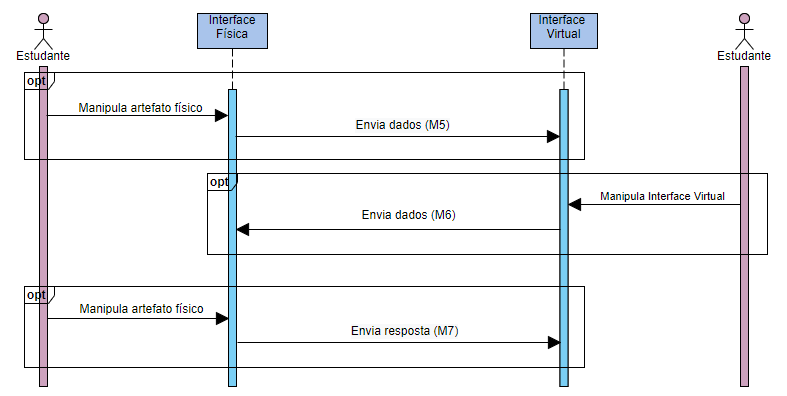
\includegraphics[width=0.9\linewidth]{chapters/proposedMethod/msg_dadosv2.png}
	\caption{Diagrama de Sequência para envio de dados}
	\label{fig:diagrama-dados}
\end{figure}


\textbf{Mensagens de reconexão e desconexão}

Durante uma aula, o estudante pode transitar entre diferentes objetos de aprendizagem, de modo que é necessário prever que, em caso de saída da interface virtual para acessar outro objeto (i.e: uma apresentação ou um questionário) e um eventual retorno a mesma interface, embora a conexão via websocket seja mantida, o navegador web precisa garantir que ambas as entidades (física e virtual) estão corretamente pareadas. 

Assim, a interface física pode requisitar uma reconexão através da mensagem $M8$, conforme os campos apresentados na Tabela~\ref{tab:reconexao}, onde nota-se que o conteúdo do campo \textit{data.token} desta mensagem contém o último \textit{token} inserido pelo usuário. Esse procedimento acontece para que a entidade física consiga reconhecer a virtual sem a necessidade de o usuário inserir um novo token a cada vez que precise utilizar outro objeto de aprendizagem.

\begin{table}[htb]
	\centering
	\caption{Mensagem para solicitação de reconexão}
	\begin{tabular}{|c|ccc|}
		\hline
		\rowcolor[HTML]{C0C0C0} 
		\textbf{Mensagem} & \multicolumn{3}{c|}{\cellcolor[HTML]{C0C0C0}\textbf{Descrição}} \\ \hline
		M8 & \multicolumn{3}{c|}{Solicita reconexão} \\ \hline
		\rowcolor[HTML]{C0C0C0} 
		\textbf{Campo} & \multicolumn{1}{c|}{\cellcolor[HTML]{C0C0C0}\textbf{Tipo}} & \multicolumn{1}{c|}{\cellcolor[HTML]{C0C0C0}\textbf{Valor}} & \textbf{Observação} \\ \hline
		\textit{type} & \multicolumn{1}{c|}{\textit{string}} & \multicolumn{1}{c|}{\textit{connection}} &  \\ \hline
		\textit{action} & \multicolumn{1}{c|}{\textit{string}} & \multicolumn{1}{c|}{\textit{reconnect}} &  \\ \hline
		data.token & \multicolumn{1}{c|}{string} & \multicolumn{1}{c|}{Último token guardado} & \multicolumn{1}{l|}{\begin{tabular}[c]{@{}l@{}}Reenvia o último token \\ utilizado\end{tabular}} \\ \hline
	\end{tabular}
	\label{tab:reconexao}	
\end{table}

A Figura~\ref{fig:diagrama-reconexao} indica que a solicitação de reconexão feita pela entidade virtual deve ser respondida pela entidade física através de uma mensagem $M4$, de modo que o comportamento da interface virtual seja o mesmo de quando do estabelecimento de uma nova conexão, isto é, o status de confirmação do token faz com que a entidade virtual apareça para o usuário e seja automaticamente atualizada com os dados de posição provenientes da entidade física.

\begin{figure}[htb]
	\centering
	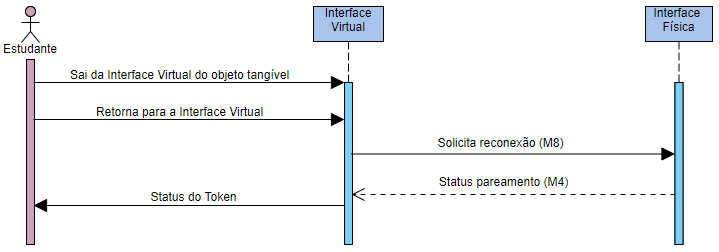
\includegraphics[width=0.9\linewidth]{chapters/proposedMethod/msg_reconexao.png}
	\caption{Diagrama de Sequência para reconexão}
	\label{fig:diagrama-reconexao}
\end{figure}

%o envio de dados entre as entidades deve cessar a fim de evitar tráfego de dados desnecessário na rede.

Por fim, a última mensagem definida é a de desconexão (Tabela~\ref{tab:desconexao}) e deve ocorrer quando um usuário solicita a saída (\textit{logout}) do ambiente tangível de aprendizagem, encerrando sua participação na aula.

\begin{table}[htb]
	\centering
	\caption{Mensagem para solicitação de desconexão}
	\begin{tabular}{|c|ccc|}
		\hline
		\rowcolor[HTML]{C0C0C0} 
		\textbf{Mensagem} & \multicolumn{3}{c|}{\cellcolor[HTML]{C0C0C0}\textbf{Descrição}} \\ \hline
		M9 & \multicolumn{3}{c|}{Solicita desconexão} \\ \hline
		\rowcolor[HTML]{C0C0C0} 
		\textbf{Campo} & \multicolumn{1}{c|}{\cellcolor[HTML]{C0C0C0}\textbf{Tipo}} & \multicolumn{1}{c|}{\cellcolor[HTML]{C0C0C0}\textbf{Valor}} & \textbf{Observação} \\ \hline
		\textit{type} & \multicolumn{1}{c|}{\textit{string}} & \multicolumn{1}{c|}{\textit{connection}} &  \\ \hline
		\textit{action} & \multicolumn{1}{c|}{\textit{string}} & \multicolumn{1}{c|}{\textit{disconnect}} &  \\ \hline
	\end{tabular}
	\label{tab:desconexao}	
\end{table}


\section{Analíticos}\label{section:analytics}

Neste trabalho, \textit{Analíticos} é a parte do sistema que utiliza os dados de interação dos estudantes com o ambiente de aprendizagem para calcular métricas que sirvam 
%de novas ``features''
tanto para avaliar e acompanhar a aprendizagem quanto para gerar análises de dificuldades e necessidades dos estudantes.
Desse modo, este trabalho propõe a adoção de oito métricas para medir tanto a interação do estudante com o material didático quanto o seu desempenho em atividades educacionais. Além disso, algumas dessas métricas são baseadas no trabalho de~\cite{Biswas:2007} e uma delas é exatamente o modo tradicional de calcular a pontuação de um estudante, isto é, baseando-se apenas nos seus acertos e erros.

Estas métricas podem ser divididas em duas partes: (i) cinco métricas independentes (Nota Tradicional, Nota Ponderada, Dúvida da Questão, Grau de Assertividade, Tempo de Resposta); e (ii) três métricas baseadas na composição de outras métricas (Prioridade, Nível de Compreensão da Questão, Nível de Compreensão).
%Estas métricas podem ser divididas em duas partes: (i) sete métricas independentes (Nota Tradicional, Nota Ponderada, Desvio da Resposta, Dúvida da Questão, Grau de Assertividade, Tempo de Resposta, Nível de Desordem); e (ii) quatro métricas baseadas na composição de outras métricas (Desvio do Conjunto, Prioridade, Nível de Compreensão da Questão, Nível de Compreensão)

\subsection{Métricas Independentes}
O conjunto das métricas de avaliação da aprendizagem apresentadas nesta subseção corresponde aquelas que podem ser consideradas isoladas, no sentido de que não dependem de um cálculo anterior de outras métricas. 

\subsubsection{Nota Tradicional}\label{sec:nota-tradicional}

É a métrica mais comum para calcular a pontuação de um aluno, sendo uma medida de precisão entre a quantidade de respostas corretas ($rc$) e o número total de questões ($n$). Dessa métrica, podemos definir a taxa de erro como o complemento da \textbf{Nota Tradicional (NT)} por $e=1-NT$. A pontuação e o erro tradicionais são normalizados no intervalo $[0,1]$, mas, costuma-se apresentar a pontuação no intervalo $[0,10]$, conforme a Equação~\ref{eq:NT}.

\begin{equation}\label{eq:NT}
NT=10\cdot \frac{rc}{n}
\end{equation}

Como exemplo, podemos considerar um questionário de seis questões, onde um estudante que acerta todas as seis questões, pela Equação~\ref{eq:NT}, obtém uma pontuação igual a ``10'' e um estudante que responde corretamente apenas cinco questões, obtém ``8,33''.

Neste trabalho, argumentamos que a Nota Tradicional não é suficiente para avaliar corretamente o desempenho do aluno, de modo que, nas Seções~\ref{sec:level-understanding} e~\ref{sec:learningvectors} expusemos algumas métricas encontradas na literatura para avaliar o grau de conhecimento do aluno e produzir uma pontuação.

Assim, nas próximas subseções, proporemos oito novas métricas para avaliação de estudantes em ambientes de aprendizagem apoiados por tecnologia e que podem ser aproveitadas para uso em diversos tipos de objetos de aprendizagem, dentre eles, os objetos físico-virtuais propostos neste trabalho.

\subsubsection{Nota Ponderada}\label{sec:nota-ponderada}

\textbf{Nota Ponderada (NP)} é outra pontuação que pode ser apresentada no intervalo $[0,10]$, mas, que é baseada no peso ($p_i$) de cada resposta selecionada e na pontuação ponderada máxima ($pmp$). A Equação~\ref{eq:NP} mostra a fórmula $NP$, onde o valor do peso das respostas de cada questão ($p_i$) é um número inteiro de 0 a 4, onde 0 significa resposta totalmente errada, 4 significa resposta totalmente correta e os outros são respostas intermediárias (veja Tabela~\ref{tab:Pesos}).
A pontuação máxima ponderada ($pmp$) é simplesmente a quantidade total de perguntas no questionário ($n$) multiplicada por 4.

\begin{table}[htbp]
\caption{Pesos das respostas - p}
\centering
\begin{tabular}{|c|c|c|c|c|c|}
\hline
\textbf{Peso} & \textbf{Não tem ideia} & \textbf{Abaixo do Meio} & \textbf{Meio} & \textbf{Quase correto} & \textbf{Correto} \\ \hline
\textbf{Valor} & 0 & 1 & 2 & 3 & 4 \\ \hline
\end{tabular}
\label{tab:Pesos}
\end{table}

\begin{equation}
\label{eq:NP}
NP = 10 \cdot \frac{\sum_{i=1}^n p_i}{ppm}
\end{equation}

onde\\
\indent $p_i$ é proveniente da Tabela~\ref{tab:Pesos};\\
$ppm = $n$ \cdot 4$; e\\
$n$ é o total de questões no questionário.

A Tabela~\ref{tab:notas-estudantes} será usada como exemplo para explicar algumas métricas propostas neste trabalho. Ela mostra as notas de um aluno de acordo com os pesos das opções de resposta selecionadas em duas disciplinas. Além disso, as questões na cor verde correspondem aos verdadeiros positivos (acertos) e as questões em vermelho correspondem às respondidas incorretamente.

\begin{table}[ht]
\caption{Notas do Estudante}
\centering
\begin{tabular}{|c|c|c|c|c|c|c|c|}
\hline
\multicolumn{8}{|c|}{\cellcolor[HTML]{000000}{\color[HTML]{FFFFFF} \textbf{DISCIPLINA ``A''}}} \\ \hline
\textbf{$n$ = 6; pmp=24} & \cellcolor[HTML]{009901}Q1 & \cellcolor[HTML]{FE0000}\textbf{Q2} & \cellcolor[HTML]{009901}\textbf{Q3} & \cellcolor[HTML]{FE0000}\textbf{Q4} & \cellcolor[HTML]{009901}\textbf{Q5} & \cellcolor[HTML]{009901}\textbf{Q6} & \textbf{Total} \\ \hline
\textbf{p$_j$} & \textbf{4} & \textbf{3} & \textbf{4} & \textbf{2} & \textbf{4} & \textbf{4} & \textbf{21}  \\ \hline
\multicolumn{8}{|c|}{\cellcolor[HTML]{000000}{\color[HTML]{FFFFFF} \textbf{DISCIPLINA ``B''}}} \\ \hline
\textbf{$n$ = 6; pmp=24} & \cellcolor[HTML]{FE0000}\textbf{Q1} & \cellcolor[HTML]{FE0000}\textbf{Q2} & \cellcolor[HTML]{FE0000}\textbf{Q3} & \cellcolor[HTML]{FE0000}\textbf{Q4} & \cellcolor[HTML]{FE0000}\textbf{Q5} & \cellcolor[HTML]{009901}\textbf{Q6} & \textbf{Total} \\ \hline
\textbf{p$_j$} & \textbf{3} & \textbf{3} & \textbf{3} & \textbf{3} & \textbf{3} & \textbf{4} & \textbf{19}  \\ \hline
\end{tabular}
\label{tab:notas-estudantes}
\end{table}

No caso da disciplina ``A'', o estudante errou as questões Q2 e Q4, de modo que, pela Nota Tradicional, a nota do aluno é 
$$TS=10\cdot \frac{4}{6}=6,67$$

No entanto, usando a Nota Ponderada, o aluno não perdeu totalmente todas as respostas visto que todos os pesos ($p_i$) são maiores do que 0. Assim, aplicando a Equação~\ref{eq:NP}, temos:
$$NP=10\cdot \frac{4 + 3 + 4 + 2 + 4 + 4}{24} = 8,75$$

Vale ressaltar que, enquanto a Nota Tradicional ($NT$) é 6,67, a Nota Ponderada é 8,75. Portanto, a métrica NP pode ser uma opção melhor para avaliar a aprendizagem do aluno quando comparada à Nota Tradicional, uma vez que as respostas para o Q2 e Q4 não estão totalmente erradas.

No caso da disciplina ``B'', o estudante errou as questões Q1, Q2, Q3, Q4 e Q5. Assim, usando a Nota Tradicional, a nota do aluno é:
$$NT=\frac{1}{6} = 1,67$$

No entanto, usando a Nota Ponderada, o aluno tem:
$$NP=10\cdot \frac{3 + 3 + 3 + 3 + 3 + 4}{24} = 7,92$$

Nesse segundo caso, a diferença entre $NP$ e $NT$ é bem mais evidente.


%\subsubsection{Desvio da Resposta}
%\label{sub:desvio-resposta}
%
%O \textbf{Desvio da Resposta ($DR$)} mede a distância em relação a resposta correta de uma \textit{questão específica} em um questionário. Consulte a Equação~\ref{eq:DR} em que $p$ é o peso da resposta, conforme apresentado na Tabela~\ref{tab:Pesos}.
%
%\begin{equation}
%\label{eq:DR}
%D = 4 - p
%\end{equation}
%
%Assim, considerando a disciplina ``A'' da Tabela~\ref{tab:notas-estudantes}, temos um $DR$ para cada pergunta (Q1, Q2, Q3, Q4, Q5 e Q6), ou seja, $DR$ é igual a 0, 1, 0, 2, 0 e 0, respectivamente.
%Ao passo que na disciplina ``B" da Tabela~\ref{tab:notas-estudantes}, temos que $DR$ é igual a 1, 1, 1, 1, 1 e 0, respectivamente.

\subsubsection{Dúvida da Questão}\label{sec:duvida-questao}

\textbf{Dúvida da Questão ($DQ$)} refere-se ao número de vezes que o aluno retorna à mesma pergunta e altera a resposta dada, sendo calculada pela Equação~\ref{eq:DV}, onde o valor ``m'' representa essas alterações.

Por exemplo, se em uma questão de múltipla escolha um aluno marcou uma resposta e, depois disso, alterou essa resposta marcando outra alternativa qualquer, o valor de ``m'' é 2 e a Dúvida da Questão ($DQ$) é ``1''.

\begin{equation}
\label{eq:DV}
DQ = \sum_{i=1}^{m-1} 1, m\geq0
\end{equation}

Além disso, se o estudante não fez nenhuma alteração na resposta, DQ deve ser 0. Entretanto, se ele não marcar nenhuma resposta, o DQ desta questão será igual a -1. Isso nos permite separar as perguntas respondidas das não respondidas.

\begin{table}[htbp]
\caption{Marcações}
\begin{center}
\begin{tabular}{|c|c|c|c|c|c|c|}
\hline
\textbf{Estudantes} & \textbf{Q1} & \textbf{Q2} & \textbf{Q3} & \textbf{Q4} & \textbf{Q5} & \textbf{Q6} \\ \hline
\textbf{Estudante 1} & 0 & 1 & 0 & 1 & 1 & 1 \\ \hline
\textbf{Estudante 2} & 1 & 1 & 1 & 1 & 1 & 1 \\ \hline
\textbf{Estudante 3} & 2 & 4 & 5 & 6 & 8 & 1 \\ \hline
\textbf{Estudante 4} & 9 & 8 & 6 & 6 & 7 & 9 \\ \hline
\end{tabular}
\end{center}
\label{tab:marcacoes}
\end{table}

As Tabelas ~\ref{tab:marcacoes} e ~\ref{tab:duvidas-questao} apresentam uma amostra das ``Marcações'' e ``Dúvidas da Questão'' para um questionário com seis perguntas, onde pode ser verificada a aplicação da Equação~\ref{eq:DV} para dados de quatro alunos. Nessas tabelas, podemos ver que o Estudante 1 não marcou as perguntas Q1 e Q3; O Estudante 2 marcou apenas uma vez todas as perguntas; e o Estudante 4 marcou 9 vezes as perguntas Q1 e Q6.

\begin{table}[htbp]
\caption{Dúvidas das Questões}
\begin{center}
\begin{tabular}{|c|c|c|c|c|c|c|}
\hline
\textbf{Estudantes} & \textbf{Q1} & \textbf{Q2} & \textbf{Q3} & \textbf{Q4} & \textbf{Q5} & \textbf{Q6} \\ \hline
\textbf{Estudante 1} & -1 & 0 & -1 & 0 & 0 & 0 \\ \hline
\textbf{Estudante 2} & 0 & 0 & 0 & 0 & 0 & 0 \\ \hline
\textbf{Estudante 3} & 1 & 3 & 4 & 5 & 7 & 0 \\ \hline
\textbf{Estudante 4} & 8 & 7 & 5 & 5 & 6 & 8 \\ \hline
\end{tabular}
\end{center}
\label{tab:duvidas-questao}
\end{table}

Além disso, para facilitar a visualização dos dados pelo professor, a métrica Dúvida da Questão pode ser expressa como um gráfico de barras (Figura~\ref{fig:DV}).

\begin{figure}[ht]
		\centering
		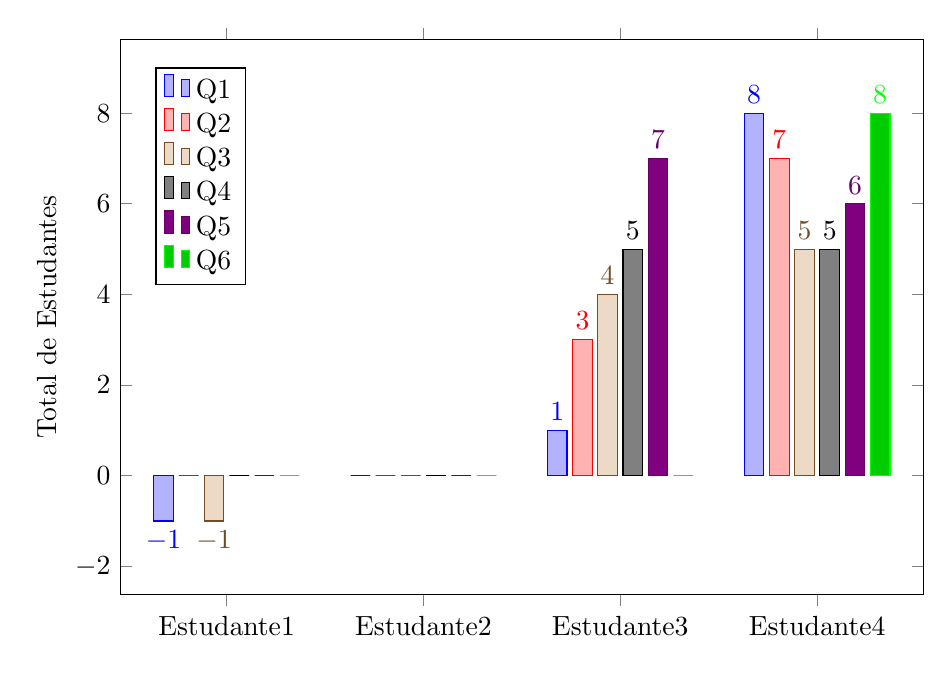
\begin{tikzpicture}[scale=1]
		\pgfplotsset{width=10cm,compat=newest}
		\begin{axis}[
		ybar,
		bar width=0.25cm,
		x=2.5cm,
		enlargelimits=0.18,
		legend style={at={(0.1,0.95)},
			anchor=north,legend columns=1},
		ylabel={Total de Estudantes
		},
		symbolic x coords={Estudante1, Estudante2, Estudante3, Estudante4},
		xtick=data,
		visualization depends on={y\as\YY},
		nodes near coords
		={\pgfmathtruncatemacro{\YY}{ifthenelse(\YY==0,0,1)}\ifnum\YY=0\else\pgfmathprintnumber\pgfplotspointmeta\fi},
		nodes near coords align={vertical},
		]
		
		\addplot+[] coordinates {
			% TS
			(Estudante1,-1) 
			(Estudante2,0) 
			(Estudante3,1) 
			(Estudante4,8)};
		
		\addplot+[] coordinates {
			% WS
			(Estudante1,0) 
			(Estudante2,0) 
			(Estudante3,3) 
			(Estudante4,7)};
		
		\addplot+[] coordinates {
			% AD
			(Estudante1,-1)
			(Estudante2,0) 
			(Estudante3,4)
			(Estudante4,5)};
		
		\addplot+[] coordinates {
			% QuCL
			(Estudante1,0)
			(Estudante2,0) 
			(Estudante3,5)
			(Estudante4,5)};
			
		\addplot+[] coordinates {
			% QuCL
			(Estudante1,0)
			(Estudante2,0) 
			(Estudante3,7)
			(Estudante4,6)};
			
		\addplot+[] coordinates {
			% QuCL
			(Estudante1,0)
			(Estudante2,0) 
			(Estudante3,0)
			(Estudante4,8)};
		\legend{Q1, Q2, Q3, Q4, Q5, Q6}
		\end{axis}
		\end{tikzpicture}
		\caption{Dúvida da Questão}
		\label{fig:DV}
	\end{figure}

\subsubsection{Grau de Assertividade}\label{sec:grau-assertividade}

\textbf{Grau de Assertividade ($A$)} é uma medida sobre a autoconfiança de um aluno ao responder a um conjunto de perguntas (que pode ser um questionário ou partes dele) com base na relação entre o número total de respostas corretas ($rc$ - consulte a Seção~\ref{sec:nota-tradicional}) e o somatório das marcações de resposta ($m_i$) em cada pergunta de um conjunto com $n$ questões. A Equação~\ref{eq:A} expressa a fórmula $A$ do grau de assertividade.

\begin{equation}
\label{eq:A}
A = \frac{rc}{\sum_{i=1}^{n} m_i}
\end{equation}

Por exemplo, dado um questionário de múltipla escolha, com três respostas possíveis, se um aluno escolheu a primeira alternativa, alterou sua resposta para a segunda alternativa e, depois, mudou novamente para a terceira alternativa antes de enviar a decisão final, podemos inferir que esse aluno não tinha certeza sobre sua escolha final. Isso pode ocorrer porque o aluno está confuso sobre os conceitos ou tem capacidade de autocorreção. No entanto, combinando $A$ com $NT$ (Nota Tradicional - ver Seção~\ref{sec:nota-tradicional}) ou $NCP$ (Nível de Compreensão do Questionário - ver Seção~\ref{sec:NC}), podemos observar os diferentes comportamentos dos alunos e, possivelmente, detectar quem teve mais dificuldades.

Além disso, existem alguns casos extremos a serem analisados para entender o potencial da assertividade ($A$). No primeiro caso, suponha que um aluno nunca mude suas respostas originais e obtenha a pontuação máxima ($rc=n$); portanto, seu ``grau de assertividade'' também é o \textit{máximo} ($A = 1$ ou $A = 100\%$). O segundo caso ocorre quando o aluno nunca muda suas respostas, mas todas estão erradas, indicando que ele interpretou os conceitos de uma maneira muito errada ($rc \approx 0 $ ou $ rc \ll n $); nesse caso, $A$ é mínimo ($A \approx 0$ ou $A \approx 0\%$). Finalmente, o terceiro caso caracteriza um comportamento menos problemático, em que o aluno altera suas respostas várias vezes ($\sum m_i > n$), mas a pontuação final mais próxima do máximo ($rc \approx n$), indicando capacidade de autocorreção ($0 \ll A < 1$). Esses casos ilustram as principais diferenças entre a análise simples da Nota Tradicional e o novo Grau de Assertividade.


\subsubsection{Tempo de Resposta}\label{section:Tempo}
Esta métrica calcula o tempo total que um estudante precisou para resolver cada questão ou um conjunto de questões (Figura~\ref{fig:exemplo_temporesposta_grafico}). A quantidade de tempo gasto na resolução de determinada questão pode dar indícios de que o estudante não compreendeu bem o assunto avaliado, a questão contém um nível de dificuldade muito elevado ou precisaria ser reformulada.

\begin{figure}[ht]
	\centering
	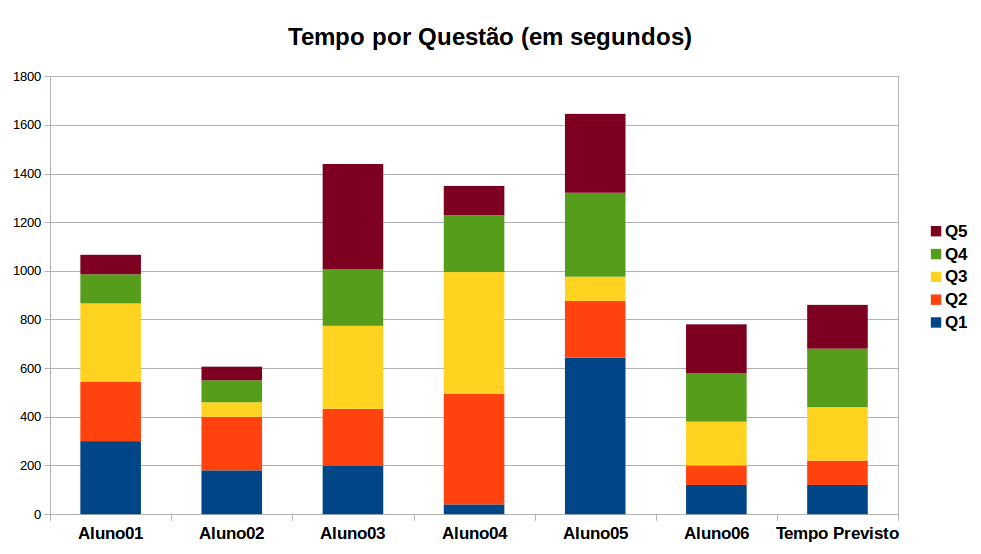
\includegraphics[width=0.8\linewidth]{chapters/proposedMethod/exemplo_tempo_questao}
	\caption{Exemplo do `Tempo de Resposta' de um Questionário (em segundos)}
	\label{fig:exemplo_temporesposta_grafico}
\end{figure}

Na Figura~\ref{fig:exemplo_temporesposta_grafico}, pode-se ainda realizar uma comparação entre o tempo de resposta de cada estudante com o estimado pelo professor no Compositor (veja Seção~\ref{section:composer}).

A medida do tempo de resposta do aluno ou da turma em uma questão (ou questionário) pode ser cruzada com o ``Grau de Assertividade'' (Seção~\ref{sec:grau-assertividade}), o que pode ajudar a visualizar a necessidade de maior reforço em algum conteúdo já estudado ou alguma recomendação de modificação da questão/questionário em si. Por exemplo, um baixo grau de assertividade da turma em uma determinada questão (classificada como `Fácil' pelo professor no Compositor) associada a um elevado tempo de resposta dessa mesma questão pode ser um indicativo de que a linguagem do problema precisaria ser revista ou os alunos não entenderam bem o tópico avaliado.

%\subsubsection{Nível de Desordem}\label{sec:disorder}
%
%O \textbf{Nível de Desordem ($D$)} é uma métrica que usa o conceito de entropia proveniente da área de teoria da informação, que ajuda a quantificar o grau de incerteza de uma variável aleatória ou o resultado de um processo aleatório~\citep{Mackay2003book}. Em outras palavras, a métrica $D$ representa o grau de desordem dos eventos gravados em um `\textit{log}' ou, mais precisamente, o quanto um estudante respondeu às questões em uma ordem diferente da originalmente proposta pelo professor.
%
%A entropia foi originalmente proposta por~\cite{Shannon1948} baseando-se na função massa de probabilidade, que associa uma probabilidade a cada possível ocorrência de uma variável aleatória discreta, tal como apresentado no trabalho de~\cite{bandt2002permutation} e expresso pela Equação~\ref{eq:H}:
%
%\begin{equation}\label{eq:H}
%H = -\sum_{i=1}^n p_i \log p_i
%\end{equation}
%
%\noindent onde $p_i$ é a probabilidade da ocorrência do \textit{i-ésimo} símbolo de um conjunto $N = \{1,2,\dots, n\}$. Um dos maiores problemas desta medida é como obter $p_i$ a partir de uma função distribuição de probabilidade desconhecida. Neste trabalho, nós consideramos apenas os símbolos $p_1$ e $p_2$, onde $p_1$ corresponde ao evento do aluno responder uma questão $t_i$ e, em seguida, responder uma questão $t_{i+1}$, sendo $p_2$ o evento inverso, isto é, responder uma questão $t_{i+1}$ seguida de uma questão $t_i$. Assim, podemos inferir $p_1$ e $p_2$ a partir da sequência de eventos como uma série temporal discreta.
%
%O pseudo-código do Algoritmo~\ref{algo:PE} mostra esta transformação baseada no trabalho original de~\cite{bandt2002permutation} chamado Entropia de Permutação. Assim, seja um questionário com 6 questões e um \textit{log} `$V$' com essas questões respondidas por um estudante e representado por $V = \{1,2,3,1,5,6,5,2,1,4\}$, o Nível de Desordem será calculado de acordo com os passos a seguir: 
%% percorrendo o vetor na ordem inversa afim de obter a ordem final das respostas, desconsiderando valores repetidos e aplicando . Neste caso, a ordem das respostas do estudante é dada por $V = \{3,6,5,2,1,4\}$. 
%
%\begin{enumerate}
% 	\item Extrair a sequência final das respostas, i.e.: $V'=\{3,6,5,2,1,4\}$;
%    \item Percorrer $V'$ comparando o número da resposta atual ($t_i$) com o número da resposta a seguinte ($t_{i+1}$). Toda vez que a condição $t_i \leq t_{i+1}$ for atendida, então, o contador $p_1$ deverá ser incrementado; caso contrário, é o contador $p_2$ que deverá ser incrementado;
%    \item Normalizar $p_1$ e $p_2$ para obter as probabilidades; e
%  \item Aplicar a Equação~\ref{eq:disorder}.
%\end{enumerate}
%
%\begin{algorithm}[!htb]
%% 	\scalefont{0.8}
%	\caption{Nível de Desordem} 
%	\label{algo:PE}
%	\SetAlgoLined
%	
%	\SetKwFunction{WriteLineCode}{WriteLineCode}
%	\SetKwFunction{GetValuesCEER}{GetValuesCEER}
%	\SetKwFunction{GetValuesCode}{GetValuesCode}
%	\SetKwFunction{GetTotalLineCE}{GetTotalLineCE}
%	\SetKwFunction{StartTrigger}{StartTrigger}
%	
%%	\KwIn{Code, CE\_Out}
%%	\KwOut{Novo código instanciado}                    
%%	\tcp{Primeira fase}
%
%    p1 = 0\; p2 = 0\;
%    \Para{$i=1$ to $n-1$}{
%    	\Se{$t_{i} \leq t_{i+1}$}{$p1++$}
%    	\Senao{$p2++$}
%     }
%    Calcular Equação~\ref{eq:disorder}
%\end{algorithm}
%
%    \begin{equation}\label{eq:disorder}
%    D = -\frac{p_1}{p_1+p_2} \ \log(\frac{p_1}{p_1+p_2})-\frac{p_2}{p_1+p_2} \ \log(\frac{p_2}{p_1+p_2})
%    \end{equation}
%
%Desse modo, a partir do Algoritmo~\ref{algo:PE}, obtemos os valores de $p_1=2$ e $p_2=3$ que serão utilizados na Equação~\ref{eq:disorder} e, para o exemplo em questão, o valor de $D$ é 0,6730. Vale ressaltar que quanto mais perto de `1', maior a desordem da resposta.
%
%A Figura~\ref{fig:exemplo_desordem_grafico} mostra o nível de desordem de estudantes de uma turma hipotética, onde se pode observar que alguns estudantes responderam o questionário de acordo com a ordem proposta pelo professor ($D=0$), enquanto outros responderam em uma ordem muito diferente ($D \approx 1$).
%
%\begin{figure}[ht]
%	\centering
%	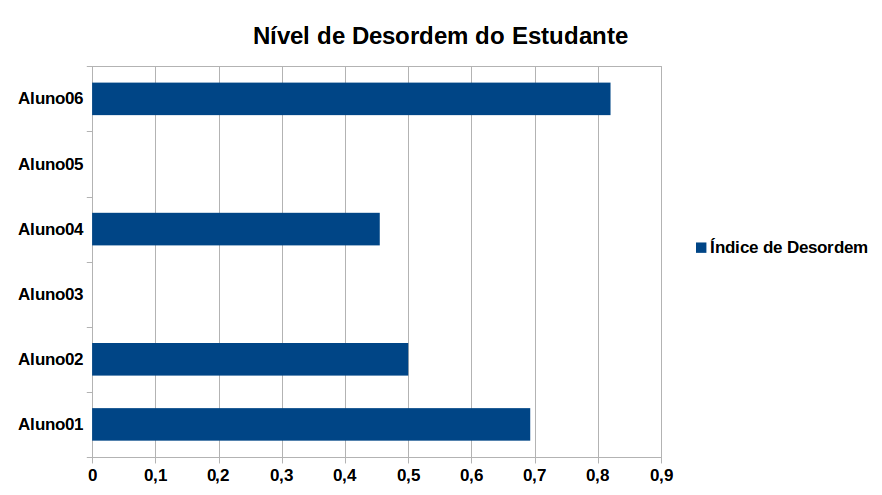
\includegraphics[width=0.8\linewidth]{imgs/exemplo_grafico_desordemv3}
%	\caption{Exemplo do Nível de Desordem por aluno}
%	\label{fig:exemplo_desordem_grafico}
%\end{figure}
%
%Esta métrica pode dar indícios do comportamento dos estudantes e ajudar a entender melhor o que pode estar acontecendo com os mesmos. Por exemplo, alunos com um alto nível de desordem podem ter mais dificuldades para responder um conjunto de questões do que outro. Nesse caso, essa métrica precisa ser associada a outras como o ``Desvio do Conjunto'' ou o ``Tempo de Resposta do Estudante'' para confirmar essa hipótese.

\subsection{Métricas Compostas}
As métricas apresentadas nesta subseção são consideraras compostas porque dependem de outras métricas para que sejam calculadas. 

%\subsubsection{Desvio do Conjunto}
%\label{sub:desvio-do-conjunto}
%
%Da mesma maneira que o Desvio da Resposta ($DR$), o \textbf {Desvio do Conjunto ($DC$)} representa a porcentagem da distância entre as respostas corretas e as respostas marcadas pelo aluno em um grupo de questões, por exemplo, um questionário. Em outras palavras, é o complementar da nota ponderada ($NP$). A equação ~\ref{eq:desvio} indica como calcular o desvio do conjunto para um aluno.
%
%\begin{equation}
%\label{eq:desvio}
%DC = (10 - NP) \cdot 10
%\end{equation}
%
%Ambas as métricas, NP e DC, são melhorias baseadas no parâmetro ``desvio'' do Nível de Entendimento (consulte a Seção~\ref{sec:level-understanding}). Nesse caso, DC significa a porcentagem do desvio real da resposta correta, diferente da proposta original de~\cite{Biswas:2007}, que indica que o valor do desvio cresce quando a resposta está mais próxima do valor correto.
%
%Por exemplo, aplicando a Equação~\ref{eq:desvio} nos dados da disciplina ``A'' da Tabela~\ref{tab:notas-estudantes}, podemos observar que, embora o aluno tenha $NT=6,67$, seu desvio de conjunto é de apenas $12,5\%$ devido ao valor de sua $NP=8,75$.
%%
%Na Disciplina ``B'', podemos observar que $NT=1,67$, o que indica uma alta quantidade de respostas incorretas. No entanto, o estudante tem $NP=7,92$ e seu Desvio do Conjunto é apenas de $20,8\%$. Assim, comparando PT e DC, em ambos os casos, é evidente que DC pode dizer com mais precisão sobre a aprendizagem dos alunos.

\subsubsection{Prioridade}
\label{sec:prioridade}

\textbf{Prioridade ($P$)} (veja Eq.~\ref{eq:prioridade}) indica a relevância de uma disciplina ou de um tópico a ser estudado por um aluno com base nas pontuações obtidas na Nota Tradicional ($NT$) e na Nota Ponderada ($NP$).
% Em outras palavras, a prioridade depende da relevância do tópico / assunto.

\begin{equation}
    \label{eq:prioridade}
    P = (10 - TS)\cdot \frac{WS}{10}
\end{equation}

Como apresentado anteriormente na Subseção~\ref{sec:nota-ponderada}, para a disciplina ``A'', temos $NT = 6,67 $ e $NP = 8,75$; e para a disciplina ``B'', $NT = 1,67 $ e $NP = 7,92$. Em seguida, podemos usar a Equação~\ref{eq:prioridade} para calcular a prioridade de cada assunto, resultando em:

$$ P_A = (10 - 6,67) \cdot \frac{8,75}{10} = 2,914$$
$$ P_B = (10 - 1,67) \cdot \frac{7,92}{10} = 6,597$$

Onde, a prioridade para a disciplina ``A'' é $2.914 $ e $6.597$ para a disciplina ``B''. Observando a Tabela~\ref{tab:notas-estudantes}, podemos ver que, apesar do melhor desempenho geral na Disciplina A, a Disciplina B tem mais prioridade e, portanto, é mais recomendável estudá-la primeiro. Isso acontece porque o aluno \textit{quase} acerta mais questões na Disciplina B, o que significa que é necessário um baixo nível de esforço para aprender e alcançar um alto desempenho.


\subsubsection{Nível de Compreensão da Questão}\label{sec:compreensao-questao}

O \textbf{Nível de Compreensão da Questão ($NCQ$)} mede o desempenho do aluno, levando em consideração o nível de dificuldade da questão e o tempo que levou para respondê-la. Portanto, o $NCQ$ é baseado no Índice de Dificuldade da Questão ($IDQ$) e no Índice de Dificuldade de Conteúdo ($IDC$) da Tabela~\ref{tab:DVI}, no peso ``p'' da resposta do aluno (ver Seção~\ref{sec:nota-ponderada} e Tabela~\ref{tab:Pesos}) e o Tempo de Resposta do estudante ($TR$). Assim, o nível máximo de compreensão ($Max$) é a maior compreensão possível de ser medida; e o Nível Efetivo de Compreensão ($NEC$) é a compreensão efetivamente medida, sendo obtidos pelas Equações~\ref{eq:MCL} e~\ref{eq:ECL}, respectivamente.

\begin{subequations}
\label{eq:MaxNEC}
\begin{equation}\label{eq:MCL}
Max = IDQ\cdot IDC \cdot 4
\end{equation}
\begin{equation}\label{eq:ECL}
NEC = IDQ \cdot IDC \cdot p
\end{equation}
\end{subequations}

Os valores de $IDQ$ e $IDC$ podem ser obtidos a partir da Tabela~\ref{tab:DVI}, onde `1' significa o conteúdo ou a pergunta com a menor dificuldade,`3' é considerado uma dificuldade normal e, finalmente, o valor '5' corresponde a um conceito mais difícil de entender.

\begin{table}[htbp]
\caption{Valores dos Índices de Dificuldade}
\begin{center}
\begin{tabular}{|c|c|c|c|}
\hline
\textbf{Índices} & \textbf{Fácil} & \textbf{Normal} & \textbf{Difícil}  \\ \hline
\textbf{Índice de Dificuldade da Questão - IDQ} & 1 & 3 & 5\\ \hline
\textbf{Índice de Dificuldade do Conteúdo - IDC} & 1 & 3 & 5\\ \hline
\end{tabular}
\end{center}
\label{tab:DVI}
\end{table}

Assim, $NCQ$ considera o tempo que o estudante levou para responder a questão e, de acordo com a Equação~\ref{eq:NCQ}, podemos ver que $NCQ$ pode ser calculado de três maneiras diferentes dependendo do tempo de resposta do aluno para cada pergunta. Além disso, a Tabela~\ref{tab:QCL_1st} demonstra cinco estudos de caso.

\begin{equation}
\fontsize{14}{14}\selectfont
\label{eq:NCQ}
NCQ = 
\begin{cases}
\frac{NEC}{Max\cdot 4}, & TR \leq t/4 \\
\frac{NEC}{Max}, & t/4 < TR \leq t\\
\frac{NEC}{Max + (\frac{TR - t}{t})}, & TR > t
\end{cases}
\end{equation}

onde $t$ é o tempo máximo esperado que o estudante leve para responder a questão.

Na Tabela~\ref{tab:QCL_1st}, podemos notar que Q1 implica que o aluno acertou a pergunta ($p_1 = 4$), mas respondeu muito rapidamente ($TR \leq t/4 \therefore 60 \leq 62,5$), o que pode indicar que ele tentou adivinhar (ou chutar) a resposta. Nesse caso, pela Equação~\ref{eq:NCQ}, o $NCQ$ será igual a apenas 25\%.

Por outro lado, Q2 e Q3 foram respondidas dentro do tempo esperado ($t/4 < TR \leq t$). Ou seja, ($62,5 <\textbf{70} \leq 250$) e ($45 < \textbf{60} \leq 180$), respectivamente.
No entanto, apenas o Q2 está totalmente correto, obtendo um $NCQ$ igual a 100\%. Q3 está quase correto e, portanto, seu $NCQ$ é de 75\%. Nesses casos específicos, podemos observar que o $NCQ$ do aluno depende apenas do peso de sua resposta.

\begin{table}[htbp]
\caption{Nível de Compreensão da Questão}
\centering
\begin{tabular}{|c|c|c|c|c|c|c|c|c|c|c|c|}
\hline
\multicolumn{2}{|c|}{\textbf{Questão}} & \multicolumn{2}{c|}{\textbf{Q1}} & \multicolumn{2}{c|}{\textbf{Q2}} & \multicolumn{2}{c|}{\textbf{Q3}} & \multicolumn{2}{c|}{\textbf{Q4}} & \multicolumn{2}{c|}{\textbf{Q5}} \\ \hline
\multicolumn{2}{|c|}{\textbf{p}} & \multicolumn{2}{c|}{4} & \multicolumn{2}{c|}{4} & \multicolumn{2}{c|}{3} & \multicolumn{2}{c|}{4} & \multicolumn{2}{c|}{2} \\ \hline
\textbf{IDC} & \textbf{IDQ} & 5 & 5 & 3 & 3 & 5 & 5 & 3 & 3 & 5 & 5 \\ \hline
\multicolumn{1}{|l|}{\textbf{NEC}} & \multicolumn{1}{l|}{\textbf{Max}} & \multicolumn{1}{l|}{100} & \multicolumn{1}{l|}{100} & \multicolumn{1}{l|}{36} & \multicolumn{1}{l|}{36} & \multicolumn{1}{l|}{75} & \multicolumn{1}{l|}{100} & \multicolumn{1}{l|}{36} & \multicolumn{1}{l|}{36} & 50 & 100 \\ \hline
\textbf{TR} & \textbf{t} & 60 & 250 & 70 & 250 & 60 & 180 & 300 & 250 & 650 & 300 \\ \hline
\multicolumn{2}{|c|}{\textbf{t/4}} & \multicolumn{2}{c|}{62,5} & \multicolumn{2}{c|}{62,5} & \multicolumn{2}{c|}{45} & \multicolumn{2}{c|}{62,5} & \multicolumn{2}{c|}{75} \\ \hline
\multicolumn{2}{|c|}{\textbf{NCQ}} & \multicolumn{2}{c|}{25\%} & \multicolumn{2}{c|}{100\%} & \multicolumn{2}{c|}{75\%} & \multicolumn{2}{c|}{99,45\%} & \multicolumn{2}{c|}{49,42\%} \\ \hline
\end{tabular}
\label{tab:QCL_1st}
\end{table}

No terceiro caso, a saber, quando o aluno exceder o tempo esperado ($TR > t \therefore \textbf{300} > 250$), será descontado um pequeno valor apenas para distingui-lo do segundo caso, independentemente de sua resposta. Portanto, se esse aluno atrasou mais do que o previsto, é provável que seu nível de compreensão seja apenas um pouco menor do que o nível de quem respondeu dentro do tempo esperado. Assim, embora o aluno tenha respondido corretamente a pergunta Q4, pela Equação~\ref{eq:NCQ}, seu $NCQ$ será 99,45\%.

Finalmente, o quinto caso mostra que o aluno também excedeu o tempo esperado ($SRT > t \therefore \textbf{650} > 300 $), mas, dessa vez, respondeu a pergunta incorretamente e, portanto, obteve um peso igual a 2. Assim, a pontuação do aluno será calculada de acordo com o terceiro caso da Equação~\ref{eq:NCQ} e será diminuída proporcionalmente ao tempo excedido e ao peso obtido, de modo que seu $NCQ$ dele será igual a 49,42\%.


\subsubsection{Nível de Compreensão do Questionário}\label{sec:NC}

Ao contrário da métrica $NCQ$, que é focada em questões isoladas, o Nível de Compreensão do Questionário ($NC$) mede o desempenho dos estudantes em um questionário (ou um conjunto de questões). Esta métrica é baseada no \textbf{$NCQ$} e no complementar do ``Grau de Assertividade'' ($1-A$) para cada questão. A Equação~\ref{eq:NC} detalha como calcular o $NC$, onde `n' é o total de questões.

\begin{equation}
\label{eq:NC}
NC = \frac{\sum_{i=1}^{n}NCQ_i}{n + (1 - A)}
\end{equation}

\begin{table}[htbp]
\caption{Nível de Compreensão do Questionário}
\centering
\begin{adjustbox}{center, width=\columnwidth-16pt}
\begin{tabular}{|c|c|c|c|c|c|c|}
\hline
\multicolumn{7}{|c|}{\textbf{Disciplina A}} \\ \hline
\textbf{Questão} & \textbf{Q1} & \textbf{Q2} & \textbf{Q3} & \textbf{Q4} & \textbf{Q5} & \textbf{Q6} \\ \hline
\textbf{NCQ} & 1 & 0,75 & 1 & 0,50 & 1 & 1 \\ \hline
\textbf{1-A} & \multicolumn{6}{c|}{0,764} \\ \hline
\multicolumn{7}{|c|}{\textbf{Disciplina B}} \\ \hline
\textbf{Questão} & \textbf{Q1} & \textbf{Q2} & \textbf{Q3} & \textbf{Q4} & \textbf{Q5} & \textbf{Q6} \\ \hline
\textbf{NCQ} & 0,75 & 0,75 & 0,75 & 0,75 & 0,75 & 1 \\ \hline
\textbf{1-A} & \multicolumn{6}{c|}{0,833} \\ \hline
\end{tabular}
\end{adjustbox}
\label{tab:NC}
\end{table}

Através da Equação~\ref{eq:NC} e usando os dados da Tabela~\ref{tab:NC}, podemos calcular o $NC$, contendo as mesmas perguntas e respostas relacionadas às disciplinas `A' e `B' na Seção~\ref{sec:nota-ponderada} (Tabela~\ref{tab:notas-estudantes}:

$$NC_A = \frac{1 + 0,75 + 1 + 0,50 + 1 + 1}{6 + 0,764} \approx 77,61\% $$

$$NC_B = \frac{0,75 + 0,75 + 0,75 + 0,75 + 1}{6 + 0,833} \approx 58,54\% $$

No caso da disciplina `A', enquanto $NT_A = 6,67$ e $NP_A = 8,75$, $NC_A = 77,61\%$, e, no caso da disciplina `B', enquanto $NT_B=1,67$ e $NP_B=7,92$, tem-se um $NC_B=58,54\%$, onde estamos levando em consideração não apenas os pesos, acertos ou erros, mas também os índices de dificuldade de cada questão. Além disso, podemos notar que essa métrica usa elementos de quase todas as métricas definidas anteriormente e, assim, pode falar sobre o entendimento do estudante com mais propriedade do que a Nota Tradicional ($NT$).

\subsection{Métricas aplicadas a Objetos Tangíveis de Aprendizagem (OTA)}\label{subsec:aplicacao_metricasOFVA}

Embora as métricas apresentadas neste trabalho tenham sido inicialmente propostas e validadas com base em questionários de múltipla-escolha, uma vez que elas são produto do aprimoramento das métricas apresentadas por~\cite{leitao:2017}, propomos a sua extrapolação, e consequente utilização, para avaliação da aprendizagem a partir do uso de Objetos Tangíveis de Aprendizagem. 

\begin{figure}[htb]
	\centering
	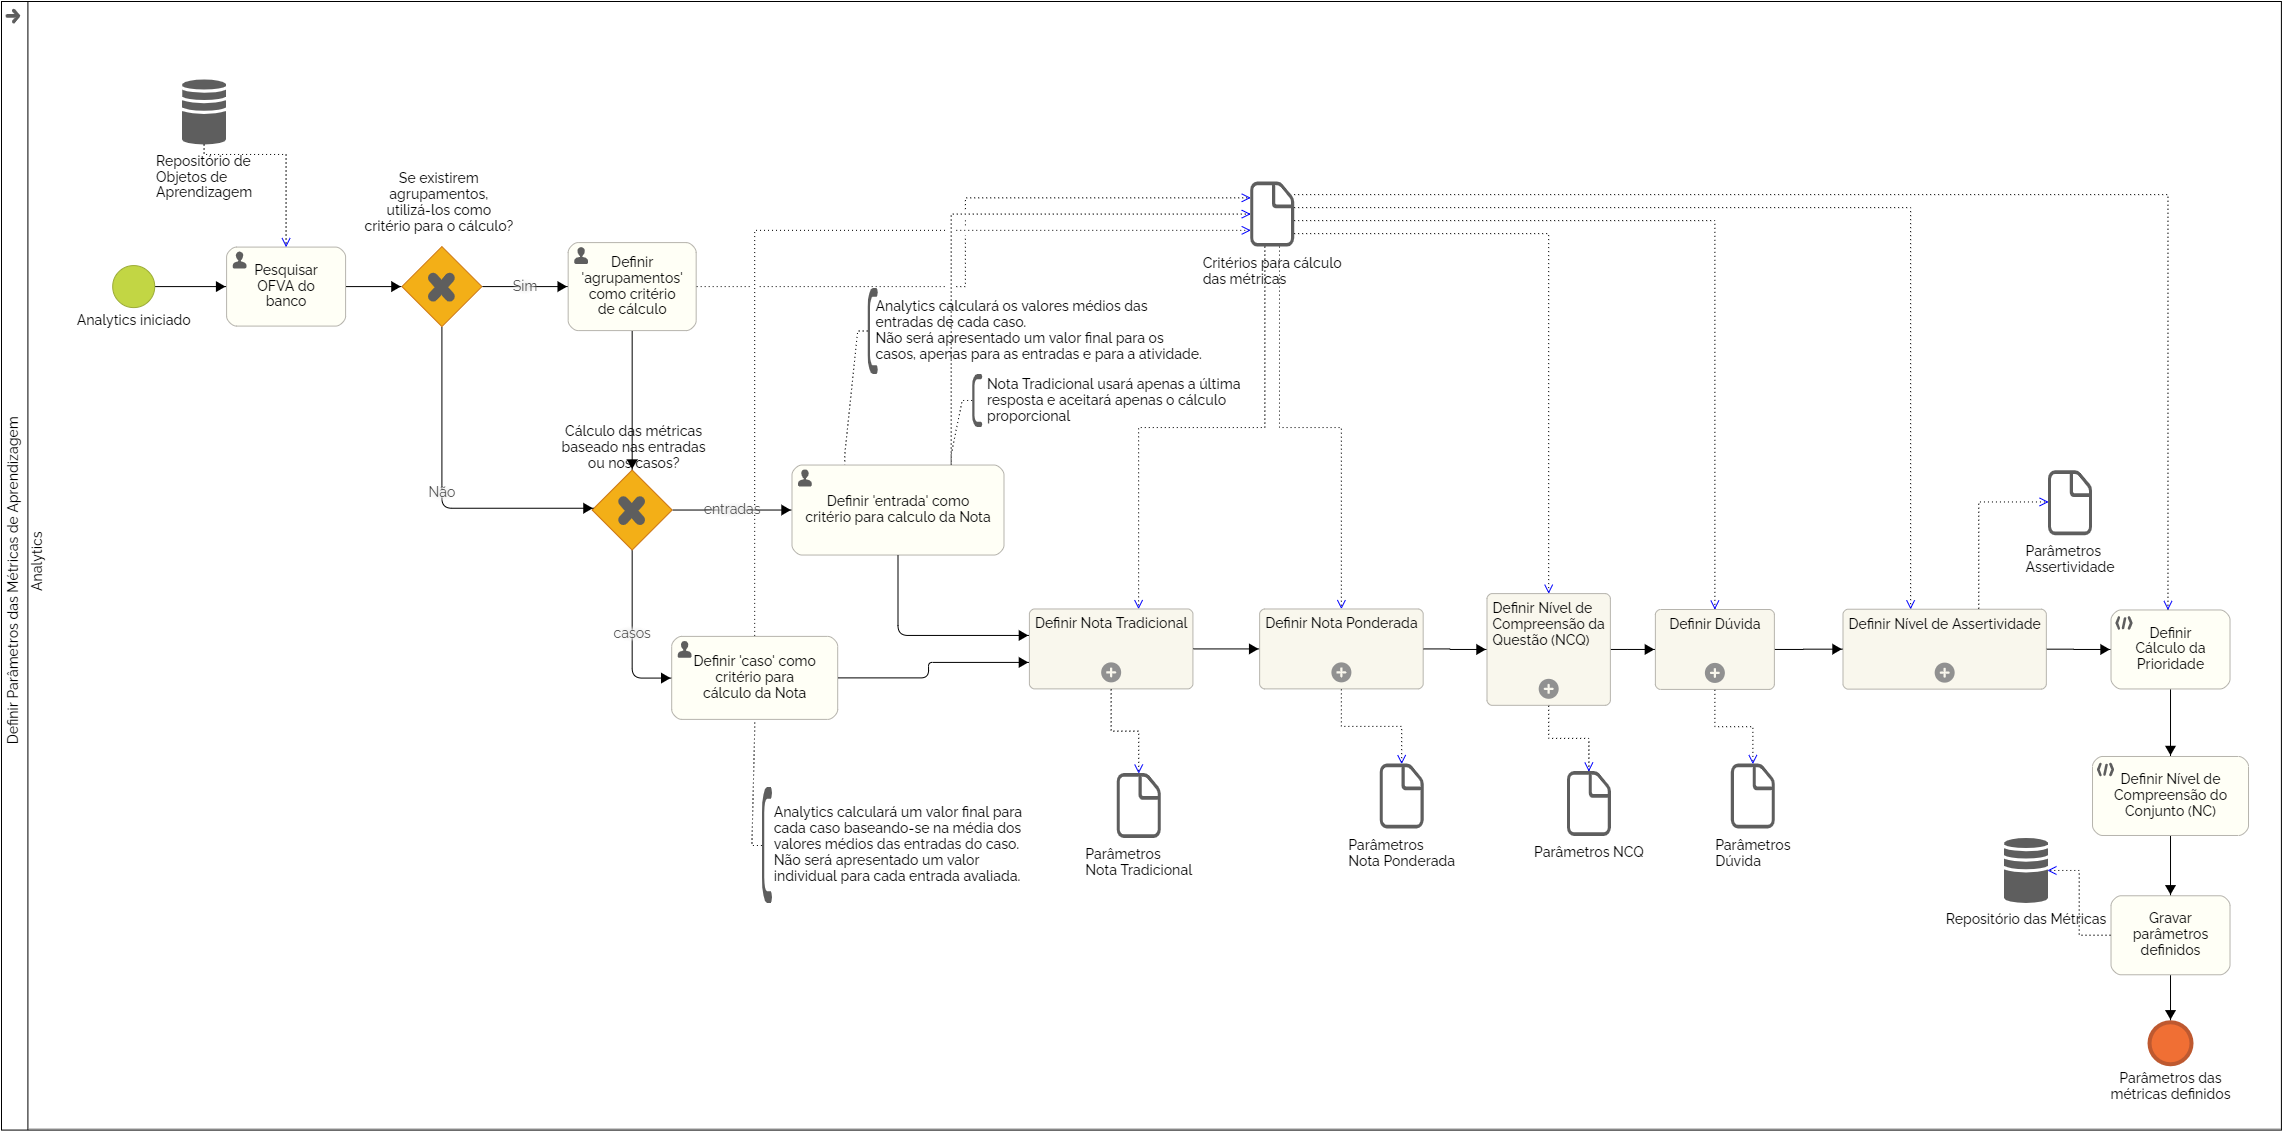
\includegraphics[width=1\linewidth]{chapters/proposedMethod/bpmn_metricas.png}
	\caption{Diagrama BPMN para Definição dos Parâmetros das Métricas de Aprendizagem aplicadas a um OTA}
	\label{fig:bpmn_metricas}
\end{figure}

Assim, de modo a conduzir a aplicação das métricas propostas aos objetos tangíveis utilizados em conjunto com a abordagem proposta nas seções anteriores, um modelo de processos BPMN é apresentado na Figura~\ref{fig:bpmn_metricas}.

\begin{figure}[htb]
	\centering
	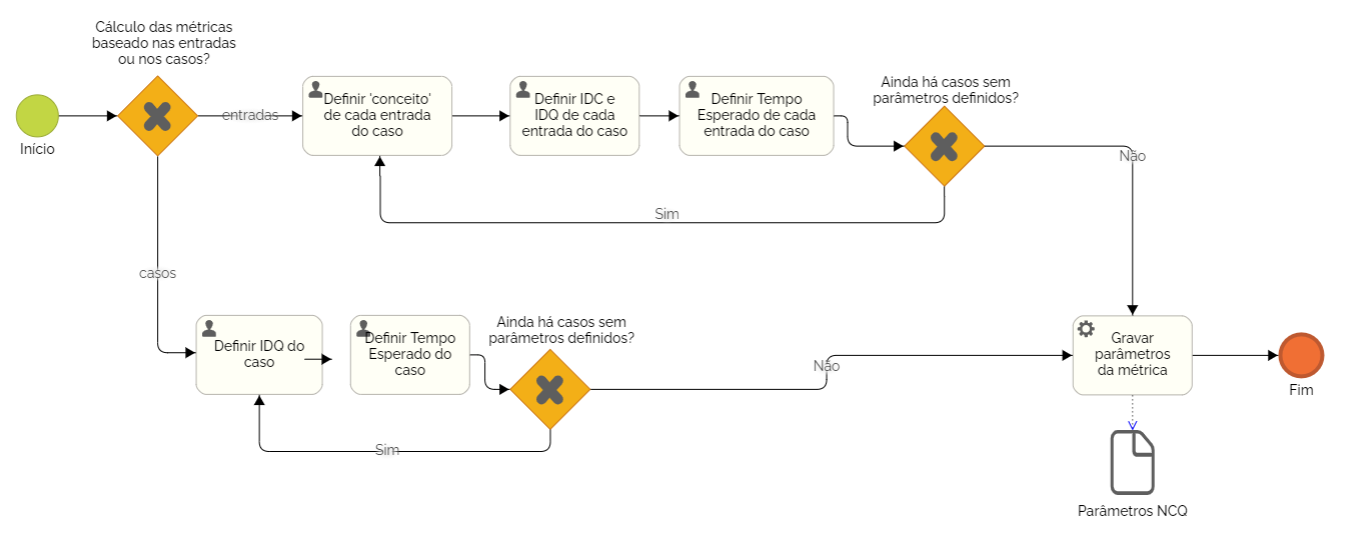
\includegraphics[width=0.9\linewidth]{chapters/proposedMethod/bpmn_metricas_NCQ.png}
	\caption{Subprocesso para definição dos parâmetros do Nível de Compreensão da Questão}
	\label{fig:bpmn_metricas_NCQ}
\end{figure}

Enquanto a Figura~\ref{fig:bpmn_metricas} apresenta o modelo geral do processo para caracterização das métricas de aprendizagem de cada objeto tangível, a Figura~\ref{fig:bpmn_metricas_NCQ} detalha os passos necessários para a parametrização do Nível de Compreensão da Questão (NCQ), que depende dos índices de dificuldade e do tempo esperado/gasto em cada caso de teste.

Assim, pode-se notar que há duas possibilidades a seguir para o cálculo da pontuação do estudante: (i) baseado nas entradas ou (ii) baseado nos casos de teste. Caso a primeira opção seja a escolhida, então, módulo Analíticos irá calcular o $NCQ$ tomando como base as entradas de todos os casos de teste e a nota gerada dependerá também dos índices de dificuldade do conteúdo e da entrada além do tempo de resposta esperado específicos de cada entrada.

Caso a segunda opção seja a escolhida, então, a nota será calculada tomando como base cada caso de teste com seus respectivos parâmetros.

\begin{figure}[htb]
	\centering
	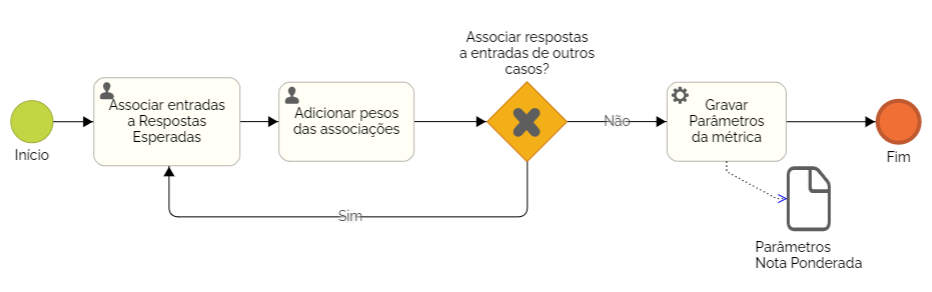
\includegraphics[width=0.9\linewidth]{chapters/proposedMethod/bpmn_metricas_NP.png}
	\caption{Subprocesso para definição dos parâmetros da Nota Ponderada}
	\label{fig:bpmn_metricas_NP}
\end{figure}

A Figura~\ref{fig:bpmn_metricas_NP} evidencia a necessidade de indicar os pesos para as diversas possibilidades de respostas dadas pelos estudantes, o que viabiliza o cálculo da Nota Ponderada %e do Desvio da Resposta e, por conseguinte, do NCQ.
e, por conseguinte, do NCQ. Além disso, a Figura~\ref{fig:CASO1NPEF1} apresenta a associação entre uma entrada ($EF1$) a um caso de teste (``Caso de Teste 1'') com as respectivas respostas esperadas ($RE$) e os pesos de cada resposta.

\begin{figure}[htb]
	\centering
	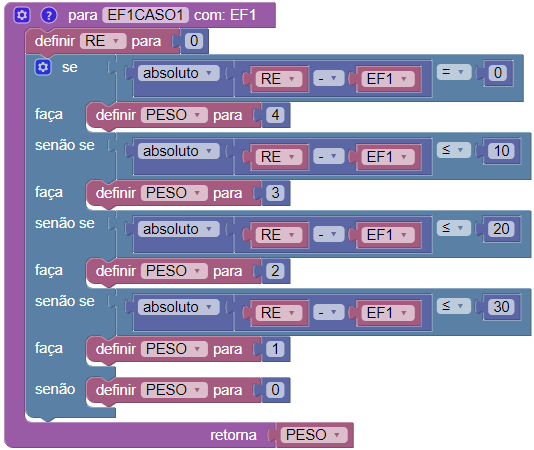
\includegraphics[width=0.6\linewidth]{chapters/appendixAnalytics/CASO1NPEF1.png}
	\caption{Exemplo de definição da NP para EF1 do Caso de Teste 1}
	\label{fig:CASO1NPEF1}
\end{figure}

Adicionalmente, também foram definidos subprocessos para a Nota Tradicional (Figura~\ref{fig:bpmn_metricas_NT}), Dúvida (Figura~\ref{fig:bpmn_metricas_Duvida}) e Assertividade (Figura~\ref{fig:bpmn_metricas_NA}) de modo a melhor caracterizar o fluxo e os parâmetros de cada uma dessas métricas.

\begin{figure}[htb]
	\centering
	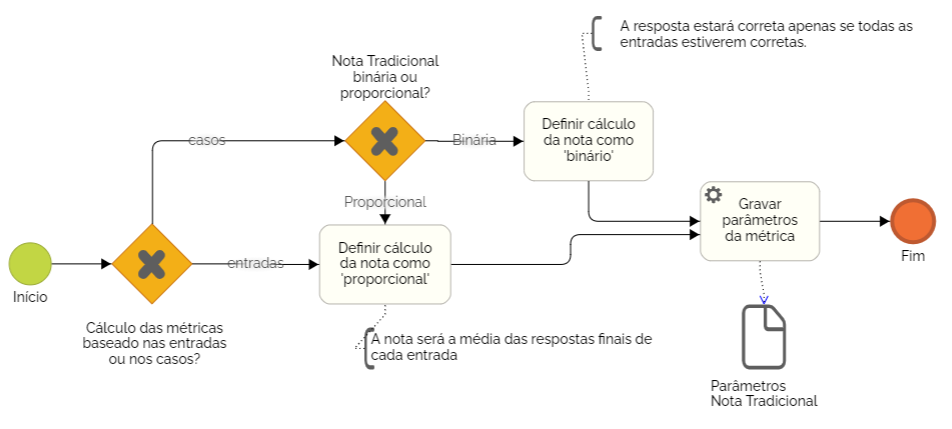
\includegraphics[width=0.9\linewidth]{chapters/proposedMethod/bpmn_metricas_NT.png}
	\caption{Subprocesso para definição dos parâmetros da Nota Tradicional}
	\label{fig:bpmn_metricas_NT}
\end{figure}

Por fim, foi realizado um estudo de caso (ver Seção~\ref{sec:estudo_caso1}) com o objetivo de validar e aprimorar o método apresentado neste trabalho. Tal estudo de caso consiste na implementação e utilização de objetos tangíveis de aprendizagem baseados no método proposto que instanciam o manipulativo físico-digital ``Quadro Trigonométrico'' e proveem dados e analíticos de aprendizagem. Além disso, as atividades pedagógicas nas quais as instâncias do OTA serão utilizadas estão baseadas em uma sequência didática proposta por~\cite{silva:2011} para o ensino de trigonometria. 

\begin{figure}[htb]
	\centering
	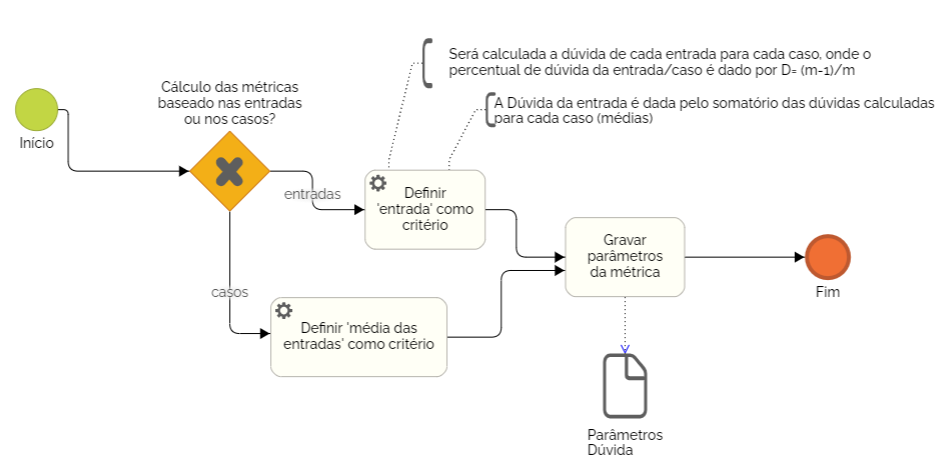
\includegraphics[width=0.9\linewidth]{chapters/proposedMethod/bpmn_metricas_Duvida.png}
	\caption{Subprocesso para definição dos parâmetros da Dúvida}
	\label{fig:bpmn_metricas_Duvida}
\end{figure}

Essa sequência prevê uma dinâmica construtivista para o estudo das relações e razões trigonométricas, sendo que cada atividade pedagógica tem por objetivo introduzir uma parte do círculo trigonométrico, de modo que, ao final da sequência, o estudante tenha construído conhecimento acerca dos quadrantes, posição dos ângulos em uma circunferência, valores destes ângulos em graus e radianos, além dos valores de seno, cosseno e tangente de cada ângulo.

\begin{figure}[htb]
	\centering
	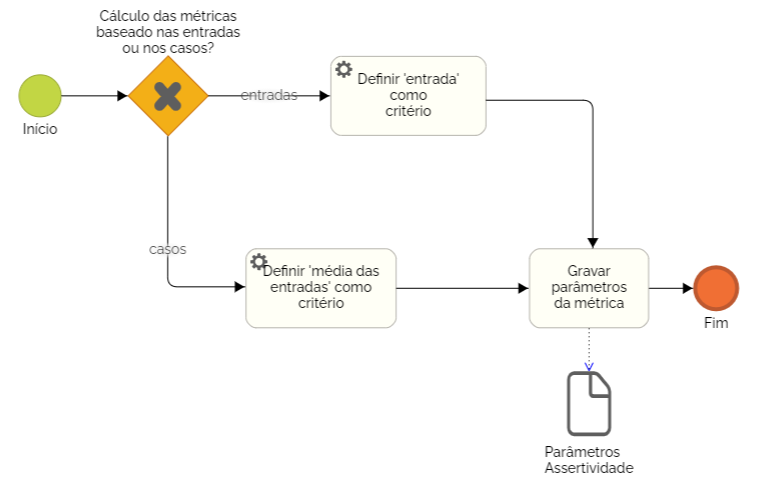
\includegraphics[width=0.8\linewidth]{chapters/proposedMethod/bpmn_metricas_NA.png}
	\caption{Subprocesso para definição dos parâmetros da Assertividade}
	\label{fig:bpmn_metricas_NA}
\end{figure}

\section{Ferramentas}\label{section:Tools}

Esta seção descreve brevemente as ferramentas implementadas para a validação do método proposto nesta tese. Tais ferramentas serão descritas seguindo cada parte do método apresentado ao longo deste capítulo.

 \begin{figure}[htb]
	\centering
	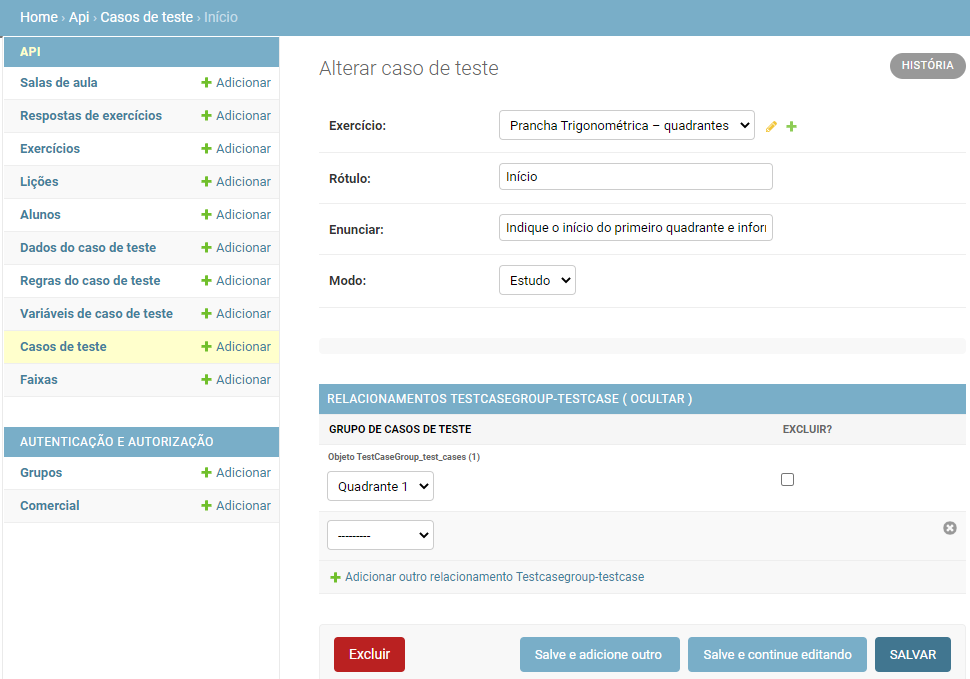
\includegraphics[width=0.95\linewidth]{chapters/proposedMethod/tools/composer_ota}
	\caption{Compositor de OTA - Casos de Teste}
	\label{fig:composer_ofva_testcase}
\end{figure}

\subsection{Compositor}

%O Compositor é uma ferramenta web desenvolvida usando o nodejs, os \textit{Frameworks} Angular e Django, associados a um banco de dados SQL. O componente em Angular corresponde a atualização da versão apresentada por~\cite{leitao:2017} de modo a prover melhores recursos e experiência ao usuário, tendo tido a interface proposta por uma aluna do curso de Design da UFAM. Já o componente em Django, viabiliza a inclusão dos objetos físico-virtuais de aprendizagem de acordo com o modelo de processos apresentado nas Figuras~\ref{fig:bpmn_ofva} e~\ref{fig:bpmn_ofva_casos}.

O Compositor é uma ferramenta web desenvolvida usando o nodejs, o \textit{Framework} Angular associado a um banco de dados SQL e uma versão modificada da Ferramenta Blockly. Com Angular, foram implementados dois componentes em separado, de modo que o primeiro corresponde a atualização da versão apresentada por~\cite{leitao:2017} de modo a prover melhores recursos e experiência ao usuário, tendo tido a interface proposta por uma aluna do curso de Design da UFAM. Já o segundo componente, viabiliza a inclusão dos objetos tangíveis de aprendizagem de acordo com o modelo de processos apresentado nas Figuras~\ref{fig:bpmn_ofva} e~\ref{fig:bpmn_ofva_casos}.

A Figura~\ref{fig:composer_ofva_testcase} apresenta uma imagem da tela de inserção dos casos de teste utilizados na instanciação do objeto tangível utilizado neste trabalho. Note-se que é possível editar o Rótulo, o Enunciado, o modo de utilização do estudante (Estudo ou Avaliação) e, por fim, o agrupamento ao qual o caso de teste pode estar vinculado.

 \begin{figure}[htb]
	\centering
	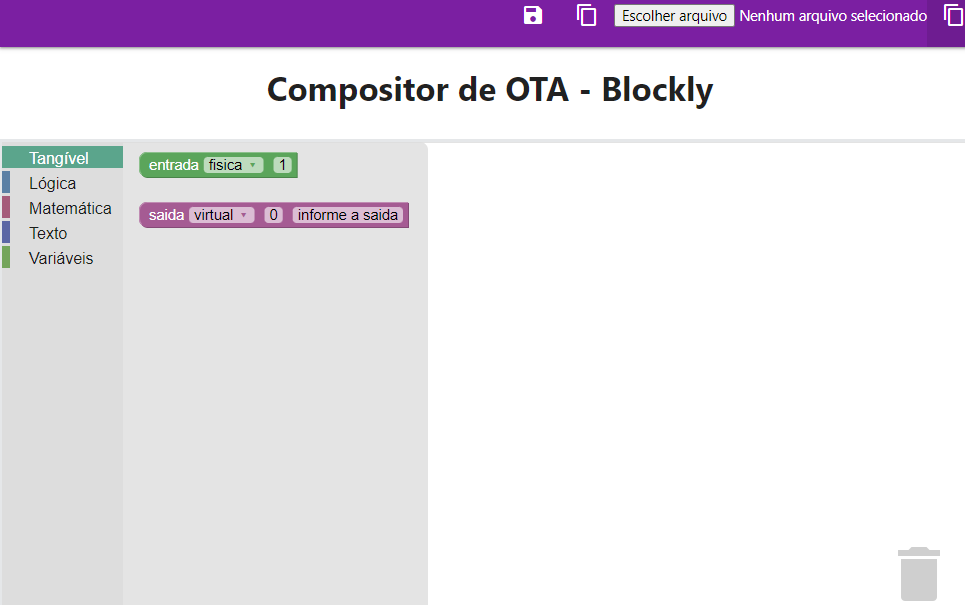
\includegraphics[width=0.95\linewidth]{chapters/proposedMethod/tools/blockly_ota}
	\caption{Compositor de OTA - Blockly}
	\label{fig:composer_ofvablockly}
\end{figure}

Como dito anteriormente, para definição das variáveis de entrada e saída e das regras de validação dos casos de teste, foi implementada uma ferramenta de programação em blocos baseada na biblioteca de código aberto Blockly~\citep{Blockly:2022}, mantida pelo Google. A Figura~\ref{fig:composer_ofvablockly} apresenta a tela principal da ferramenta modificada e que permite a utilização de blocos específicos para a necessidade do Compositor de Objetos Tangíveis, de modo que esses blocos podem ser salvos para reutilização e o código-fonte seja automaticamente traduzido para JavaScript, que é a linguagem utilizada pelo Player para validação das respostas dos estudantes.

Dentre as modificações implementadas estão a possibilidade de declarar e editar as entradas e saídas tangíveis (físicas e virtuais), a abertura e o salvamento dos blocos utilizados em um arquivo xml de modo a permitir edições posteriores, o salvamento do código gerado automaticamente em java script de modo que possa ser exportado e armazenado em um banco de dados SQL.

% % Ao iniciar o Compositor, é exibida uma página com informações gerais sobre os componentes relacionados a criação e condução da Aula Digital, isto é, o Compositor, o Player e o Servidor (Figura~\ref{fig:composer_telainicial}).

% \begin{figure}[htb]
% 	\centering
% 	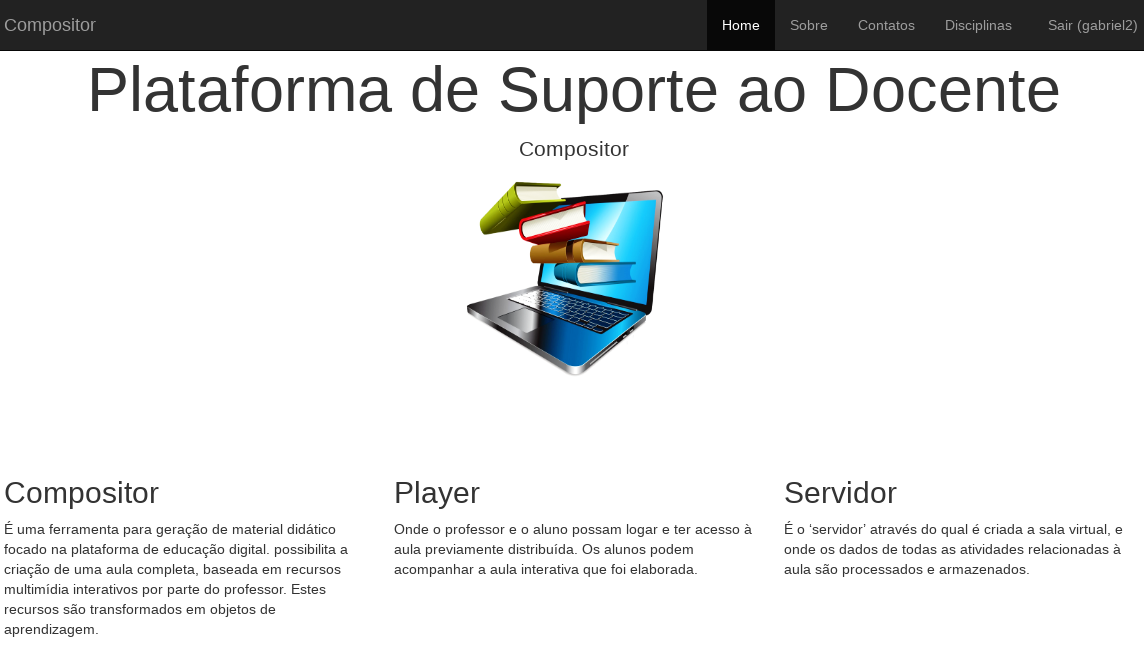
\includegraphics[width=0.95\linewidth]{imgs/tools/composer_telainicial}
% 	\caption{Tela Inicial do Compositor}
% 	\label{fig:composer_telainicial}
% \end{figure}

% % Através da interface apresentada na Figura~\ref{fig:compositor_disciplinas}, é possível criar novas disciplinas ou gerenciar disciplinas já existentes no banco de dados. Após criar uma disciplina, é possível criar ou gerenciar as Aulas relacionadas a ela e, para cada aula, criar ou gerenciar o Capítulo (Tópico) a ser trabalhado, conforme introduzido na Seção~\ref{section:composer}.

% \begin{figure}[htb]
% 	\centering
% 	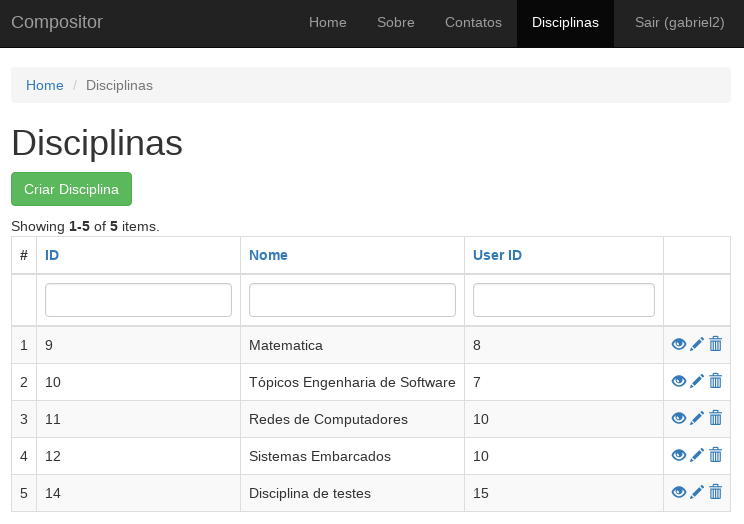
\includegraphics[width=0.9\linewidth]{imgs/tools/compositor_disciplinas}
% 	\caption{Compositor - Tela `Disciplinas'}
% 	\label{fig:compositor_disciplinas}
% \end{figure}

% % Cada Objeto de Aprendizagem é vinculado a um Capítulo, assim, a Figura~\ref{fig:compositor_objetosaprendizagem} apresenta a tela do Compositor relativa ao Capítulo sobre `Comutação e Roteamento' da Disciplina `Redes de Computadores', onde é possível verificar a existência dos OAs `Galeria', `Vídeo', `Apresentação' e `Questionário'. Além disso, nesta mesma tela, é feita a identificação do nível de dificuldade o Tópico, a ser utilizado nas métricas de avaliação do estudante (Seção~\ref{section:analytics}).

% % \begin{figure}[ht]
% % 	\centering
% % 	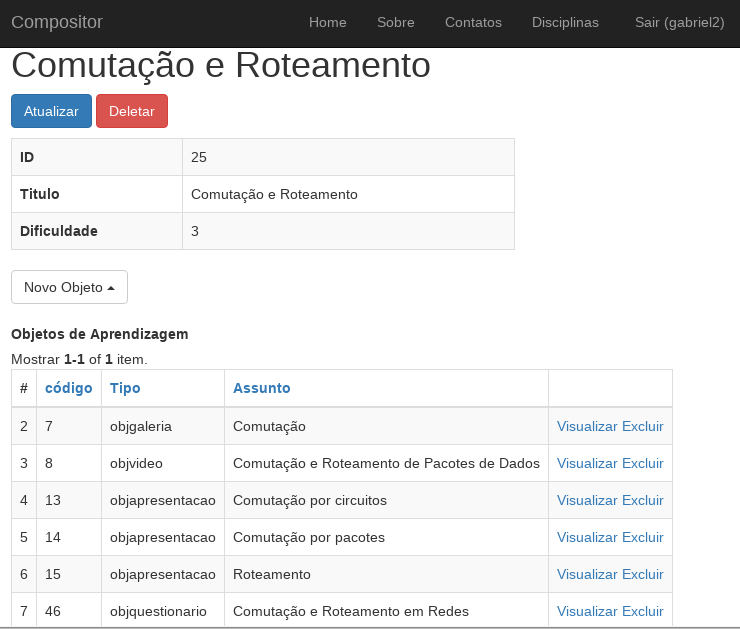
\includegraphics[width=0.75\linewidth]{imgs/tools/compositor_objetosaprendizagem}
% % 	\caption{Compositor - Tela `Objetos de Aprendizagem'}
% % 	\label{fig:compositor_objetosaprendizagem}
% % \end{figure}

% % Somente após a criação ou inserção dos objetos de aprendizagem específicos de um capítulo, são executados \textit{scripts} para a geração do conjunto de páginas web que farão a composição da Aula Digital a ser executada pelo Player.

% \subsection{Objetos Físico-Virtuais de Aprendizagem}

\subsection{Player Tangível}\label{subsec:tools_player}

O `Player' é o módulo onde acontece a interação do aluno com o conteúdo educacional. No caso de objetos de aprendizagem tradicionais, tal interação é essencialmente digital de modo que o estudante tem acesso e interage com o objeto de aprendizagem exclusivamente através de algum dispositivo tradicional (computadores, \textit{smartphones}, \textit{tablets},...). Entretanto, no caso de objetos tangíveis, a interação com o material pedagógico acontece também através de um manipulativo físico que tem uma contraparte digital. Assim, nesta subseção, apresentaremos uma instância de um OTA criado para a prova de conceito desta tese.

% % Além disso, através de um \textit{Javascript} chamado ``DataCollector'', o Player coleta todos os dados de interação do estudante com o material didático exibido por ele. Esses dados são enviados para o servidor para análise da dificuldade do estudante para ativação das ajudas sob demanda (Figura~\ref{fig:player_adaptacao}), criação do \textit{log} da aula e posterior análise pelas métricas. Assim, a Figura~\ref{fig:player_adaptacao} apresenta a tela do Player utilizada na `Aula 01', uma das aulas apresentadas no Capítulo~\ref{Chap:partialResults} (Seção~\ref{subsection:questionarioAula01}). 

% % \begin{figure}[ht]
% % 	\centering
% % 	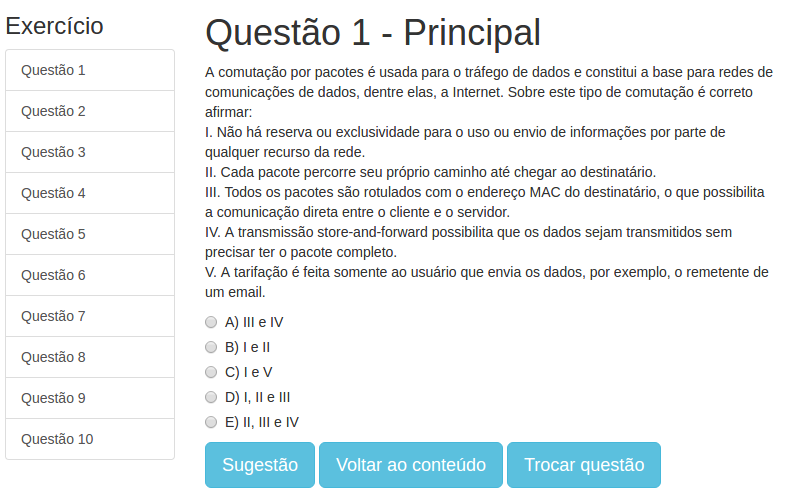
\includegraphics[width=0.95\linewidth]{imgs/tools/player_adaptacao}
% % 	\caption{Player - Questionário com Ajuda sob Demanda}
% % 	\label{fig:player_adaptacao}
% % \end{figure}

% Assim, com o objetivo de validar método e a arquitetura propostas nesta Tese, foi executado um estudo de caso para o qual foi proposto e implementado um objeto de aprendizagem físico-virtual de acordo com as especificações definidas na Seção~\ref{section:OA_fisicovirtual}. Desse modo, a Tabela~\ref{tabela:OFV_estudo_caso1} apresenta uma instanciação de um OFV chamado ``Quadro Trigonométrico''. Tal objeto tem por objetivo facilitar e verificar a aprendizagem de estudantes do Ensino Médio, no que diz respeito aos tópicos Trigonometria, Ângulos, Graus, Radianos e Razões Trigonométricas (seno, cosseno e tangente).

\begin{table}[htb]
	\caption{Aspectos Educacionais: Prancha Trigonométrica - Quadrantes}
	\centering
	\begin{tabular}{|l|l|}
		\hline
		\textbf{Atributo} & \textbf{Descrição} \\ \hline
		\textbf{ID} & 001 \\ \hline
		\textbf{Título} & Prancha Trigonométrica: Quadrantes \\ \hline
		\textbf{Descrição Geral} & \begin{tabular}[c]{@{}l@{}}Este objeto de aprendizagem trabalha com conceitos relacionados a \\Trigonometria, em especial, os valores dos quadrantes do círculo \\trigonométrico.\end{tabular} \\ \hline
		\textbf{Descrição Educacional} & \begin{tabular}[c]{@{}l@{}}Na Interface Virtual, o estudante deve escolher o item a ser estudado \\(início ou fim de um quadrante) e, então, deve manipular o ponteiro \\da Interface Física de modo a indicar a posição (ângulo) em que o \\quadrante começa ou termina (de acordo com o item escolhido). 
			\\Para cada movimentação do ponteiro físico, o ponteiro virtual é \\movimentado e, após a confirmação da posição pelo estudante, é \\habilitada uma caixa de texto, onde deverão ser inseridos os valores \\do ângulo em graus e em radianos. Caso o aluno posicione o \\ponteiro físico em um local que não é um limite de quadrante, ou \\insira um valor incorreto, a Interface Virtual deverá retornar uma \\informação que o ajude a corrigir os valores ou posições. \\Este objeto deve usar a Face A01.\end{tabular} \\ \hline
		\textbf{Tópicos} & \begin{tabular}[c]{@{}l@{}}Trigonometria, ângulos, círculo trigonométrico, quadrantes, graus, \\radianos.\end{tabular} \\ \hline
		\textbf{Modo} & Estudo \\ \hline
		\textbf{Gateway} & .hex e .ino em Arduíno \\ \hline
		\textbf{Dispositivos} & \begin{tabular}[c]{@{}l@{}} 32 Sensores de efeito Hall; 1 teclado membrana; matricial;\end{tabular} \\ \hline
		
		%\textbf{Recursos Físicos} & \begin{tabular}[c]{@{}l@{}}.hex e .ino em Arduíno, Ponteiro físico, Face A01 (com círculo \\trigonométrico sem posições/valores de ângulos/quadrantes \\definidos)\end{tabular} \\ \hline
		%\textbf{Recursos Digitais} & Player Virtual \\ \hline
		%\textbf{Serviços} & \begin{tabular}[c]{@{}l@{}}Iniciar atividade (botão); Leitura de hipertexto; Envio de resposta \\física (botão físico + formato: json + requisição websocket); Envio \\de resposta digital (html \textit{tracking}); Confirmação de resposta \\(visualização de respostas dadas); \textit{Feedback} (modo estudo); \\Encerrar atividade (botão)\end{tabular} \\ \hline
		%% \textbf{Casos de Teste} & \begin{tabular}[c]{@{}l@{}}Situação 1: Maria tinha 2 lápis de cor. Ela ganhou mais 3. Quantos \\lápis Maria tem agora?; \\Entrada Física: 2 + 3; Entrada Digital: 5(4), 4(3), 6(3), 3(2), 7(2);\\ \\Situação 2: Mariana tem 2 borrachas e ganhou mais 2. \\Com quantas borrachas Mariana ficou?; \\Entrada Física: 2 + 2; Entrada Digital: 4(4), 3(3), 5(3), 2(2), 6(2);\\ \\IDQ: 1 IDC: 1 TR: 200s\end{tabular} \\ \hline
	\end{tabular}
	\label{tabela:OFV_estudo_caso1}
\end{table}

\subsubsection{Instanciação da descrição de um Objeto Tangível de Aprendizagem}\label{subsubsec:descricaoOFVA}
Tomando por base o perfil de aplicação OBAA escolhido (disponível no Apêndice~\ref{Chap:AppendixA}) e a Tabela~\ref{tabela:OFV}, que resume as especificações para criação de um OTA conforme o proposto nesta pesquisa, com o objetivo de validar o método e a arquitetura propostas nesta tese, foram implementados cinco OTAs. % de acordo com as especificações definidas na Seção~\ref{section:OA_fisicovirtual}.
E, como afirmado na Seção~\ref{subsec:aplicacao_metricasOFVA}, tais objetos tangíveis são baseados nas atividades pedagógicas da sequência didática proposta por~\cite{silva:2011}, de modo que cada objeto representa uma parte da construção do ``Quadro Trigonométrico'' final.

\begin{figure}[htb]
	\centering
	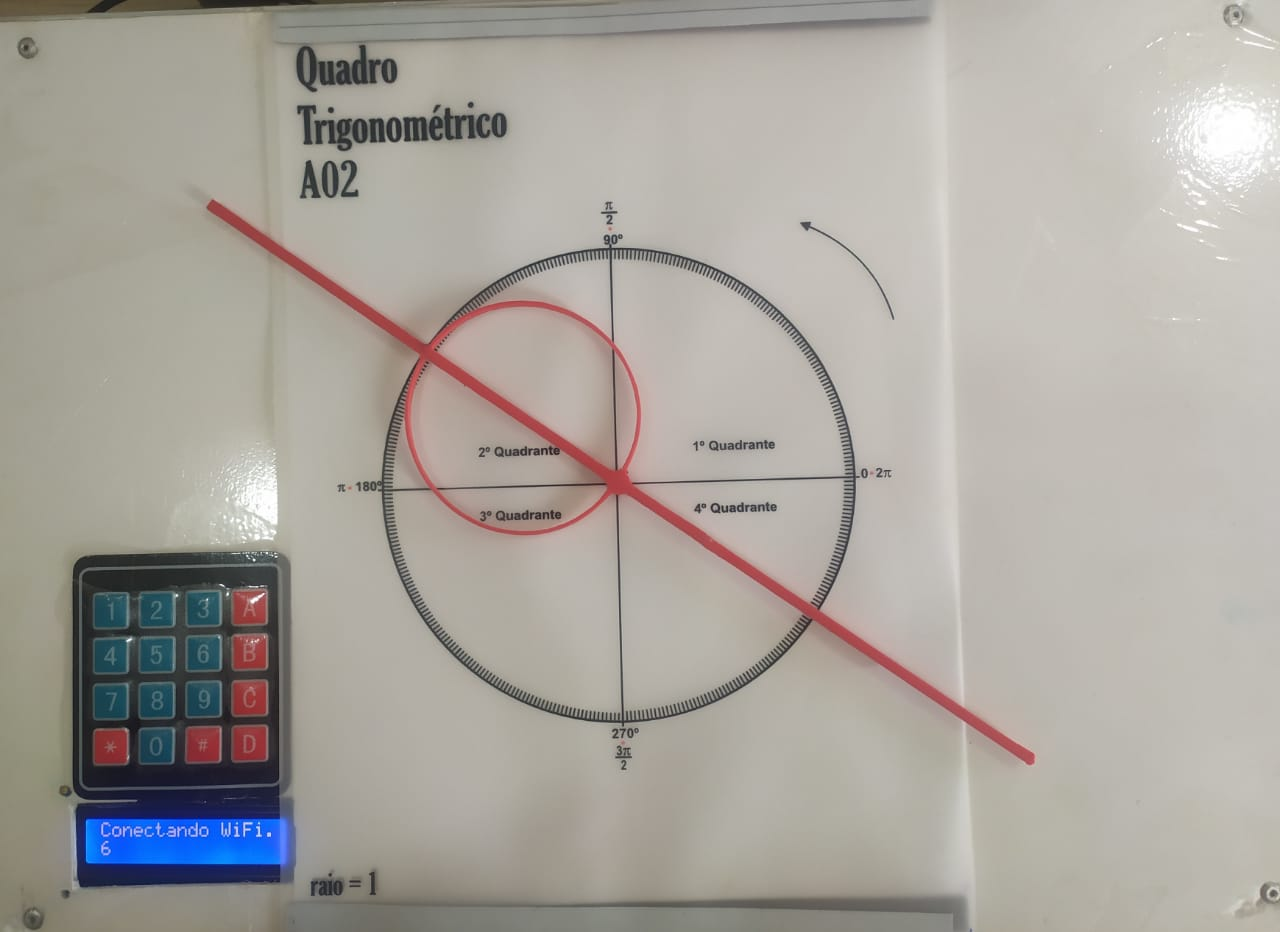
\includegraphics[width=0.7\linewidth]{chapters/proposedMethod/tools/OFVA_quadrotrigonometrico.jpeg}
	\caption{Player Tangível - Interface Física}
	\label{fig:ofva_quadrotrigonometrico}
\end{figure}

Assim, nesta seção de ferramentas, apresentaremos apenas uma das instâncias de OTA implementadas, a fim de facilitar a compreensão do método proposto e do processo de construção de um OTA qualquer, de modo que os demais OTAs serão devidamente apresentados e abordados na seção sobre o estudo de caso (Seção~\ref{sec:estudo_caso1}) e estão disponíveis nos Apêndices~\ref{Chap:AppendixB}, ~\ref{Chap:AppendixC}, ~\ref{Chap:AppendixSeno}, ~\ref{Chap:AppendixCosseno} e~\ref{Chap:AppendixTangente}.

\begin{figure}[htb]
	\centering
	\includegraphics[width=0.7\linewidth]{chapters/proposedMethod/tools/OFVA_VIRTUAL.png}
	\caption{Player Tangível - Interface Virtual}
	\label{fig:ofva_virtual}
\end{figure}

Dessa forma, a Tabela~\ref{tabela:OFV_estudo_caso1} apresenta uma instanciação de um OTA chamado ``Prancha  Trigonométrica - Quadrantes'' no que diz respeito aos aspectos educacionais (nome, descrição geral, descrição educacional, tópicos, modo), dispositivos e gateway. %recursos (físicos e digitais) e serviços. 

A partir desta descrição, pode-se notar que tal objeto tangível tem o objetivo de colaborar com a aprendizagem de estudantes do Ensino Médio, no que diz respeito aos tópicos Trigonometria, Ângulos, Graus e Radianos no processo de identificação dos quadrantes do círculo trigonométrico. %e Razões Trigonométricas (seno, cosseno e tangente).
Para facilitar a descrição do objeto proposto, os dados restantes desta instanciação (entrada, saídas e regras de casos de teste) serão devidamente apresentados na Subseção~\ref{subsubsec:casosdetesteOFVA}.

% \begin{figure}[ht]
% \centering
% \subfigure[ref1][Interface Física]{	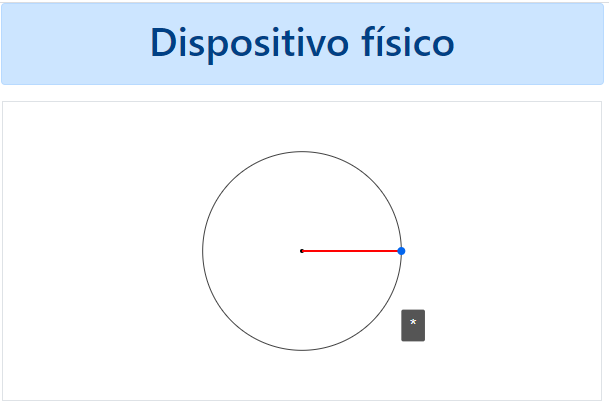
\includegraphics[width=0.3\linewidth]{imgs/OFVA_FISICO.png}}
% \qquad
% \subfigure[ref2][Interface Virtual]{	\includegraphics[width=0.6\linewidth]{imgs/OFVA_VIRTUAL.png}}
% \caption{Estudo de Caso - Player Físico-Virtual}
% \end{figure}

%\begin{figure}[ht]
%	\centering
%    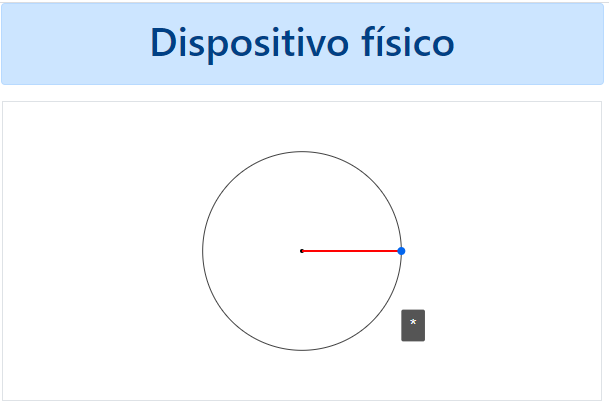
\includegraphics[width=0.7\linewidth]{imgs/OFVA_FISICO.png}
%	\caption{Player Físico-Virtual- Interface Física}
%	\label{fig:ofva_fisico}
%\end{figure}

Em termos de funcionamento, na sua parte física (Figura~\ref{fig:ofva_quadrotrigonometrico}), o objeto proposto coleta os dados referentes à manipulação que o estudante faz de um ponteiro no círculo trigonométrico e os envia para a sua contraparte digital (Figura~\ref{fig:ofva_virtual}). De modo que, toda vez que o estudante altera o ângulo na entidade física, o ângulo também é alterado na entidade digital.

A coleta de dados na entidade física acontece através do uso de sensores de efeito Hall posicionados em cada ângulo a ser detectado e de um ponteiro equipado com ímãs de neodímio, de modo que sempre que o ponteiro ``imantado'' é posicionado sobre um ângulo, o sensor de efeito Hall muda de estado e a entidade digital é atualizada com o valor correspondente.

\begin{figure}[htb]
	\centering
	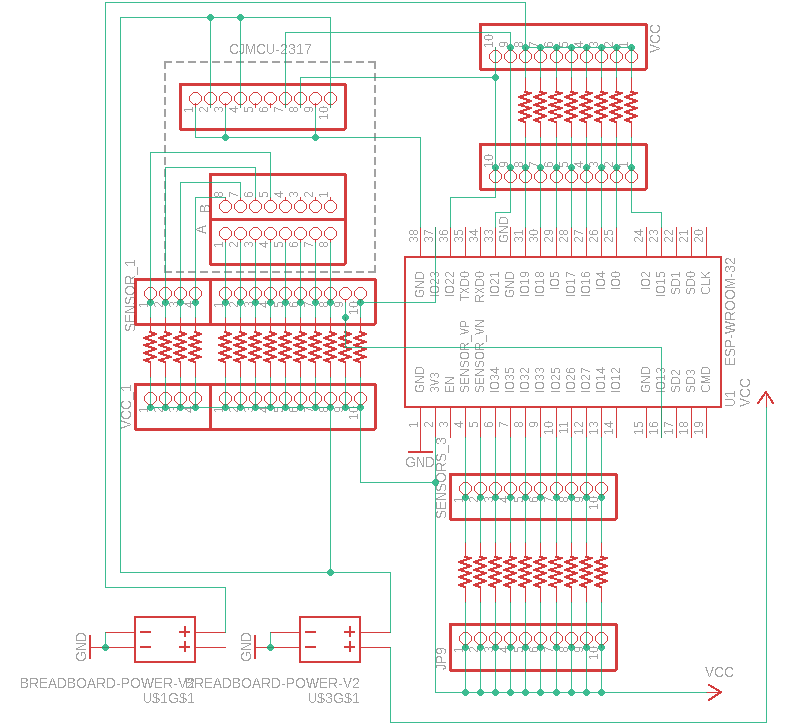
\includegraphics[width=0.9\linewidth]{chapters/proposedMethod/tools/OFVA_FISICO_SENSORES.png}
	\caption{Esquemático do Circuito Elétrico utilizado no Player Tangível}
	\label{fig:ofva_fisico_sensores}
\end{figure}

A Figura~\ref{fig:ofva_fisico_sensores} apresenta o esquemático do circuito elétrico projetado para a instrumentação do manipulativo físico de modo que podemos notar que foi utilizado um microcontrolador ESP-WROOM-32 e um expansor CJMCU-2317 (que usa o chip MCP-23017) para a conexão dos 32 sensores de efeito hall necessários a detecção dos ângulos do círculo trigonométrico. Além disso, como pode ser observado na Figura~\ref{fig:ofva_quadrotrigonometrico}, foram adicionados um Display LCD e um Teclado de Membrana Matricial para melhorar a interação do estudante com o manipulativo, além de proporcionar o fluxo de pareamento necessário entre as duas partes do objeto.

Como proposto na Seção~\ref{section:player}, a comunicação entre as entidades física e virtual do objeto tangível acontece através do uso do protocolo \textit{Websocket}. Assim, foi utilizado o ESP-WROOM-32 de modo que o servidor \textit{Websocket} foi implementado nesta parte do OTA para atuar como um gateway entre as duas entidades e facilitar a atualização dos componentes web da parte virtual do player, uma vez que a entidade digital atua principalmente como um consumidor dos dados provenientes da entidade física e, no caso deste objeto em específico, do valor do ângulo identificado por cada sensor de efeito Hall.

% Ao criar o objeto de aprendizagem, o professor elege cinco possíveis respostas para os alunos marcarem na tela, de modo que a cada alternativa há um peso associado de acordo com o nível de proximidade da resposta correta (que possui o maior peso). Ao final, a plataforma calcula as pontuações dos alunos conforme as métricas apresentadas na Seção~\ref{section:analytics} e os dados informados pelo professor.


% Para melhor entendimento, a Figura~\ref{fig:virtual_casamento} ilustra quatro momentos do estudo de caso. O primeiro momento é quando a criança ouve a situação-problema ao reproduzir um áudio. No segundo momento, a criança inseriu as bolinhas nos dois tubos conforme solicitado e, então, no terceiro momento, ela contou as bolinhas que caídas na peça de baixo. Por fim, a criança seleciona uma das respostas, que pode estar correta ou errada.

% Para o exemplo em questão, considerando a primeira situação-problema da Tabela~\ref{tabela:OFV_estudo_caso1}, caso o estudante selecione a resposta 7 (peso 2) e, em seguida, na segunda situação-problema escolha a alternativa cuja resposta é igual a 4 (peso 4), então, enquanto a nota tradicional é igual a 5,0, a nota ponderada será igual a 7,5.

% \begin{figure}[ht]
% 	\centering
% 	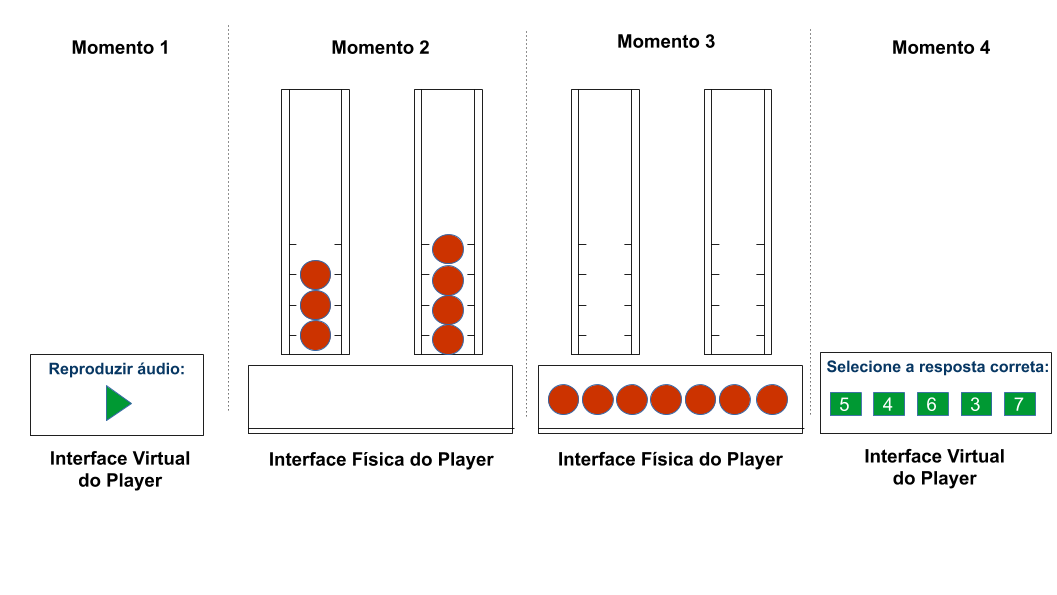
\includegraphics[width=0.9\linewidth]{imgs/Tubo_novo.png}
% 	\caption{Estudo de Caso - Interfaces Virtual e Física}
% 	\label{fig:virtual_casamento}
% \end{figure}

% Vale ressaltar que o objeto de aprendizagem deste estudo de caso pode facilmente ser transformado em outro, por exemplo, em uma máquina de subtração ou de multiplicação.

\subsubsection{Instanciação das Entradas, Saídas e Casos de Teste de um OTA}\label{subsubsec:casosdetesteOFVA}

Para que um objeto tangível de aprendizagem cumpra seu propósito, é importante que haja uma forma de comunicação entre as entidades física e virtual. Desse modo, é necessário especificar as características dos dados a ser enviados e recebidos (entradas e saídas), bem como o que será feito com eles (casos de teste).

\begin{table}[htb!]
	\caption{Recursos: Prancha Trigonométrica - Quadrantes}
	\centering
	\begin{tabular}{|c|c|c|c|c|c|}
		\hline
		\multicolumn{6}{|c|}{\cellcolor[HTML]{C0C0C0}\textbf{RECURSOS}} \\ \hline
		%		\textbf{ID} & 001 \\ \hline
		\multicolumn{6}{|c|}{\cellcolor[HTML]{DEDEDE}\textbf{ENTRADAS FÍSICAS}} \\ \hline
		\textbf{ID} & \textbf{FONTE} & \textbf{RÓTULO} & \textbf{TIPO DE DADO} & \textbf{BLOCOS} & \textbf{JavaScript} \\ \hline
		1 & Físico & EF1 & inteiro & \multicolumn{1}{|l|}{\begin{tabular}[c]{@{}l@{}} \\ 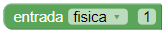
\includegraphics[width=0.2\linewidth]{chapters/appendixC/entrada1.png}  \end{tabular} } & var EF1; \\ \hline
		\multicolumn{6}{|c|}{\cellcolor[HTML]{DEDEDE}\textbf{ENTRADAS DIGITAIS}} \\ \hline
		\textbf{ID} & \textbf{FONTE} & \textbf{RÓTULO} & \textbf{TIPO DE DADO} & \textbf{BLOCOS} & \textbf{JavaScript} \\ \hline
		2 & Virtual & EV1 & inteiro & \multicolumn{1}{|l|}{\begin{tabular}[c]{@{}l@{}} \\ 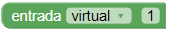
\includegraphics[width=0.2\linewidth]{chapters/appendixC/entrada2.png}  \end{tabular} } & var EV1; \\ \hline
		3 & Virtual & EV2 & ponto flutuante & \multicolumn{1}{|l|}{\begin{tabular}[c]{@{}l@{}} \\ 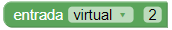
\includegraphics[width=0.2\linewidth]{chapters/appendixC/entrada3.png}  \end{tabular} } & var EV2; \\ \hline
		
		\multicolumn{6}{|c|}{\cellcolor[HTML]{DEDEDE}\textbf{SAÍDAS DIGITAIS}} \\ \hline
		\textbf{ID} & \textbf{FONTE} & \textbf{RÓTULO} & \textbf{TIPO DE DADO} &  \multicolumn{2}{|c|}{\textbf{CONTEÚDO}} \\ \hline
		1 & Virtual & SV1 & String & \multicolumn{2}{|l|}{Mova o ponteiro no sentido horário} \\ \hline
		2 & Virtual & SV2 & String & \multicolumn{2}{|l|}{Mova o ponteiro no sentido anti-horário} \\ \hline
		3 & Virtual & SV3 & String & \multicolumn{2}{|l|}{Posição está correta!} \\ \hline
		4 & Virtual & SV4 & String & \multicolumn{2}{|l|}{\begin{tabular}[c]{@{}l@{}} Ao menos um dos valores informados \\deveria ser menor \end{tabular}} \\ \hline
		5 & Virtual & SV5 & String & \multicolumn{2}{|l|}{\begin{tabular}[c]{@{}l@{}} Ao menos um dos valores informados \\deveria ser maior \end{tabular}} \\ \hline
		6 & Virtual & SV6 & String & \multicolumn{2}{|l|}{Todos os valores estão corretos!} \\ \hline	
		\multicolumn{6}{|c|}{\textbf{BLOCOS}} \\ \hline
		\multicolumn{6}{|c|}{\begin{tabular}[c]{@{}l@{}} \\ 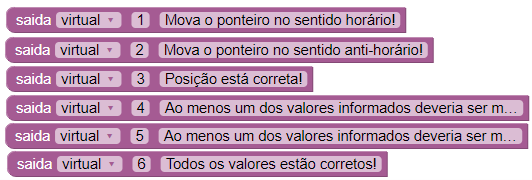
\includegraphics[width=0.8\linewidth]{chapters/appendixC/saidas.png}  \end{tabular}} \\ \hline
		\multicolumn{6}{|c|}{\textbf{JavaScript gerado}} \\ \hline
		\multicolumn{6}{|l|}{\begin{tabular}[c]{@{}l@{}} var SV1 = "Mova o ponteiro no sentido horário!";\\ 			var SV2 = "Mova o ponteiro no sentido anti-horário!";\\ 			var SV3 = "Posição está correta!";\\ 			var SV4 = "Ao menos um dos valores informados deveria ser menor";\\			var SV5 = "Ao menos um dos valores informados deveria ser maior";\\			var SV6 = "Todos os valores estão corretos!"; \end{tabular}} \\ \hline
	\end{tabular}
	\label{tabela:OTA_recursos}
\end{table}	

A Tabela~\ref{tabela:OTA_recursos} apresenta um extrato do Apêndice~\ref{Chap:AppendixB} relativo às entradas e saídas físicas e virtuais de um objeto tangível. Na coluna `Blocos', pode-se observar os blocos criados usando a ferramenta Blockly modificada, enquanto na coluna `JavaScript' tem-se a visão do código gerado automaticamente pela mesma ferramenta, de modo que esta tradução possa ser utilizada pelos outros componentes do objeto.

Como a interface digital do Player Tangível é baseada em tecnologia web, a linguagem JavaScript foi utilizada para definir e tratar os dados recebidos de ambas as entidades física e digital do Player. Assim, a definição das entradas e saídas corresponde a declarações e atribuições dos valores de variáveis JavaScript e a definição das regras dos casos de teste corresponde a criação de uma função nesta mesma linguagem. Além disso, no caso das variáveis de entrada/saída, é necessário indicar se são físicas ou virtuais. Para tanto, como dito anteriormente, foi modificada uma ferramenta baseada em programação em blocos, de modo que a definição de todos esses elementos seja facilitada. %Assim, a Figura~\ref{fig:ofva_entradas} apresenta uma visão da ferramenta implementada, onde 

%\begin{figure}[htb]
%	\centering
%	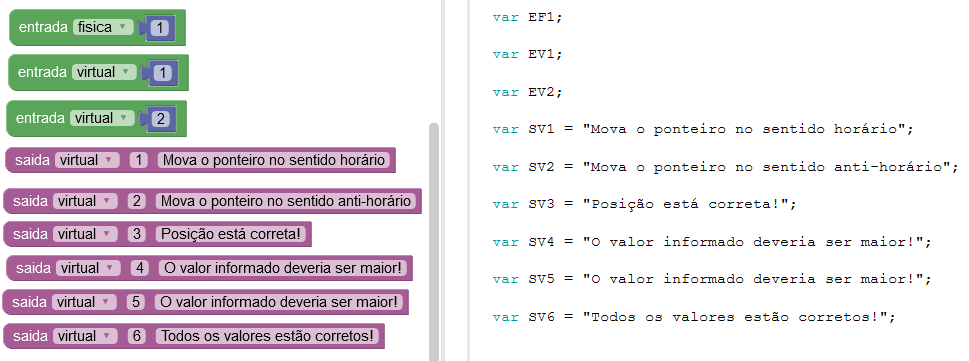
\includegraphics[width=1\linewidth]{imgs/ofva_entradas_saidas.png}
%	\caption{Conjuntos de Entradas e Saídas do OFVA}
%	\label{fig:ofva_entradas}
%\end{figure}

\begin{table}[htb]
	\caption{Definição de um caso de teste}
	\centering
	\begin{tabular}{|l|l|}
		\hline
		\textbf{Item} & \textbf{Descrição} \\ \hline
		\textbf{Rótulo} & \textbf{Início} \\ \hline
		\textbf{Enunciado} & \begin{tabular}[c]{@{}l@{}}Indique o início do primeiro quadrante e informe seu valor em grau e radiano.\end{tabular} \\ \hline
	\end{tabular}
	\label{tabela:OFV_casoteste1}
\end{table}

A definição do caso de teste consiste em estabelecer uma situação-problema a ser resolvida pelo estudante e, de acordo com a necessidade, as regras de \textit{feedback}.%, tal definição consistirá em uma descrição tal como um enunciado. 
Assim, o autor do objeto tangível pode definir tanto o texto do enunciado do caso de teste quanto o seu rótulo (Tabela~\ref{tabela:OFV_casoteste1}). Além disso, quando o objeto tangível prevê o modo ``estudo'' será necessário também indicar o \textit{feedback} a ser dado para uma determinada entrada, visto que o OTA deverá ajudar o estudante a atingir objetivo de aprendizagem através de informações que o levem a melhorar/corrigir suas respostas, de modo que o conhecimento seja construído pelo estudante durante o processo de interação com o material didático.

\begin{table}[htb]
	\caption{Caso de Teste 1 - Regra 1}
	\centering
	\begin{tabular}{|c|c|}
		\hline
		\multicolumn{2}{|c|}{\cellcolor[HTML]{DEDEDE}\textbf{REGRA 1}} \\ \hline
		\textbf{Blocos} & \multicolumn{1}{c|}{\textbf{JavaScript gerado}} \\ \hline
		\multicolumn{1}{|l|}{\begin{tabular}[c]{@{}l@{}} \\ 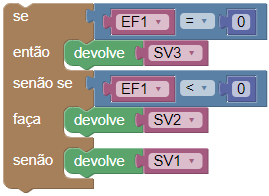
\includegraphics[width=0.4\linewidth]{chapters/appendixB/c1r1.png}  \end{tabular}
		} & \begin{tabular}[c]{@{}l@{}} if((EF1 == 0))\{   return SV3; \}\\ else if ((EF1 < 0))\{   return SV2; \}\\ else \{   return SV1; \} \end{tabular} \\ \hline
	\end{tabular}
	\label{tabela:OTA_c1r1}
\end{table}
 
Essa abordagem foi escolhida para que diversas estratégias pedagógicas pudessem ser utilizadas, uma vez que o modo ``estudo'' permite que o estudante sinta que está construindo conhecimento através da construção ou descoberta dos elementos que compõem o objeto tangível, ao invés de sentir que está sendo simplesmente avaliado.

%\begin{figure}[ht]
%	\centering
%	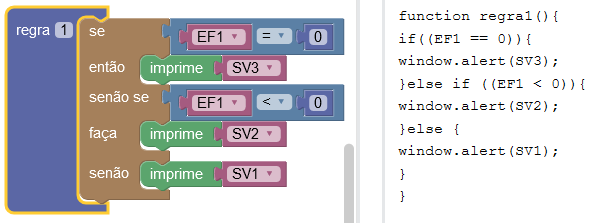
\includegraphics[width=0.8\linewidth]{imgs/ofva_regra1.png}
%	\caption{Regra 1 - Caso de Teste Q1-Início}
%	\label{fig:ofva_regra1}
%\end{figure}

\begin{table}[htb]
	\caption{Caso de Teste 1 - Regra 2}
	\centering
	\begin{tabular}{|c|c|}
		\hline
		\multicolumn{2}{|c|}{\cellcolor[HTML]{DEDEDE}\textbf{REGRA 2}} \\ \hline
		\textbf{Blocos} & \multicolumn{1}{c|}{\textbf{JavaScript gerado}} \\ \hline
		\multicolumn{1}{|l|}{\begin{tabular}[c]{@{}l@{}} \\ 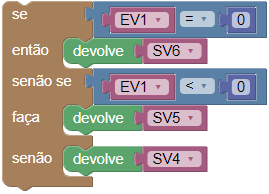
\includegraphics[width=0.4\linewidth]{chapters/appendixB/c1r2.png}  \end{tabular}
		} &  \begin{tabular}[c]{@{}l@{}}if((EV1 == 0))\{   return SV6; \}\\ else if ((EV1 < 0))\{   return SV5; \}\\ else \{   return SV4; \} \end{tabular}  \\ \hline
	\end{tabular}
	\label{tabela:OTA_c1r2}
\end{table}

Através de programação em blocos, são definidas regras para avaliação das entradas fornecidas pelo estudante, de modo que um código em JavaScript seja gerado automaticamente para ser incorporado a interface digital do Player. As Tabelas~\ref{tabela:OTA_c1r1}, \ref{tabela:OTA_c1r2} e \ref{tabela:OTA_c1r3} apresentam as definições das regras para o caso de teste apresentado na Tabela~\ref{tabela:OFV_casoteste1}, onde a atividade em questão prevê que o estudante deve encontrar os valores dos ângulos de início do primeiro quadrante, respectivamente, 0° e 0 rad.
 %As Figuras~\ref{fig:ofva_regra1}, \ref{fig:ofva_regra2} e \ref{fig:ofva_regra3} apresentam as definições das regras para o caso de teste da Tabela~\ref{tabela:OFV_casoteste1}


%\begin{figure}[ht]
%	\centering
%	\includegraphics[width=0.8\linewidth]{imgs/ofva_regra2.png}
%	\caption{Regra 2 - Caso de Teste Q1-Início}
%	\label{fig:ofva_regra2}
%\end{figure}

%\begin{figure}[ht]
%	\centering
%	\includegraphics[width=0.8\linewidth]{imgs/ofva_regra3.png}
%	\caption{Regra 3 - Caso de Teste Q1-Início}
%	\label{fig:ofva_regra3}
%\end{figure}


\begin{table}[htb]
	\caption{Caso de Teste 1 - Regra 3}
	\centering
	\begin{tabular}{|c|c|}
		\hline
		\multicolumn{2}{|c|}{\cellcolor[HTML]{DEDEDE}\textbf{REGRA 3}} \\ \hline
		\textbf{Blocos} & \multicolumn{1}{c|}{\textbf{JavaScript gerado}} \\ \hline
		\multicolumn{1}{|l|}{\begin{tabular}[c]{@{}l@{}} \\ \includegraphics[width=0.4\linewidth]{chapters/appendixB/c1r3.png}  \end{tabular}
		} & \begin{tabular}[c]{@{}l@{}}if((EV2 == 0))\{   return SV6; \}\\ else if ((EV2 < 0))\{   return SV5; \}\\ else \{   return SV4; \} \end{tabular}  \\ \hline
	\end{tabular}
	\label{tabela:OTA_c1r3}
\end{table}

Além disso, pode-se observar que as regras definem o \textit{feedback} dado de acordo com a entrada fornecida pelo estudante, de modo que esta etapa corresponde ao processo de associação entre as entradas e saídas físicas e digitais, tal como previsto na Figura~\ref{fig:bpmn_ofva_casos}, que apresenta o subprocesso de definição de serviços. Por fim, o restante da definição desta atividade pode ser encontrado no Apêndice~\ref{Chap:AppendixB}.

Para que haja o acompanhamento da aprendizagem é necessário definir também os parâmetros das métricas de avaliação conforme os modelos de processos apresentados na Subseção~\ref{subsec:aplicacao_metricasOFVA}. Tal ação somente pode ser executada após a criação do OTA no Compositor e através do módulo Analíticos.

\subsection{Servidor}

O Servidor é o módulo responsável pela criação e gerenciamento da sala de aula virtual, permitindo o acesso dos estudantes ao material didático e a consolidação dos dados coletados pelo Player. 

É importante ressaltar que, neste trabalho, o servidor foi implementado em dois serviços distintos, uma vez que a implementação relacionada aos objetos de aprendizagem tradicionais está em estágio avançado e sendo executada em servidores na nuvem, tendo sido implementada usando o \textit{Framework} Angular e \textit{NodeJS}.

A parte do servidor que provê o objeto tangível foi implementada em duas partes, sendo a primeira parte uma API (do inglês, Interface de Programação de Aplicação) desenvolvida utilizando a linguagem de programação \textit{Python} e o \textit{Framework Django}, de modo que esta API concentra todas as regras de negócio (casos de teste, regras de validação, acesso e administração). 

A segunda parte corresponde ao \textit{frontend} - isto é, a interface gráfica da entidade virtual com a qual o estudante interage diretamente - foi desenvolvida em \textit{Typescript} através do \textit{Framework} Angular de modo que fossem providos tanto a interação do estudante com a entidade digital, quanto a conexão via \textit{websocket} com a entidade física.

Os dados coletados por ambos os serviços são armazenados em um banco de dados \textit{MongoDB} que é do tipo não relacional (\textit{NoSQL}) de modo que os \textit{logs} das atividades dos estudantes em ambas as interfaces (virtual ou tangível) possam ser recuperados e utilizados para o cálculo das diversas métricas de aprendizagem propostas neste trabalho. 

\begin{figure}[htb]
	\centering
	\includegraphics[width=0.8\linewidth]{chapters/proposedMethod/tools/servidor_log.png}
	\caption{Exemplo de Log de um objeto de aprendizagem tradicional}
	\label{fig:servidor_log}
\end{figure}

Assim, a Figura~\ref{fig:servidor_log} apresenta um dado relativo a resposta dada por um estudante a uma questão de múltipla-escolha cujo identificador é `592', a resposta fornecida corresponde a alternativa `C'. É possível observar que o log armazena também informação relacionada ao momento em que o dado foi capturado (\textit{timestamp}), o que possibilita o cálculo das métricas baseadas em tempo.

\begin{figure}[htb!]
	\centering
	\includegraphics[width=0.4\linewidth]{chapters/proposedMethod/tools/servidor_log_tangivel.png}
	\caption{Exemplo de Log de um OTA}
	\label{fig:log_tangivel}
\end{figure}

A Figura~\ref{fig:log_tangivel} apresenta uma instância do log de um objeto tangível armazenado no banco de dados, onde é possível notar que o dado corresponde a entrada física de rótulo `ef1' cujo valor é relativo ao ângulo '100'.

% % Para criar a sala de aula virtual, gerenciar as modificações nos players dos estudantes a partir dos níveis de ajuda sob demanda e criar os \textit{logs}, o Servidor utiliza um conjunto de \textit{scripts} em Python implementados a partir do microframework Flask.

% % Vale ressaltar que, além de ser um exemplo de tela do Player exibindo um Questionário, a Figura~\ref{fig:player_adaptacao} também exibe as modificações dos três níveis de ajuda já ativadas pelo Servidor para a `Questão 1 - Principal' no Player de um aluno.

% % \begin{figure}[ht]
% % 	\centering
% % 	\includegraphics[width=1\linewidth]{imgs/tools/servidor_log}
% % 	\caption{Servidor - Log do Aluno 01}
% % 	\label{fig:servidor_log}
% % \end{figure}

% % A Figura~\ref{fig:servidor_log} introduz o log do `Aluno 01', onde é possível verificar o \textit{timestamp}, a página destino (i.e: questionario.html) e a informação ou ajuda exibidas para o aluno. Onde, `Q:1' e `Q:2' (linhas 1 e 12) indicam que o aluno abriu as Questões 01 e 02, respectivamente e, as letras `D' e `C' indicam que ele utilizou ajuda sob demanda. Nesse caso, foram utilizados dois níveis: (D) Sugestão e (C) Conteúdo. O nível de ajuda relativo a troca de Questão Principal para Questão Alternativa está relacionado a identificação `H:', que indica que a questão, a dica ou o conteúdo visualizados tem ligação com a Questão Principal. Assim, caso estivem ligados a uma Questão Alternativa, a identificação seria `E:'.


\subsection{Analíticos}

% % O módulo responsável pelas métricas foi implementado utilizando um conjunto de Shell Scripts. Tais scripts extraem informações dos logs gerados pelo servidor e realizam a análise de acordo com as métricas apresentadas na Seção~\ref{section:analytics}. Além dos cálculos e geração das métricas, estes \textit{scripts} também plotam os gráficos a serem exibidos para o professor.

O módulo responsável pelas métricas foi implementado utilizando um conjunto de scripts em linguagem \textit{Python}. Tais scripts extraem informações dos logs armazenados no banco de dados pelo servidor e realizam os cálculos das métricas apresentadas na Seção~\ref{section:analytics}. O resultados destes cálculos são guardados em um novo banco de dados não relacional, de modo que possam ser utilizados para acompanhamento e avaliação da aprendizagem dos estudantes e das turmas que utilizaram o ambiente proposto.  %Além dos cálculos e geração das métricas, estes \textit{scripts} também plotam os gráficos a serem exibidos para o professor.

%\begin{figure}[htb]
%	\centering
%	\includegraphics[width=0.6\linewidth]{chapters/proposedMethod/tools/analiticos_ponderada_entradas.png}
%	\caption{Exemplo - Média Ponderada}
%	\label{fig:media_ponderada_entradas_exemplo}
%\end{figure}

\begin{figure}[htb]
	\centering
	\subfigure[ref1][Por Entrada]{\includegraphics[width=6.8cm]{chapters/proposedMethod/tools/analiticos_ponderada_entradas_.png}\label{fig:media_ponderada_entradas_exemplo}}
	\qquad
	\subfigure[ref2][Por Caso de Teste]{\includegraphics[width=7.3cm]{chapters/proposedMethod/tools/analiticos_ponderada_casos.png}\label{fig:media_ponderada_casos_exemplo}}
	\caption{Exemplo de instâncias da Média Ponderada}
	\label{fig:media_ponderada_exemplo}
\end{figure}

A Figura~\ref{fig:media_ponderada_entradas_exemplo} ilustra três instâncias do banco de dados que armazenam o valor da média ponderada de um estudante relativo às entradas `EF1', `EV1' e `EV2', respectivamente. No exemplo em questão, a média ponderada foi calculada considerando que as entradas e os casos de teste são agrupados de uma vez, para ilustrar a liberdade de escolha que o professor tem com relação ao acompanhamento e avaliação do estudante, conforme proposto no modelo de processos da Figura~\ref{fig:bpmn_metricas}. 

%\begin{figure}[htb]
%	\centering
%	\includegraphics[width=0.5\linewidth]{chapters/proposedMethod/tools/analiticos_ponderada_casos.png}
%	\caption{Exemplo - Média Ponderada}
%	\label{fig:media_ponderada_casos_exemplo}
%\end{figure}

Além disso, como é possível definir se o cálculo das métricas vai levar em consideração os casos de teste ou as entradas, é preciso entender que essa decisão influencia no modo como a métrica é calculada já que, para o cálculo do ponto de vista do caso de teste, todas as entradas serão agrupadas por caso de teste, de modo que a avaliação das resposta do estudante será feita com esse parâmetro de base. Assim, a Figura~\ref{fig:media_ponderada_casos_exemplo} ilustra as notas de um estudante calculadas de acordo com essa possibilidade, onde cada instância corresponde a um caso de teste diferente (rótulo `fonte').

\begin{figure}[htb]
	\centering
	\includegraphics[width=0.5\linewidth]{chapters/proposedMethod/tools/NCQ_topicos.png}
	\caption{Parâmetros do NCQ - Tópicos}
	\label{fig:NCQ_topicos}
\end{figure}

No caso de escolher o método das entradas, então, será levado em consideração o tópico específico de cada entrada, por exemplo, na Figura~\ref{fig:NCQ_entradas} pode-se observar que cada entrada de cada caso de teste corresponde a um tópico (ie: `Radianos', `Leitura de instrumento',...), de modo que cada tópico possui seu próprio nível de dificuldade (Figura~\ref{fig:NCQ_topicos}).

\begin{figure}[htb]
	\centering
	\includegraphics[width=1\linewidth]{chapters/proposedMethod/tools/NCQ_entradas.png}
	\caption{Parâmetros do NCQ - Entradas}
	\label{fig:NCQ_entradas}
\end{figure}

É importante ressaltar que todos dados relativos aos objetos de aprendizagem, seja os objetos tradicionais, seja os objetos tangíveis, estão armazenados em bancos de dados do tipo relacional (SQL), de modo que os diversos serviços possam facilmente fazer consultas e inserções a partir de uma hierarquia que leva em consideração os autores dos objetos de aprendizagem e, tanto quanto possível, o preenchimento automático do metadados a partir do perfil apresentado no Apêndice~\ref{Chap:AppendixA}, que já foi comentado previamente.

\begin{table}[htb!]
	\caption{Nota Ponderada - Caso de Teste 1 - EF1}
	\centering
	\begin{tabular}{|c|c|}
		\hline
		\multicolumn{2}{|c|}{\cellcolor[HTML]{DEDEDE}\textbf{NP - CASO 1 - EF1}} \\ \hline
		\textbf{Blocos} & \multicolumn{1}{c|}{\textbf{Python gerado}} \\ \hline
		\multicolumn{1}{|l|}{\begin{tabular}[c]{@{}l@{}} \\ \includegraphics[width=0.6\linewidth]{chapters/appendixAnalytics/CASO1NPEF1.png}  \end{tabular}
		} & \begin{tabular}[c]{@{}l@{}}import math \\ \# Nota Ponderada - Caso 1\\ def EF1CASO1(EF1):\\ \quad global RE, PESO\\ \quad RE = 0\\ \quad	if math.fabs(RE - EF1) == 0:\\	\quad \quad PESO = 4\\ \quad elif math.fabs(RE - EF1) <= 10:\\ \quad \quad PESO = 3\\	\quad elif math.fabs(RE - EF1) <= 20:\\ \quad \quad	PESO = 2\\ \quad elif math.fabs(RE - EF1) <= 30:\\ \quad \quad PESO = 1\\ \quad	else:\\ \quad \quad	PESO = 0\\ return PESO
	 \end{tabular}  \\ \hline
	\end{tabular}
	\label{tabela:OTA_C1EF1}
\end{table}

Por fim, a Tabela~\ref{tabela:OTA_C1EF1} apresenta uma instância da definição de parâmetros para o cálculo da Nota Ponderada do Caso de Teste previamente instanciado na Seção~\ref{subsubsec:casosdetesteOFVA}, onde pode-se observar que é gerado um código-fonte na linguagem Python a partir do blocos definidos em Analíticos. As instâncias restantes desta atividade podem ser encontradas no Apêndice~\ref{Chap:AppendixAnaliticos}. Os parâmetros das métricas para os Exercícios 2, 3, 4 e 5, encontram-se nos Apêndices~\ref{Chap:AppendixAnaliticosA02}, \ref{Chap:AppendixAnaliticosA03}, \ref{Chap:AppendixAnaliticosA04} e \ref{Chap:AppendixAnaliticosA05}, respectivamente.

% % -----------------------------------------------------------------
% % => Summary - PROPOSED METHOD 
% % -----------------------------------------------------------------
\section{Resumo}
\label{summary:ProposedMethod}

Neste capítulo descrevemos uma abordagem para inserção de tecnologia em sala de aula, proposta a partir de uma arquitetura com quatro componentes principais, possibilitando o uso de objetos tangíveis de aprendizagem em sala de aula de modo a permitir o acompanhamento/avaliação da aprendizagem e a fornecer mais elementos e análises a partir de dados de interação dos estudantes com os diversos recursos educacionais disponíveis.
% a avaliação de conteúdo baseada em questões com ajuda sob demanda, além de permitir a verificação de outros elementos que ajudem o professor a entender melhor o desenvolvimento dos estudantes.

Na Seção~\ref{section:composer}, foi detalhado o modelo do Compositor, primeiro elemento da abordagem proposta, que é o responsável pelo processo de autoria dos objetos de aprendizagem inseridos e a montagem da aula em si de modo que tais objetos possam ser associados por um professor como parte de uma mesma aula. Ainda nessa seção, foram apresentados (i) novos elementos relacionados ao objeto de aprendizagem questionário, que servirão de parâmetro para algumas das métricas propostas; e (ii) uma proposta de modelo para um objeto tangível de aprendizagem de modo que os atributos desse objeto possibilitem sua inserção, uso e funcionamento dentro de um ambiente de aprendizagem. Ademais, também foi proposto utilizar o perfil ``PM-OBAA-FULL'' como padrão de metadados.

Na Seção~\ref{section:service}, foi apresentada a parte do ambiente de aprendizagem responsável pelo gerenciamento da sala de aula virtual e pela consolidação das informações coletadas pelos dispositivos dos alunos durante a aula. Nesta seção, foram introduzidas modificações relacionadas ao funcionamento dos objetos tangíveis de aprendizagem de modo a haver compatibilidade com o modelo de objeto tangível proposto.

A Seção~\ref{section:player} apresentou a comunicação e o funcionamento interno do Player Tangível, que é a interface de interação do estudante com o sistema, mas que, também, é o meio através do qual os dados dessa interação são coletados e enviados para o Servidor. Além disso, foram apresentados os componentes que possibilitam o funcionamento das interface física e digital, além da definição formal do processo de pareamento e comunicação (trocas de mensagens) entre as entidades do objeto tangível.

A Seção~\ref{section:analytics} introduziu novas métricas de aprendizagem com o objetivo de melhorar a verificação e o entendimento da aprendizagem dos estudantes ao longo de uma rotina educativa. Assim, são apresentadas as métricas: Nota Tradicional, Nota Ponderada, Dúvida da Questão, Grau de Assertividade, Tempo de Resposta, Prioridade, Nível de Compreensão da Questão e Nível de Compreensão do Questionário. Por fim, nesta mesma seção, são apresentados diagramas de modelos de processos que formalizam o passo-a-passo para aplicação das métricas propostas a objetos tangíveis.
%Desvio da Resposta, Dúvida da Questão, Grau de Assertividade, Tempo de Resposta, Nível de Desordem, Desvio do Conjunto, Prioridade, Nível de Compreensão da Questão e Nível de Compreensão do questionário.

% Por fim, a Seção~\ref{section:inteligencia} apresenta um novo módulo da arquitetura cujo objetivo é utilizar agentes inteligentes que façam recomendações e notificações baseadas nas análises provenientes do Módulo Analytics.

Finalmente, a Seção~\ref{section:Tools} apresentou alguns detalhes da implementação feita com a finalidade de experimentar e validar o método proposto nas Seções~\ref{section:composer},~\ref{section:service},~\ref{section:player},~\ref{section:analytics} deste capítulo.